% pii — User and Administration Manual
% Template: kaobook · compiled through lnx's texlive container
\documentclass[
	fontsize=10pt,
	twoside=false,
	secnumdepth=2,
	open=any,
]{kaobook}

\usepackage[english]{babel}
\usepackage[style=english]{csquotes}
\usepackage{amsmath, amssymb}
\usepackage{booktabs}
\usepackage{longtable}
\usepackage{array}
\usepackage{listings}
\usepackage{xcolor}
\usepackage{hyperref}
\usepackage{graphicx}
\usepackage{caption}% captions outside floats: kaobook's figure env recurses around tikz

% TikZ: every concept in these manuals is drawn, not only described.
\usepackage{tikz}
\usetikzlibrary{arrows.meta, positioning, calc, shapes.geometric, shapes.misc,
                fit, backgrounds, patterns, decorations.pathreplacing}
\usepackage{pgfplots}
\pgfplotsset{compat=1.18}

% One visual vocabulary for both manuals, so a box means the same thing in every figure.
\tikzset{
  box/.style={draw, rounded corners=2pt, fill=blue!4, align=center,
              inner sep=4pt, font=\footnotesize, minimum height=1.0cm},
  store/.style={draw, cylinder, shape border rotate=90, aspect=0.25, fill=orange!8,
                align=center, inner sep=3pt, font=\footnotesize, minimum height=1.1cm},
  model/.style={draw, rounded corners=8pt, fill=purple!8, align=center,
                inner sep=4pt, font=\footnotesize, minimum height=1.0cm},
  verdict/.style={draw, diamond, aspect=1.6, fill=green!8, align=center,
                  inner sep=1pt, font=\scriptsize},
  port/.style={font=\scriptsize\itshape, inner sep=1pt, fill=white},
  flow/.style={-{Latex[length=2mm]}, thick},
  soft/.style={-{Latex[length=2mm]}, thick, dashed, gray!70},
  back/.style={-{Latex[length=2mm]}, thick, red!60!black, dashed},
  group/.style={draw, dashed, rounded corners=4pt, inner sep=8pt, gray!60},
}


% Code listings: the manual is full of commands and configuration snippets.
\definecolor{codebg}{RGB}{247,247,249}
\lstset{
	basicstyle=\ttfamily\footnotesize,
	backgroundcolor=\color{codebg},
	frame=single,
	framesep=3pt,
	breaklines=true,
	columns=fullflexible,
	keepspaces=true,
	showstringspaces=false,
	postbreak=\mbox{\textcolor{gray}{$\hookrightarrow$}\space},
}

\titlehead{pii \textperiodcentered{} personal information index}
\title{User and Administration Manual}
\author{Marcelo Correa}
\date{Version 0.2.0 \textperiodcentered{} build 2026-11-04 10:27 UTC \textperiodcentered{} commit \texttt{c05f3d1e4dd3}}
\publishers{Setup, daily usage and the technical reference}


% Short names, same meanings: b box · s store · m model · v verdict · p port · f flow ·
% sf soft edge · bk back edge · g group. Both books accept either spelling.
\tikzset{
  b/.style={draw, rounded corners=2pt, fill=blue!4, align=center, inner sep=4pt, font=\footnotesize},
  s/.style={draw, cylinder, shape border rotate=90, aspect=0.25, fill=orange!8, align=center, inner sep=3pt, font=\footnotesize},
  m/.style={draw, rounded corners=8pt, fill=purple!8, align=center, inner sep=4pt, font=\footnotesize},
  v/.style={draw, diamond, aspect=1.6, fill=green!8, align=center, inner sep=1pt, font=\scriptsize},
  p/.style={font=\scriptsize\itshape, inner sep=1pt, fill=white},
  f/.style={-{Latex[length=2mm]}, thick},
  sf/.style={-{Latex[length=2mm]}, thick, dashed, gray!70},
  bk/.style={-{Latex[length=2mm]}, thick, red!60!black, dashed},
  g/.style={draw, dashed, rounded corners=4pt, inner sep=8pt, gray!60},
}

\begin{document}

\frontmatter
\maketitle

\uppertitleback{\titlehead}
\lowertitleback{
	\textbf{About this manual} \\
	This is the operator's book. It covers installation, configuration, the daily
	commands, backup and retention, and a reference for every command and setting.
	It does not explain the internals: that is the other manual,
	\textit{pii --- Architecture and Development Manual}.

	\medskip
	\textbf{Scope} \\
	Written for the person who installs pii on a host and keeps it running, and for
	the user who asks it questions, runs its graphs and reads its reports.

	\medskip
	\textbf{Version} \\
	Everything here was measured against pii 0.2.0. Where a behaviour is newer than
	that release it is marked with the row that introduced it.

	\medskip
	\textbf{Colophon} \\
	Typeset with \LaTeX{} using the \href{https://www.latex-templates.com/template/kaobook}{kaobook}
	template, compiled through the shared texlive container on \texttt{lnx}.
}

\tableofcontents

\mainmatter
\chapter{What pii is}

\label{ch:what}

pii is a \emph{personal information index}: one Rust binary that keeps stores of runs,
memory, entities and lessons on disk, executes \emph{graphs} --- small programs written as
data --- on a daemon, and records every state change in a journal that can be replayed,
counted and audited. This chapter answers three questions before the rest of the manual
asks anything of you: what the program does, what it is made of, and which of its answers
you are allowed to trust. Every number and path in this chapter was read from the
repository at the revision the manual was built from, not from a design document; where a
mechanism exists because something failed, the failure is named.

It is not a chat application that happens to have a database. It is an execution engine
whose every action leaves evidence, and the questions you will ask of it are of the form
\enquote{what ran, what did it decide, and can I prove it}. The design follows from that:
if a fact cannot be shown from the journal or from a store, pii treats it as unknown rather
than as true. The three exit codes of \texttt{pii health} are the smallest example --- a
daemon that answers from a different build than your client is reported as drift, not as
health.

\section{The three things it does}

\begin{enumerate}
	\item \textbf{Runs work.} A graph is a set of nodes --- ask a model, run a command,
	judge a set of exit criteria, call another graph --- connected by named ports. pii
	executes it, journals each transition, and returns a verdict rather than a transcript.
	\item \textbf{Remembers what it learned.} Runs, node-call events, memory documents,
	entities and lessons live in redb stores with counters, snapshots and, since the
	retention row, an age-based policy that bounds them.
	\item \textbf{Tells the truth about itself.} \texttt{pii health} answers from a record
	kept current by the write path rather than by replaying history at read time, and the
	answer names the build, the config file's hash, each store's path and format version,
	and the mounts the sandbox actually granted.
\end{enumerate}

Those three are one mechanism seen from three sides. The journal is what makes a verdict
provable; the stores are what make a second run cheaper than the first; the identity
payload is what makes an upgrade, a rollback or a wrong state directory visible instead of
merely suspected.

\section{The shape of the system}

The workspace is twenty-two \texttt{pii-*} crates plus \texttt{xtask}, the internal
tool that runs the quality gate. Four binaries come out of it: \texttt{pii} (the daemon
and the command line in one file), \texttt{pii-mcp} (a Model Context Protocol server),
\texttt{pii-web} (a small HTTP surface) and \texttt{pii-evolve}. Only \texttt{pii} is
required to operate the product; the installer places the other three beside it, and
\texttt{pii-mcp} is staged as \texttt{pii-mcp.new} rather than swapped in, because its
callers are other programs whose behaviour has to be measured before the swap.

\begin{longtable}{@{}p{0.20\textwidth}p{0.30\textwidth}p{0.42\textwidth}@{}}
	\toprule
	\textbf{Binary} & \textbf{Crate} & \textbf{What it is for} \\
	\midrule
	\endhead
	\texttt{pii} & \texttt{pii-cli} & The command line, and the daemon when invoked as
	\texttt{pii daemon}. Embeds the engine in-process for a one-shot prompt. \\
	\texttt{pii-mcp} & \texttt{pii-mcp} & A Model Context Protocol server over the same
	engine, for tools that speak MCP. Installed as \texttt{.new}; the swap is an operator
	step. \\
	\texttt{pii-web} & \texttt{pii-web} & A separate HTTP binary, not linked into
	\texttt{pii}. \\
	\texttt{pii-evolve} & \texttt{pii-evolve} & A separate evolution binary, not linked
	into \texttt{pii}. \\
	\bottomrule
\end{longtable}

Inside \texttt{pii} the layering is strict, and it is the reason an operator can reason
about failure at all. The control commands --- \texttt{run}, \texttt{queue},
\texttt{health}, \texttt{memory}, \texttt{skill} --- never open a store: they dial
\texttt{control.sock}. The daemon owns the stores, the run pool, the timer wheel and the
channels. The engine executes one run at a time per worker and journals every node
transition. \texttt{pii-store} is the only crate that knows redb exists, and the commands
that do open a file (\texttt{store}, \texttt{backup}, \texttt{restore}, and the offline
\texttt{graph run} and \texttt{graph trace} with \texttt{--db}) take redb's exclusive lock
and refuse while a daemon holds it.

\begin{center}
\resizebox{\linewidth}{!}{
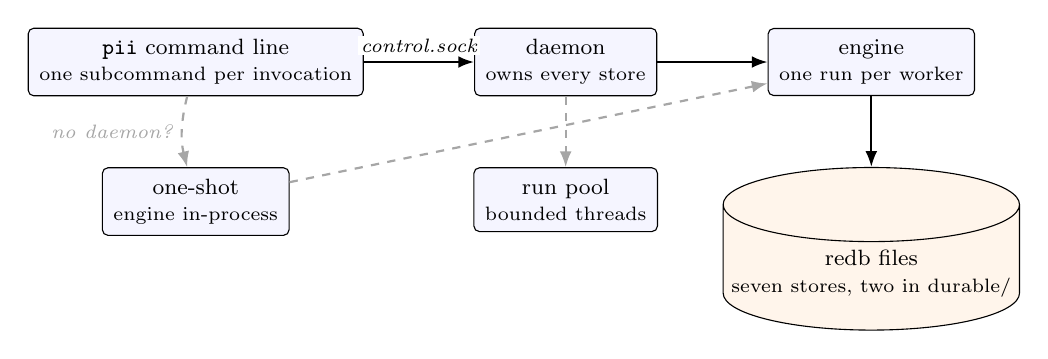
\begin{tikzpicture}[node distance=9mm and 14mm]
  \node[b] (cli) {\texttt{pii} command line\\\scriptsize one subcommand per invocation};
  \node[b, right=of cli] (daemon) {daemon\\\scriptsize owns every store};
  \node[b, right=of daemon] (engine) {engine\\\scriptsize one run per worker};
  \node[s, below=of engine] (redb) {redb files\\\scriptsize seven stores, two in durable/};
  \node[b, below=of daemon] (pool) {run pool\\\scriptsize bounded threads};
  \node[b, below=of cli] (oneshot) {one-shot\\\scriptsize engine in-process};
  \draw[f] (cli) -- node[p,above=2pt,midway]{control.sock} (daemon);
  \draw[f] (daemon) -- (engine);
  \draw[f] (engine) -- (redb);
  \draw[sf] (daemon) -- (pool);
  \draw[sf] (cli) to[bend right=14] node[p,left=2pt,midway]{no daemon?} (oneshot);
  \draw[sf] (oneshot) -- (engine);
\end{tikzpicture}}
\captionof{figure}{Two ways in and one owner. The command line either reaches the daemon over
its socket, or --- for a one-shot prompt only --- builds the engine in its own process. Notice
that the store has exactly one writer, which is what makes an offline command refuse rather than
contend.}
\end{center}

The distinction matters in practice. \texttt{pii store compact} and \texttt{pii backup}
are two of the commands that do open the files, and both refuse while a daemon holds them
instead of copying a store mid-write. Everything else --- \texttt{run}, \texttt{queue},
\texttt{health}, \texttt{memory}, \texttt{skill} --- is a protocol call.

\section{A graph is data}

A graph file is TOML with five top-level facts: a \texttt{name} (the key \texttt{pii run
start} resolves), an \texttt{entry} node, an optional \texttt{exit} node, a \texttt{caps}
list, and an optional \texttt{[limits]} table. Nodes and edges follow. This is the
beginning of the development queue's own graph, at the revision this manual describes:

\begin{lstlisting}[language=bash]
name = "queue"
entry = "select"
exit = "record"
caps = ["spawn", "proc", "fs_read", "fs_write"]

[limits]
max_wall_ms = 6000000

[[node]]
id = "select"
kind = "select"

[[node]]
id = "implement"
kind = "call"
graph = "spec"
sha256 = "771d098b39db7369dd71ed1fb23ffa63b90b25fed7788c830e4bfb214c424443"
caps = ["spawn", "proc", "fs_read", "fs_write"]

[[edge]]
from = "select"
port = "ok"
to = "implement"
kind = "data"
\end{lstlisting}

Three things in those lines carry most of the design. The \texttt{sha256} on a
\texttt{call} is a pin: the callee is spliced into the host at load time, so a change to
the callee invalidates the pin until someone re-pins it deliberately. The \texttt{caps} on
the call node are the host's promise that it holds what the callee needs. And the
\texttt{port} on an edge is a name, not a boolean --- \texttt{select} leaves by
\texttt{ok}, \texttt{empty} or \texttt{blocked}, and each can go somewhere different.

\begin{center}
\resizebox{\linewidth}{!}{
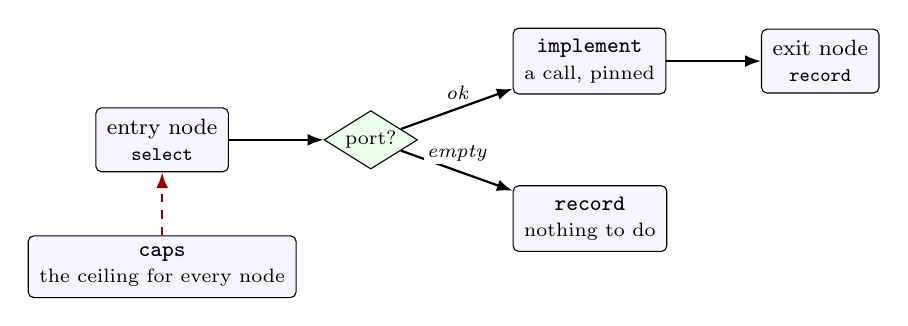
\begin{tikzpicture}[node distance=8mm and 12mm]
  \node[b] (entry) {entry node\\\scriptsize \texttt{select}};
  \node[v, right=of entry] (port) {port?};
  \node[b, right=of port, yshift=10mm] (ok) {\texttt{implement}\\\scriptsize a call, pinned};
  \node[b, right=of port, yshift=-10mm] (empty) {\texttt{record}\\\scriptsize nothing to do};
  \node[b, below=of entry] (caps) {\texttt{caps}\\\scriptsize the ceiling for every node};
  \node[b, right=of ok] (exit) {exit node\\\scriptsize \texttt{record}};
  \draw[f] (entry) -- (port);
  \draw[f] (port) -- node[p,above=2pt,midway]{ok} (ok);
  \draw[f] (port) -- node[p,above=2pt,midway]{empty} (empty);
  \draw[f] (ok) -- (exit);
  \draw[bk] (caps) -- (entry);
\end{tikzpicture}}
\captionof{figure}{A graph from the operator's side: one entry, named ports, and an exit that
makes the graph usable as a part of another graph. A graph without an exit is a run, not a
component --- nothing can call it.}
\end{center}

The node set is small by design. Seven kinds live in \texttt{pii-graph} and need no
services at all: \texttt{transform}, \texttt{route}, \texttt{emit}, \texttt{wait},
\texttt{timer}, \texttt{refuse} and \texttt{require}. The daemon registers the rest,
because they need a store, a socket or a process.

\begin{longtable}{@{}p{0.17\textwidth}p{0.75\textwidth}@{}}
	\toprule
	\textbf{Kind} & \textbf{What it does, and what it costs} \\
	\midrule
	\endhead
	\texttt{transform} & Rewrites the value on the port. No process, no model. \\
	\texttt{route} & Chooses a port from the value it received. The cheapest decision in
	the system. \\
	\texttt{wait}, \texttt{timer} & Sleeps, or waits for a wall-clock moment. \texttt{timer}
	is what makes a graph schedulable. \\
	\texttt{refuse}, \texttt{require} & Ends the run with a named refusal, or refuses to
	start unless a condition holds. A refusal is a verdict, not an exception. \\
	\texttt{coder} & Spawns a coding agent (\texttt{pi} or \texttt{claude}) and takes the
	agent's verdict from the run of its criteria, never from the agent's own report. \\
	\texttt{judge} & Runs a spec's exit criteria through a shell and reports
	\texttt{ok}, \texttt{fail} or \texttt{unrunnable}. \\
	\texttt{select}, \texttt{record} & Claim one work item from the queue store; write a
	verdict back to it. \\
	\texttt{agent}, \texttt{tool}, \texttt{worker} & Call a model, a built-in tool, or a
	supervised child process. All three need \texttt{spawn} or \texttt{proc}. \\
	\texttt{gate} & Suspends the run for an approval, and resumes it on the decision. \\
	\texttt{post}, \texttt{mqtt} & Send a message to a configured channel, or publish to a
	broker. \\
	\texttt{memory}, \texttt{remember}, \texttt{recall} & Consolidate the memory store;
	write a fact from a run; read it back in a later run. \\
	\texttt{heal\_detect}, \texttt{heal\_record} & Run a gate, record the failures it
	found, and keep the record. \\
	\texttt{spawn} & Starts a child run on the same engine. \\
	\texttt{call} & Splices another graph in at load time. Not a runtime kind: it becomes
	the callee's nodes before the run starts. \\
	\bottomrule
\end{longtable}

A graph that lints can still be wrong. A graph that does not lint will not run:
\texttt{pii graph lint} is the only check that refuses an edge to a port the node does not
declare, a capability the graph does not hold, or a pin that no longer matches the
callee's file.

\section{The journal, and the verdicts}

Every run writes an append-only journal, and the events are a fixed vocabulary of
seventeen: \texttt{Started}, \texttt{TickStarted}, \texttt{NodeStarted},
\texttt{NodeFinished} (with its port and the hash of the value), \texttt{NodeFailed},
\texttt{NodeProgress}, \texttt{NodeCancelled}, \texttt{NodeDead}, \texttt{NodeInterrupted},
\texttt{Suspended}, \texttt{Resumed}, \texttt{NodeObserved}, \texttt{Finished},
\texttt{EffectStarted}, \texttt{EffectConfirmed}, \texttt{NodeRetried} and
\texttt{RunSpawned}. That vocabulary is the reason a trace can be read rather than guessed
at. Two of the seventeen exist only for effects: an effect node journals its idempotency
key \emph{before} it acts, so a key with no confirmation means the effect may or may not
have happened, and a replay says so instead of acting twice. A run's stored state is one
of five:

\begin{center}
\begin{tabular}{@{}p{0.16\textwidth}p{0.70\textwidth}@{}}
	\toprule
	\textbf{Status} & \textbf{Meaning} \\
	\midrule
	\texttt{Running} & Executing, or waiting to be resumed. \\
	\texttt{Suspended} & Stopped at a resume key --- an approval, a timer --- and resumable. \\
	\texttt{Succeeded} & Reached its terminal node and reported success. \\
	\texttt{Failed} & Reached a terminal node and reported failure, or was cancelled. \\
	\texttt{Refused} & An agent call was refused before any spawn. It would not start,
	which is not the same as failing. \\
	\bottomrule
\end{tabular}
\end{center}

\begin{center}
\resizebox{\linewidth}{!}{
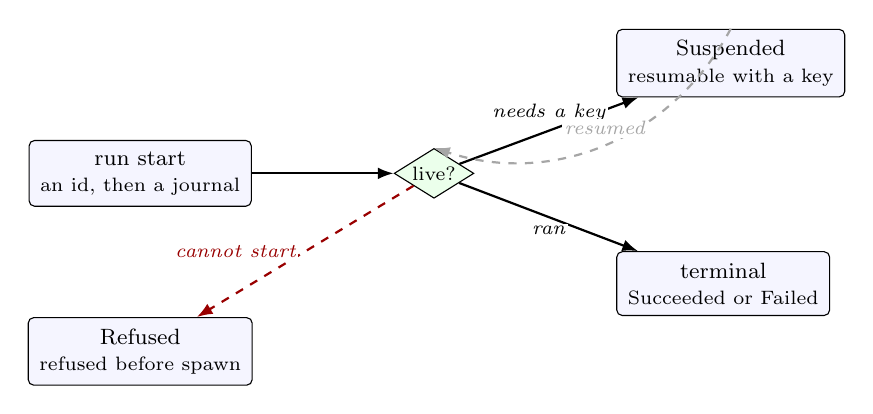
\begin{tikzpicture}[node distance=14mm and 18mm]
  \node[b] (start) {run start\\\scriptsize an id, then a journal};
  \node[v, right=of start] (live) {live?};
  \node[b, right=of live, yshift=14mm] (susp) {Suspended\\\scriptsize resumable with a key};
  \node[b, right=of live, yshift=-14mm] (term) {terminal\\\scriptsize Succeeded or Failed};
  \node[b, below=of start] (refused) {Refused\\\scriptsize refused before spawn};
  \draw[f] (start) -- (live);
  \draw[f] (live) -- node[p,above=2pt,midway]{needs a key} (susp);
  \draw[f] (live) -- node[p,below=2pt,midway]{ran} (term);
  \draw[sf] (susp.north) to[bend left=40] node[p,above=2pt,midway]{resumed} (live.north);
  \draw[bk] (live) -- node[p,left=2pt,midway]{cannot start} (refused);
\end{tikzpicture}}
\captionof{figure}{Five statuses, and the loop that matters: a suspended run is not a finished
one. Retention keeps a Running or Suspended run however old it is, because the daemon may still
resume it.}
\end{center}

A direct run reports one of three terminals, and \texttt{pii graph run} maps them to exit
codes an operator can branch on: success is 0, a failure is 1, a suspended run is 4, and a
graph the validator refuses is 3 --- before anything is executed and, deliberately, before
any store file is created.

\section{What it remembers, and where}

Seven store files appear in \texttt{pii health}. Six of them are what a backup copies:
the main store, memory, approvals, heal, channel and timer. The queue has its own file
and is reported alongside them, but it is not in the backup set at this revision --- a
detail that matters the first time you restore and find the work list empty.

\begin{center}
\resizebox{\linewidth}{!}{
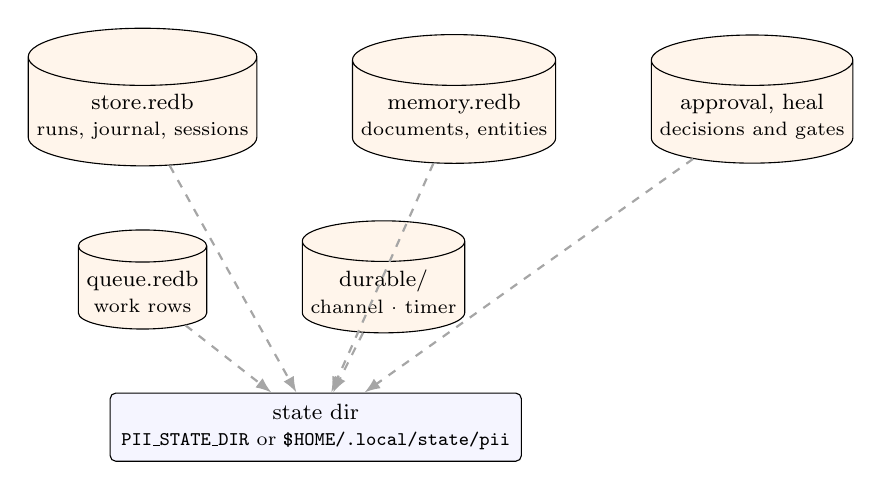
\begin{tikzpicture}[node distance=8mm and 12mm]
  \node[s] (main) {store.redb\\\scriptsize runs, journal, sessions};
  \node[s, right=of main] (mem) {memory.redb\\\scriptsize documents, entities};
  \node[s, right=of mem] (aux) {approval, heal\\\scriptsize decisions and gates};
  \node[s, below=of main] (q) {queue.redb\\\scriptsize work rows};
  \node[s, right=of q] (dur) {durable/\\\scriptsize channel \textperiodcentered{} timer};
  \node[b, below=of q, xshift=22mm] (dir) {state dir\\\scriptsize \texttt{PII\_STATE\_DIR} or
\texttt{\$HOME/.local/state/pii}};
  \draw[sf] (main) -- (dir);
  \draw[sf] (mem) -- (dir);
  \draw[sf] (aux) -- (dir);
  \draw[sf] (q) -- (dir);
  \draw[sf] (dur) -- (dir);
\end{tikzpicture}}
\captionof{figure}{Every store except the socket lives under one state directory. The durable
pair sits in \texttt{durable/} because the runtime directory is a tmpfs on a normal host, and a
channel cursor or a timer that vanishes at reboot is worse than no timer at all.}
\end{center}

The main store is a redb file, which never shrinks on its own: space is returned only at
the end of the file, and only by compaction. That is the reason a retention policy exists
at all, and the reason \texttt{pii store compact} is documented as narrow --- it reclaims
free pages inside the file, not live history.

\section{Capabilities are a ceiling}

Twelve capability bits exist, and every one of them is checked twice: the graph declares
what it may hold, and each node may hold only what its graph holds. A node that asks for
more is refused at load, not degraded at runtime.

\begin{center}
\resizebox{\linewidth}{!}{
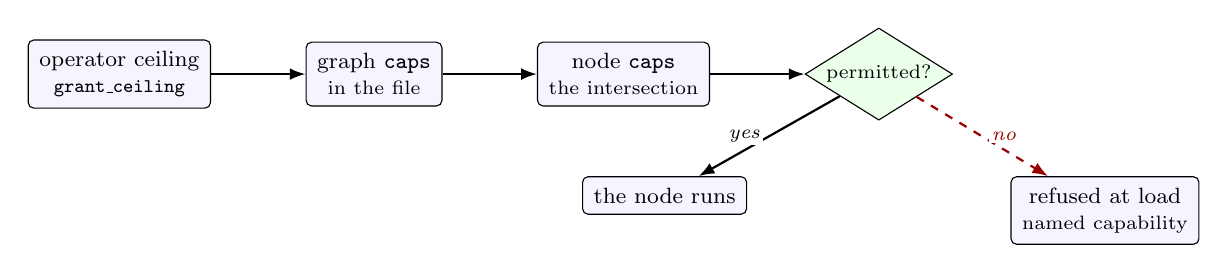
\begin{tikzpicture}[node distance=10mm and 12mm]
  \node[b] (ceiling) {operator ceiling\\\scriptsize \texttt{grant\_ceiling}};
  \node[b, right=of ceiling] (graph) {graph \texttt{caps}\\\scriptsize in the file};
  \node[b, right=of graph] (node) {node \texttt{caps}\\\scriptsize the intersection};
  \node[v, right=of node] (allow) {permitted?};
  \node[b, below left=of allow] (yes) {the node runs};
  \node[b, below right=of allow] (no) {refused at load\\\scriptsize named capability};
  \draw[f] (ceiling) -- (graph);
  \draw[f] (graph) -- (node);
  \draw[f] (node) -- (allow);
  \draw[f] (allow) -- node[p,left=2pt,midway]{yes} (yes);
  \draw[bk] (allow) -- node[p,right=2pt,midway]{no} (no);
\end{tikzpicture}}
\captionof{figure}{The ladder narrows downwards and never widens. A \texttt{call} can grant only
what its host grants, which is why \texttt{night} holds what \texttt{queue} needs before it may
call it.}
\end{center}

\begin{longtable}{@{}p{0.20\textwidth}p{0.72\textwidth}@{}}
	\toprule
	\textbf{Capability} & \textbf{What holding it allows} \\
	\midrule
	\endhead
	\texttt{fs\_read} & Read files inside an allow path scope. \\
	\texttt{fs\_write} & Write files inside an allow path scope. \\
	\texttt{proc} & Run commands --- this is what lets a judge execute exit criteria. \\
	\texttt{spawn} & Start an agent or a child process. Every model call needs it. \\
	\texttt{net} & Reach the network, subject to the config's host grants. \\
	\texttt{hw} & Touch hardware through the HAL. \\
	\texttt{secrets} & Read secret material. \\
	\texttt{memory\_read}, \texttt{memory\_write} & Read from, or write into, the agent's
	memory. \\
	\texttt{post} & Send a message into a configured channel. \\
	\texttt{mqtt\_read}, \texttt{mqtt\_write} & List and subscribe to a broker's devices;
	command one through its allowlist. \\
	\bottomrule
\end{longtable}

The measured consequence is worth stating plainly: a coder inside a graph whose
\texttt{caps} omitted \texttt{fs\_write} did not silently write nothing. It stopped and
reported \enquote{no write or execute tool is available}. That sentence is the feature
working; a degraded coder that pretends to work is the failure it replaced.

\section{How a run is named, and what a trace looks like}

Run identifiers are allocated by the store, not by the caller, so two processes cannot
collide: the daemon's own logs and the graph files quote them in the form
\texttt{r000000000130}. A caller may pass \texttt{--run-id} on the offline path, which is
how the test suites keep a fixture's journal findable.

\texttt{pii health} is the widest single view of what a process is. Its text form is
short enough to quote in a bug report, and every line is a fact a command can be held to:

\begin{lstlisting}[language=bash]
pii <version> (<revision>, <target>)
client: <revision>
config: <path> sha256=<hash>
stores:
  main: <path> (<bytes> bytes, format_version=<n>)
  memory: <path> (<bytes> bytes, format_version=<n>)
mounts:
  workspace [rw]: <root>  (<policy>)
since_deploy:
  starts: <n>
counts:
  runs: <n>
\end{lstlisting}

The field names, their order and their punctuation are exact; the values are whatever your
daemon reports. Read it as four claims, in order. The first line is \emph{what the daemon
is}: version, revision and target. The second is \emph{what your client is}: if the two
revisions differ, \texttt{pii health} exits 3 and prints a line beginning \texttt{DRIFT},
and that is the correct reading immediately after installing a new binary and before
restarting the service. The \texttt{config} line is the hash of the file the daemon actually
loaded --- not the path you think it loaded. The \texttt{stores} block is the one that
catches the most common installation mistake: a daemon whose store list is empty is a
daemon pointed at an empty directory, and it will happily report itself active.

\section{What pii refuses to claim}

Three refusals are part of the design, and an administrator meets all three.

\begin{itemize}
	\item A store whose format version is newer than the binary supports is not read
	half-way. The daemon exits 2 and writes nothing to the file, with the version and the
	path in the message.
	\item A health answer whose build revision is unknown on either side is reported as
	unverified, with a non-zero exit code, rather than as agreement. Unknown is never
	agreement.
	\item A retention sweep will not remove a row it cannot date. A run created before the
	clock was recorded, or a fixture with no timestamp, is kept and counted, because
	deleting on a missing timestamp destroys exactly the runs an operator is looking for.
\end{itemize}

\section{What it deliberately is not}

Four absences are decisions rather than gaps, and each one shapes how you operate the
thing.

\begin{itemize}
	\item \textbf{Not a cluster.} The stores are redb files with an exclusive lock, and the
	daemon claims the durable pair before it binds its socket. A second daemon pointed at
	the same state directory is refused, by name, at start. Scaling out means changing the
	store, not adding a replica.
	\item \textbf{Not an online compactor.} \texttt{pii store compact} runs redb's in-place
	compaction, and it needs the daemon stopped, because it takes the same exclusive lock
	the daemon holds for its lifetime. There is no background compaction to tune or to
	fear.
	\item \textbf{Not a cron daemon.} A \texttt{[[cron]]} entry carries a
	\texttt{schedule} string, but that string is a display mirror: what fires a graph is a
	\texttt{timer} node at its entry. A graph whose entry is not a timer will not be
	started by the schedule, and the config will look correct while nothing runs.
	\item \textbf{Not a TLS client for MQTT.} The broker client speaks plain TCP. A remote
	broker with credentials needs an explicit acknowledgement in the config, and the
	honest answer for a non-loopback broker is a tunnel.
\end{itemize}

Knowing these four saves the two most expensive mistakes in operation: pointing a second
process at a live state directory, and believing a schedule that only mirrors itself.

\section{How to read this manual}

Chapter~\ref{ch:install} gets a host running: the two directories, the installer, the
unit, the credentials, and the three commands that prove the result. Chapter~\ref{ch:daily}
is what a normal day looks like --- health, one-shot prompts, graphs by name and by file,
the queue, and how to read a trace. Chapter~\ref{ch:operate} is the part nobody reads
until something breaks: backup and restore, retention, upgrades, logs, disk ownership, the
deploy card and the failure modes that have actually happened.

Chapters~\ref{ch:commands} and~\ref{ch:config} are reference material and are meant to be
searched, not read. Chapter~\ref{ch:observability} is the metrics and event surface, and
Chapter~\ref{ch:graphs} is the graph library: which graphs an operator runs and what each
will do to the machine.

Two conventions run through the book. A path in \texttt{typewriter} is literal and was
copied from the repository or from a command's own output. A number in the text is a
measurement recorded in the repository, with the row or document that recorded it named
where the number is load-bearing. Where this manual and a design document disagree, the
manual is describing the code at the built revision, and the disagreement is itself worth
reporting.

\chapter{Installation}

\label{ch:install}

pii installs as a \emph{user} service by default. There is no package and, in that scope,
no root-owned state: the binary, its configuration, its graphs and its stores all live under
your own home, which is also what makes an upgrade a matter of replacing files that the
installer has already moved aside. A system scope exists --- \texttt{SCOPE=system}, with
\texttt{/etc/pii} and \texttt{/var/lib/pii} --- and everything below is written to be read
with either in mind. This chapter is the whole install path --- the two
directories, the script that fills them, the unit that supervises the process, the
credential file, and the commands that prove the result. It also lists the
preconditions the installer checks before it changes anything, because every one of them
was added after an install that half-succeeded.

\section{What you need}

\begin{itemize}
	\item a Linux host with a writable \texttt{\$HOME} and a user session. systemd
	\texttt{--user} is how the daemon is normally supervised, but it is not required: the
	daemon is a foreground process that can be started by hand, and on a host without a
	user bus that is the only way it runs;
	\item a kernel that can enforce the sandbox profile. Landlock is the mechanism; if the
	profile cannot be enforced the daemon \emph{refuses to start} with exit code 4 rather
	than falling back to unconfined;
	\item the \texttt{pii} binary, built for the host's architecture, plus the three
	sibling binaries if you want them;
	\item \texttt{curl}, which the installer uses for one precondition probe;
	\item Python 3.11 or newer with \texttt{tomllib}, which the installer uses to merge and
	verify the configuration file. The script locates it, or falls back to a \texttt{uv}
	provisioned interpreter under \texttt{\_tmp/};
	\item a provider credential for any workflow that calls a model. It is kept in the
	environment of the service, never in a file that is committed;
	\item a \emph{deploy card} for the revision you are about to install. It is a JSON file
        under \texttt{\_tmp/deploy/} named \texttt{card-\textless{}rev\textgreater{}.json},
keyed by the seven- or
	twelve-character short revision of \texttt{HEAD}. The installer refuses without one.
\end{itemize}

The deploy card is the one precondition that surprises people. It is not bureaucracy
around the install script: it is the record that a specific revision was proved red on
its base, green on its branch, gated, and rehearsed for rollback. A card is rendered,
approved or refused with \texttt{pii deploy-card}, and a card missing any of its five
fields is refused with the field named and no approval path printed.

\section{The binary and the state directory}

The binary is self-contained. Its \emph{state} lives in a directory chosen once, by one
function, in this order:

\begin{enumerate}
	\item \texttt{PII\_STATE\_DIR}, when set and non-empty;
	\item otherwise \texttt{\$HOME/.local/state/pii}.
\end{enumerate}

That single resolver is deliberate. Before it, several commands each had their own notion
of where the store lived, and a command could read a store the daemon was not writing.
The measured symptom was not a crash: it was a CLI reporting an empty run list while the
daemon served hundreds of runs from another file. If you set \texttt{PII\_STATE\_DIR} for
a test, set it for the daemon too, or you are looking at two different systems.

The \emph{runtime} directory is a second, separate rule, and mixing the two up is the most
common installation defect:

\begin{enumerate}
	\item \texttt{PII\_RUNTIME\_DIR}, when set;
	\item \texttt{[core].runtime\_dir} from the config file;
	\item \texttt{/run/user/\textless{}uid\textgreater{}/pii}.
\end{enumerate}

The runtime directory holds the control socket and, on a normal host, is a tmpfs. That is
why the durable stores --- the channel cursor and the timer wheel --- default to
\texttt{\textless{}state dir\textgreater{}/durable} and never to the runtime directory: a timer
that disappears at
reboot is worse than no timer at all. It is also why the installer symlinks the graphs
directory into the runtime directory on every start rather than copying it there.

\subsection*{The shape of an installation}

\begin{center}
\resizebox{\linewidth}{!}{
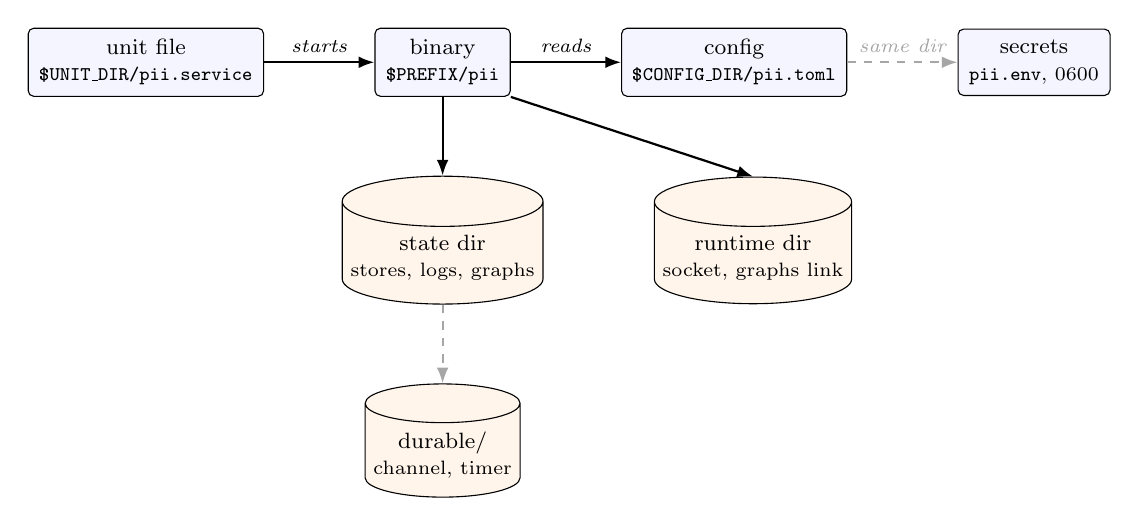
\begin{tikzpicture}[node distance=10mm and 14mm]
  \node[b] (unit) {unit file\\\scriptsize \texttt{\$UNIT\_DIR/pii.service}};
  \node[b, right=of unit] (bin) {binary\\\scriptsize \texttt{\$PREFIX/pii}};
  \node[b, right=of bin] (conf) {config\\\scriptsize \texttt{\$CONFIG\_DIR/pii.toml}};
  \node[b, right=of conf] (env) {secrets\\\scriptsize \texttt{pii.env}, 0600};
  \node[s, below=of bin] (state) {state dir\\\scriptsize stores, logs, graphs};
  \node[s, right=of state] (run) {runtime dir\\\scriptsize socket, graphs link};
  \node[s, below=of state] (dur) {durable/\\\scriptsize channel, timer};
  \draw[f] (unit) -- node[p,above=2pt,midway]{starts} (bin);
  \draw[f] (bin) -- node[p,above=2pt,midway]{reads} (conf);
  \draw[sf] (conf) -- node[p,above=2pt,midway]{same dir} (env);
  \draw[f] (bin.south) -- (state.north);
  \draw[f] (bin.south east) -- (run.north);
  \draw[sf] (state) -- (dur);
\end{tikzpicture}}
\captionof{figure}{What an installation owns, in the user scope. Notice the two dashed edges:
the key file sits beside the config but is read by the service, and the unit is only a file
until an operator enables it.}
\end{center}

\section{The installer, stage by stage}

One command does the whole install, and it is idempotent. It never deletes: anything it
replaces is moved into a dated directory first, so a failed install leaves you able to
compare and to roll back.

\begin{lstlisting}[language=bash]
bash deploy/install-pii.sh                    # SCOPE=user (the default)
SCOPE=system bash deploy/install-pii.sh       # /etc/systemd/system, /etc/pii, /var/lib/pii
CONFIG_ONLY=1 bash deploy/install-pii.sh      # rewrite the config and credentials only
\end{lstlisting}

The stages run in a fixed order, and the preconditions are all checked before the first
file moves. That ordering is not cosmetic: it means an aborted install changes nothing,
which is the only property that makes a script safe to run on a host you care about. The
one exception is \texttt{CONFIG\_ONLY=1}, which skips the build, the card, the binaries and
the unit, and touches only the config file and the credential file.

\begin{center}
\resizebox{\linewidth}{!}{
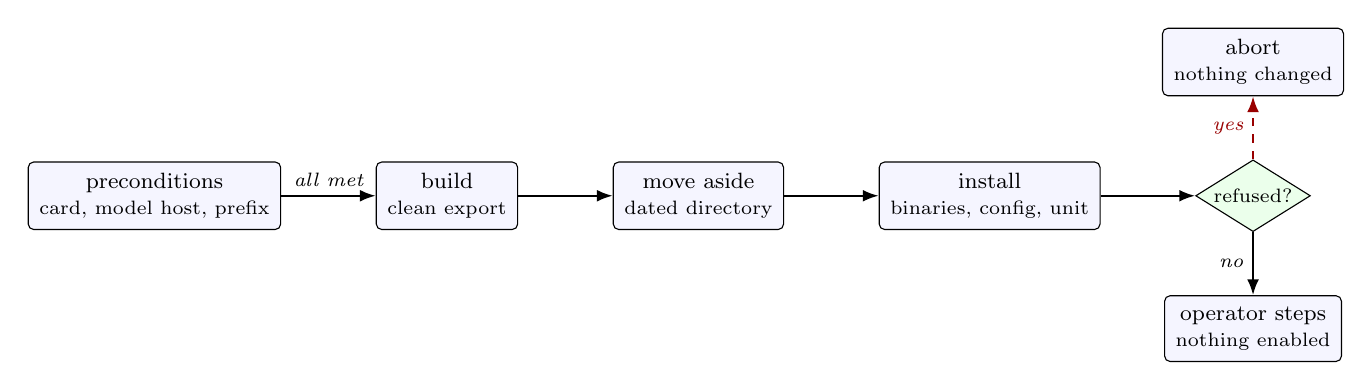
\begin{tikzpicture}[node distance=8mm and 12mm]
  \node[b] (pre) {preconditions\\\scriptsize card, model host, prefix};
  \node[b, right=of pre] (build) {build\\\scriptsize clean export};
  \node[b, right=of build] (move) {move aside\\\scriptsize dated directory};
  \node[b, right=of move] (install) {install\\\scriptsize binaries, config, unit};
  \node[v, right=of install] (ok) {refused?};
  \node[b, above=of ok] (abort) {abort\\\scriptsize nothing changed};
  \node[b, below=of ok] (print) {operator steps\\\scriptsize nothing enabled};
  \draw[f] (pre) -- node[p,above=2pt,midway]{all met} (build);
  \draw[f] (build) -- (move);
  \draw[f] (move) -- (install);
  \draw[f] (install) -- (ok);
  \draw[bk] (ok) -- node[p,left=2pt,midway]{yes} (abort);
  \draw[f] (ok) -- node[p,left=2pt,midway]{no} (print);
\end{tikzpicture}}
\captionof{figure}{The installer's shape. Every refusal happens either before the build or in
the config-merge step, which restores the replaced file byte for byte. The script ends by
printing what an operator still has to do; it never enables or starts the unit.}
\end{center}

\subsection*{What the preconditions cost when they fail}

Each precondition exists because the failure it prevents was measured.

\begin{itemize}
	\item \textbf{The model host must answer.} The script does
        \texttt{GET \textless{}llama host\textgreater{}/models} with a five-second limit and
aborts if it does not.
	Without this probe an install succeeds and every graph that needs a model fails at
	spawn, minutes later, with the daemon looking healthy.
	\item \textbf{The named graphs must exist.} The generated configuration names
	\texttt{discord-triage} and \texttt{discord-digest}; the script refuses if either file
	is missing from \texttt{graphs/}, because a config that names a graph the daemon cannot
	load is a daemon that starts with a channel and no work.
	\item \textbf{The prefix must be writable.} It is created if absent and refused if it
	cannot be written --- before the build, so a permissions problem costs seconds rather
	than a release compile.
	\item \textbf{The working tree must be a git checkout.} The card is keyed by the short
	revision of \texttt{HEAD}, and there is no install without a card.
\end{itemize}

The build itself is worth one paragraph, because two deployment defects are recorded in
its comments. The script exports \texttt{git archive HEAD} into a temporary directory and
builds there. Measured on three consecutive deploys, building in the working tree shipped
binaries that reported \texttt{\textless{}rev\textgreater{}-dirty} whenever any path was
uncommitted --- including
a worker's leftover --- so the revision the deploy card quotes carried a suffix meaning
\emph{this is not the commit you verified}. The export has no \texttt{.git}, so
\texttt{build.rs} cannot read the revision from it; the script therefore passes
\texttt{PII\_BUILD\_REVISION} explicitly. That was measured too: the first export-built
binary reported \texttt{unknown} for a build correctly made from a known commit, and
\texttt{pii health} classified it as unverified for ever after.

\section{Environment and scope}

Every path the installer writes is an environment variable with a default, so a second
installation on the same host --- a test prefix, a different user --- needs no editing of
the script.

\begin{longtable}{@{}p{0.20\textwidth}p{0.36\textwidth}p{0.40\textwidth}@{}}
	\toprule
	\textbf{Variable} & \textbf{User scope default} & \textbf{System scope default} \\
	\midrule
	\endhead
	\texttt{SCOPE} & \texttt{user} & \texttt{system} \\
	\texttt{PREFIX} & \texttt{\$HOME/.local/bin} & \texttt{\$HOME/.local/bin} (the static
	unit in \texttt{deploy/} instead names \texttt{/usr/local/bin/pii}) \\
	\texttt{CONFIG\_DIR} & \texttt{\$HOME/.config/pii} & \texttt{/etc/pii} \\
	\texttt{STATE\_DIR} & \texttt{\$HOME/.local/state/pii} & \texttt{/var/lib/pii} \\
	\texttt{RUNTIME\_DIR} & \texttt{/run/user/\textless{}uid\textgreater{}/pii} & \texttt{/run/pii} \\
	\texttt{UNIT\_DIR} & \texttt{\$HOME/.config/systemd/user} & \texttt{/etc/systemd/system} \\
	\texttt{BIN\_SRC} & \texttt{\textless{}repo\textgreater{}/target/release} & same \\
	\texttt{LLAMA\_HOST} & \texttt{http://10.10.10.217:8082/v1} & same \\
	\bottomrule
\end{longtable}

Three more variables change what the script does rather than where it writes.
\texttt{SKIP\_BUILD=1} installs the binaries already in \texttt{BIN\_SRC} and is how a
host without a Rust toolchain takes a release;
\texttt{CONFIG\_ONLY=1} rewrites only the configuration and the channel credentials, with
no build, no card, no binaries and no unit, which is the supported way to change a model
host or a token on a running installation; and \texttt{PII\_PYTHON} pins the interpreter
used for the config merge.

\section{The configuration file}

Behaviour lives in one TOML file, and the file is strict: an unknown key is a load
error, so a typo in a sandbox or a runtime path cannot silently become a default. The
installer writes it by \emph{merging} rather than regenerating, and then verifies that
every table and key path of the replaced file is present in the candidate, naming each
miss instead of proceeding. Before that change, a re-install rewrote the file from the
template and carried only \texttt{model} forward --- which is how an operator's sections
disappeared.

The sections the daemon reads are these, and nothing else:

\begin{center}
\begin{tabular}{@{}p{0.22\textwidth}p{0.66\textwidth}@{}}
	\toprule
	\textbf{Section} & \textbf{What it decides} \\
	\midrule
	\texttt{grant\_ceiling} (top level) & the capability names no graph or node may request
	beyond; empty means no ceiling \\
	\texttt{[core]} & model, runtime dir, durable dir, log file and rotation, trajectory
	root and its bounds, the measurement switches \\
	\texttt{[llama]} & the base URL a \texttt{llamacpp-server:} model dials \\
	\texttt{[net]} & egress host patterns and whether private destinations are allowed \\
	\texttt{[memory]}, \texttt{[memory\_graph]} & the memory store's path and graph
	settings \\
	\texttt{[[worker]]} & supervised child processes, with their own in-flight limits \\
	\texttt{[[channel]]} & inbound message sources and the graph each message runs \\
	\texttt{[[mqtt]]} & broker connections, topics and the graph per message \\
	\texttt{[[cron]]} & named schedules, and the graph each one names \\
	\texttt{[hal]}, \texttt{[wasm]}, \texttt{[evolve]} & optional subsystems; absent means
	off \\
	\texttt{[[model\_tier]]} & named model tiers \\
	\bottomrule
\end{tabular}
\end{center}

The \texttt{[core]} keys an administrator actually touches are
\texttt{model}, \texttt{runtime\_dir}, \texttt{durable\_dir}, \texttt{log\_file},
\texttt{log\_rotate\_bytes} (default 10485760), \texttt{log\_keep\_files} (default 5),
\texttt{trajectory\_dir} (absent means trajectories are off),
\texttt{trajectory\_max\_bytes} (default 512 MiB), \texttt{trajectory\_max\_files}
(default 50\,000), and the two measurement switches \texttt{observer} and \texttt{audit},
which default to \texttt{on} and must stay on in production.

\subsection*{The path the CLI reads is not always the path the service reads}

\texttt{pii daemon} takes \texttt{--config}, defaulting to \texttt{\$PII\_CONFIG} and then
\texttt{\$HOME/.pii/pii.toml}. The installer writes \texttt{\$CONFIG\_DIR/pii.toml} ---
\texttt{\$HOME/.config/pii/pii.toml} in the user scope --- and puts
\texttt{PII\_CONFIG} in the unit. The consequence is exact and worth memorising: a shell
that runs \texttt{pii} without \texttt{PII\_CONFIG} set is reading a different file from
the one the daemon loaded, and \texttt{pii health} will show you the daemon's file by
path and hash if you ask. Export \texttt{PII\_CONFIG} in your shell, or accept that the
two are separate.

The same shape applies to the store. \texttt{pii daemon --help} documents the default as
\texttt{\textless{}runtime dir\textgreater{}/store.redb}, while the store commands and the
backup default to the
state directory; the change that would make the daemon agree had not landed at this
revision. Do what the shipped unit does: pass \texttt{--store} explicitly, pointing at
\texttt{\$STATE\_DIR/store.redb}.

\section{Credentials}

Model providers and channels are reached with values taken from the environment of the
process that needs them. Nothing in the configuration file is a secret, and no pii command
prints one: provider errors and events are scrubbed of the key before they are written.

The convention in this deployment is a single environment file next to the config,
owned by the user, mode \texttt{0600}, read by the service unit and never by the
repository:

\begin{lstlisting}[language=bash]
install -m 600 /dev/null ~/.config/pii/pii.env
# then edit it to hold the provider key(s) and the channel ids, and nothing else
chmod 600 ~/.config/pii/pii.env
\end{lstlisting}

The unit reference is written with a leading dash ---
\texttt{EnvironmentFile=-\$CONFIG\_DIR/pii.env} --- which makes the file optional. The
difference matters: without the dash, a missing file is a unit that fails to start, and the
error is about systemd rather than about the credential. With it, the daemon starts and
reports what it does not have --- \texttt{channels: []} --- which is a state to report, not
a failure to diagnose.

\begin{center}
\resizebox{\linewidth}{!}{
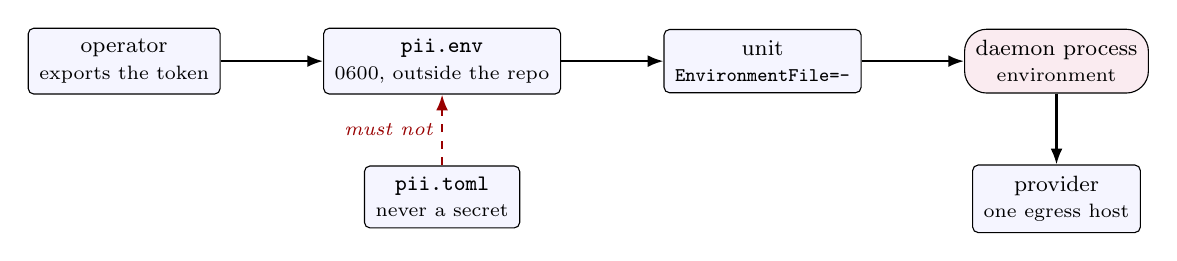
\begin{tikzpicture}[node distance=9mm and 13mm]
  \node[b] (ops) {operator\\\scriptsize exports the token};
  \node[b, right=of ops] (envf) {\texttt{pii.env}\\\scriptsize 0600, outside the repo};
  \node[b, right=of envf] (unit) {unit\\\scriptsize \texttt{EnvironmentFile=-}};
  \node[m, right=of unit] (proc) {daemon process\\\scriptsize environment};
  \node[b, below=of proc] (provider) {provider\\\scriptsize one egress host};
  \node[b, below=of envf] (conf) {\texttt{pii.toml}\\\scriptsize never a secret};
  \draw[f] (ops) -- (envf);
  \draw[f] (envf) -- (unit);
  \draw[f] (unit) -- (proc);
  \draw[f] (proc) -- (provider);
  \draw[bk] (conf) -- node[p,left=2pt,midway]{must not} (envf);
\end{tikzpicture}}
\captionof{figure}{The secret path. The value reaches the daemon's environment and nothing else;
the config file names the shape of the connection, never the credential. A key pasted into a
chat or a commit is compromised, and rotation is the only remedy.}
\end{center}

Named variables, so a grep for one of them in the tree is a finding: \texttt{OPENAI\_API\_KEY}
and \texttt{OPENAI\_BASE\_URL}; \texttt{ANTHROPIC\_API\_KEY} and
\texttt{ANTHROPIC\_BASE\_URL}; \texttt{GEMINI\_API\_KEY} and \texttt{GEMINI\_BASE\_URL};
\texttt{PII\_MODEL} for a default model; \texttt{PII\_DISCORD\_TOKEN} and
\texttt{PII\_DISCORD\_CHANNEL\_ID} for the one forum channel the installer configures.
Egress is granted per host: the daemon grants \texttt{http:\textless{}host\textgreater{}} for
the host of the
configured base URL only, and any other host is denied and reported.

\section{Supervising the daemon}

The daemon is a foreground process: \texttt{--foreground} is accepted for supervisors and
changes nothing, because the daemon never forks. The installer writes this unit and does
not enable it:

\begin{lstlisting}
[Unit]
Description=Pii daemon
After=network-online.target

[Service]
Type=simple
$USERLINE
Environment=PII_RUNTIME_DIR=$RUNTIME_DIR
Environment=PII_CONFIG=$CONF
EnvironmentFile=-$CONFIG_DIR/pii.env
WorkingDirectory=$STATE_DIR
ExecStartPre=/usr/bin/env mkdir -p $RUNTIME_DIR
ExecStartPre=/usr/bin/env ln -sfn $STATE_DIR/graphs $RUNTIME_DIR/graphs
ExecStart=$PREFIX/pii daemon --foreground --config $CONF --store $STATE_DIR/store.redb \
  --workspace $STATE_DIR --log-file $STATE_DIR/pii.log \
  --log-rotate-bytes 10485760 --log-keep-files 5
Restart=always
RestartSec=2
TimeoutStopSec=10
NoNewPrivileges=yes

[Install]
WantedBy=$WANTED
\end{lstlisting}

The variables are the installer's own: \texttt{\$USERLINE} is a \texttt{User=} line and is
emitted only in the system scope, and \texttt{\$WANTED} is \texttt{default.target} for a
user unit and \texttt{multi-user.target} for a system one.

Two lines in that unit are load-bearing beyond the obvious. The symlink of the graphs
directory runs on every start because the runtime directory is a tmpfs: the graphs live in
the state directory and are placed where the daemon looks for them at each boot.
\texttt{TimeoutStopSec=10} matches the daemon's own shutdown: it waits at most five seconds
for in-flight blocking work, then exits anyway, so a stop that needs more than ten seconds
is a stuck process and systemd will kill it.

Then enable it, and make it survive logout if the host is meant to run unattended:
\texttt{systemctl --user daemon-reload}, then \texttt{systemctl --user enable --now pii},
then \texttt{loginctl enable-linger} for the account. Nothing in the installer runs those
three commands, which is deliberate --- an install that starts a service is an install you
cannot inspect before it acts.

The repository also ships a static unit for the system scope,
\texttt{deploy/pii.service}, which uses \texttt{DynamicUser=yes} with
\texttt{StateDirectory}, \texttt{RuntimeDirectory} and \texttt{LogsDirectory} so that
\texttt{/var/lib/pii}, \texttt{/run/pii} and \texttt{/var/log/pii} are created, owned and
kept across restarts. Use one or the other, not both: two units for the same daemon is the
same defect as two daemons for the same store.

\section{The graphs an installation serves}

Graphs are installed as files under \texttt{\$STATE\_DIR/graphs}, and the daemon resolves
a name through three directories in order: \texttt{\textless{}runtime dir\textgreater{}/graphs},
then the
\texttt{graphs} directory beside the store, then
\texttt{\$HOME/.local/state/pii/graphs}. A directory listed twice is searched once. That
order is why an installed copy can shadow a repository copy, and why
\texttt{pii graph list} prints a drift column: \texttt{same}, \texttt{DRIFT},
\texttt{installed-only} or \texttt{repo-only} compares each installed file against its
repository twin by the hash of its bytes.

\begin{lstlisting}[language=bash]
pii graph list                  # name, hash, node count, trigger, armed runs, drift
pii graph list --all            # include graphs that are only in the repository
pii graph edit queue --file graphs/queue.toml    # lint, move the old one aside, write atomically
\end{lstlisting}

\texttt{pii graph edit} never deletes a graph: it lints the candidate first, moves the
previous file aside, and writes atomically. A graph that fails lint is not installed at
all, so a bad edit cannot take out a working graph.

\section{Verifying the installation}

Four commands, in increasing depth. Each has an expected reading, and the exit codes are
part of the answer.

\begin{lstlisting}[language=bash]
pii --version                 # the binary you are actually running
pii health                    # 0 = this build, 2 = no daemon, 3 = drift or unverified
pii health --json             # the full sys.status payload, for a script
pii graph list                # does the daemon see the graphs on disk?
\end{lstlisting}

\begin{center}
\resizebox{\linewidth}{!}{
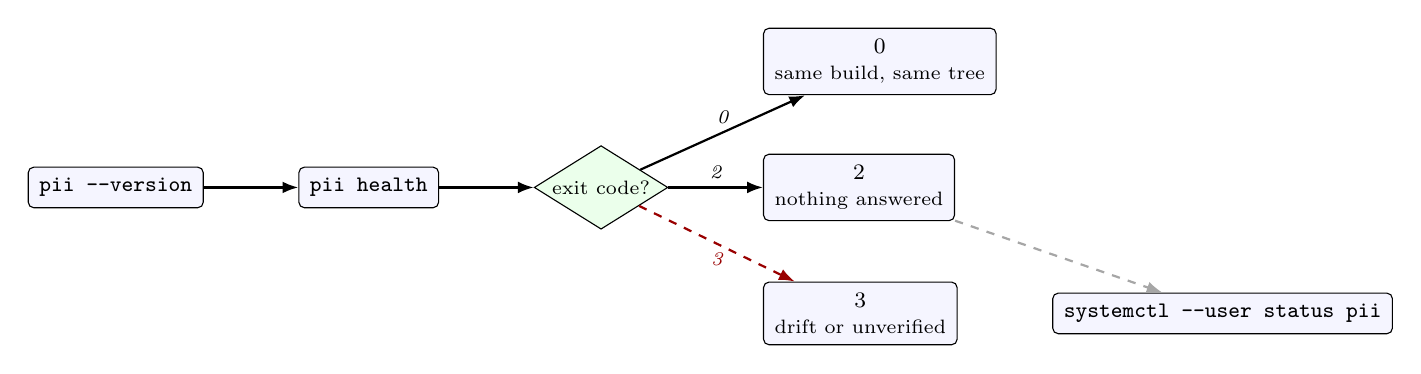
\begin{tikzpicture}[node distance=12mm and 12mm]
  \node[b] (v) {\texttt{pii --version}};
  \node[b, right=of v] (h) {\texttt{pii health}};
  \node[v, right=of h] (code) {exit code?};
  \node[b, right=of code, yshift=16mm] (zero) {0\\\scriptsize same build, same tree};
  \node[b, right=of code] (two) {2\\\scriptsize nothing answered};
  \node[b, right=of code, yshift=-16mm] (three) {3\\\scriptsize drift or unverified};
  \node[b, right=of three] (unit) {\texttt{systemctl --user status pii}};
  \draw[f] (v) -- (h);
  \draw[f] (h) -- (code);
  \draw[f] (code) -- node[p,above=2pt,midway]{0} (zero);
  \draw[f] (code) -- node[p,above=2pt,midway]{2} (two);
  \draw[bk] (code) -- node[p,below=2pt,midway]{3} (three);
  \draw[sf] (two) -- (unit);
\end{tikzpicture}}
\captionof{figure}{The verification ladder, and the three readings of \texttt{pii health}. Exit
3 immediately after an install is correct: the client is the new binary and the daemon is still
the old process. It becomes 0 only after the restart.}
\end{center}

A health answer whose \texttt{stores} list is empty is not a healthy daemon, whatever its
exit code: it is a daemon pointed at an empty directory. Check
\texttt{PII\_STATE\_DIR} and the unit's \texttt{--store} argument before believing anything
else. The same reading applies to \texttt{format\_version}: a store at a version the binary
does not know is refused at open, with the path and both versions in the message, and
nothing is written to the file.

\section{Rolling an installation back}

\texttt{deploy/rollback-pii.sh} undoes the last install without deleting anything. It
stops the unit if it is running, finds the newest
\texttt{\$PREFIX.old-\textless{}epoch\textgreater{}} directory,
and moves its contents back --- binaries to the prefix, \texttt{pii.toml} to the config
directory, the unit to the unit directory, and any \texttt{graph.*} file to the state
directory's \texttt{graphs}. Whatever it replaces is moved to
\texttt{\$PREFIX.rolledback-\textless{}epoch\textgreater{}}, and it prints each file restored.

\begin{lstlisting}[language=bash]
bash deploy/rollback-pii.sh
systemctl --user daemon-reload && systemctl --user restart pii
pii health                                    # back to the older revision, exit 0
\end{lstlisting}

The script is exercised in a scratch prefix by the deployment checks, and the drill is
worth repeating once on a real host before you need it: an install followed by a rollback
followed by \texttt{pii health} returning 0 proves both directions, and costs a minute.

\section{Failure modes of the install itself}

\begin{center}
\begin{tabular}{@{}p{0.34\textwidth}p{0.58\textwidth}@{}}
	\toprule
	\textbf{Symptom} & \textbf{Cause, and what to check} \\
	\midrule
	\texttt{ABORT: no deploy card for revision \ldots} & No
        \texttt{\_tmp/deploy/card-\textless{}rev\textgreater{}.json} for \texttt{HEAD}. Render
and approve a card, or
	install a revision that has one. \\
	\texttt{ABORT: llama.cpp host \ldots\ does not answer} & The model host is down or the
	URL is wrong. Nothing was changed; the probe runs before the build. \\
	\texttt{cargo: command not found} inside the export & A non-interactive shell did not
	carry your \texttt{PATH}. The script now exports it itself; an older copy of the script
	is what fails here. \\
        The installed binary reports \texttt{\textless{}rev\textgreater{}-dirty} & It was built
in the working tree.
	Only a clean-export build is deployable evidence. \\
	The installed binary reports \texttt{unknown} & The export build did not receive
	\texttt{PII\_BUILD\_REVISION}. Rebuild with the script, not by hand. \\
	\texttt{pii health} exits 2 after install & The unit was written but not enabled, or it
	failed to start. \texttt{systemctl --user status pii}, then the log file. \\
	The daemon starts but every graph fails at spawn & The model id is one the provider does
	not serve, or the key is not in the unit's environment. \\
	\bottomrule
\end{tabular}
\end{center}

The last row is the one that looks like a pii bug and usually is not. A model id that the
provider has retired fails at spawn, in a second, with no partial output; the spec graph
takes its \texttt{err} edge to a \texttt{refuse} node, and the queue records the row as
refused rather than failed. Read the id in the graph, then the model the daemon resolved,
then the provider's own list.

\chapter{Daily use}

\label{ch:daily}

A normal day with pii is short. You ask the daemon what it is, you give it work --- a
prompt, a graph, a queue row --- and then you read what it did. This chapter is that loop
in the order you actually run it, with the exact flags the binary accepts at the revision
this manual describes, the exit code each command returns, and the places where the answer
looks like a success and is not. Nothing here needs the repository; everything here assumes
a daemon that is already running, as installed in Chapter~\ref{ch:install}.

\begin{center}
\resizebox{\linewidth}{!}{
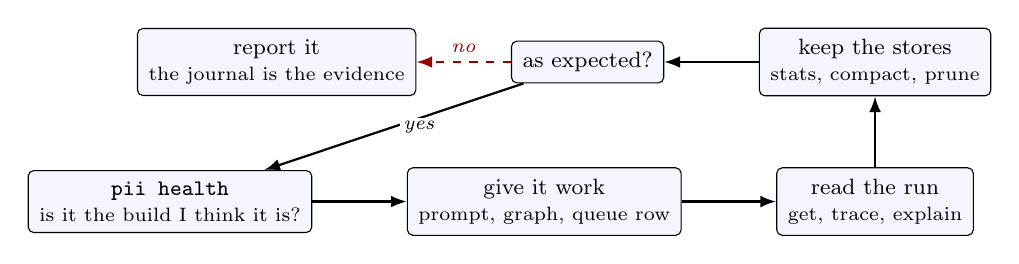
\begin{tikzpicture}[node distance=9mm and 12mm]
  \node[b] (health) {\texttt{pii health}\\\scriptsize is it the build I think it is?};
  \node[b, right=of health] (work) {give it work\\\scriptsize prompt, graph, queue row};
  \node[b, right=of work] (read) {read the run\\\scriptsize get, trace, explain};
  \node[b, above=of read] (keep) {keep the stores\\\scriptsize stats, compact, prune};
  \node[b, left=of keep] (fine) {as expected?};
  \node[b, left=of fine] (report) {report it\\\scriptsize the journal is the evidence};
  \draw[f] (health) -- (work);
  \draw[f] (work) -- (read);
  \draw[f] (read) -- (keep);
  \draw[f] (keep) -- (fine);
  \draw[bk] (fine) -- node[p,above=2pt,midway]{no} (report);
  \draw[f] (fine) -- node[p,right=2pt,midway]{yes} (health);
\end{tikzpicture}}
\captionof{figure}{The daily loop. The first and last steps are the ones that get skipped: a
health call before you trust a result, and a store reading before the disk tells you.}
\end{center}

\section{Asking the daemon a question}

\texttt{pii health} is the first command of any session, including a session that starts
with \enquote{it worked yesterday}. It prints the daemon's own account of itself and
returns an exit code that a script can branch on.

\begin{lstlisting}[language=bash]
pii health                 # human text; 0 = same build, 2 = no daemon, 3 = drift
pii health --json          # the sys.status payload, verbatim
pii metrics                # one name-value line per metric
pii disk                   # artefact roots with size, age and filesystem
\end{lstlisting}

The text form is documented line by line in Chapter~\ref{ch:what} and is not repeated
here. The useful habit is narrower: read \texttt{client:} against the first line, because
that pair is the only thing in pii that tells you whether the binary in your shell and the
process answering you are the same program. A \texttt{DRIFT} line on stderr with exit 3 is
not an error to fix; it is a fact to act on --- restart the service, or use the binary the
daemon is running.

\texttt{pii disk} answers a different question, and it exists because the answer used to
take four commands and a guess. It walks a fixed list of artefact roots
(\texttt{\_tmp/gate-target}, \texttt{\_tmp/gate-target-fresh}, \texttt{\_tmp/targets},
\texttt{\_tmp/\_trash}, \texttt{/projects/\_tmp}, \texttt{/projects/\_trash},
\texttt{/tmp/\_trash-podman}, \texttt{/tmp/gate-cache} and every unclaimed
\texttt{\_tmp/*target*} directory), prints each one's size, age, filesystem and
whether an owner claims it, then prints free space for \texttt{/} and for the volume that
holds the repository. It is read-only; removal is \texttt{cargo xtask disk --gc}, which
owns the TTL.

The reason it prints \emph{two} free-space lines is a measured defect: the gate's floor
was evaluated on \texttt{/} while the artefacts landed on \texttt{/projects}, so a host
with 16\,GB free on a 288\,GB overlay and 147\,GB free on the repository volume refused to
run --- and the obvious first move, \texttt{cargo clean} on the repository, freed space on
the volume that was never short.

\section{One-shot prompts}

\texttt{pii -p} is the shortest path to a model. It carries a prompt, and its flags decide
which model, which graph, which workspace and how much confinement.

\begin{lstlisting}[language=bash]
pii -p "summarise the open items in specs/350-an-incident-becomes-a-case.md"
pii -p "why did run r000000000130 end unverified" --model llamacpp-server:granite-4.2-3b
pii -p "check the tree" --graph preflight --workspace /projects/pi-improved
\end{lstlisting}

\begin{longtable}{@{}p{0.20\textwidth}p{0.72\textwidth}@{}}
	\toprule
	\textbf{Flag} & \textbf{Effect} \\
	\midrule
	\endhead
	\texttt{--model M} & the model spec for this call; wins over \texttt{\$PII\_MODEL} and
	over \texttt{[core].model} \\
	\texttt{--graph G} & run an installed graph instead of the default one-shot path \\
	\texttt{--workspace D} & the directory the sandbox and the tools are scoped to;
	defaults to the current directory \\
	\texttt{--sandbox off|workspace} & \texttt{workspace} is the default; \texttt{off}
	runs unconfined and says so \\
        \texttt{--connect auto|loopback|\textless{}socket\textgreater{}} & which transport to
use; \texttt{auto} takes
	a live daemon socket if one answers \\
	\texttt{--json} & machine-readable output; already the default when stdout is not a
	terminal \\
	\texttt{--input J} & extra graph input, merged into the run input as JSON \\
	\bottomrule
\end{longtable}

Two behaviours are easy to observe and worth knowing before the first surprise. The
transport is chosen for you: a live daemon socket wins, and only if nothing answers does
the command build the engine in its own process. The daemon is never started for you ---
there is no auto-start anywhere in the path --- so a \texttt{-p} on a host whose service is
down silently becomes an in-process engine with its own view of the state directory. And
if no model resolves at all, the command exits 5 with one line:
\enquote{no model configured (set PII\_MODEL or --model)}. That is a different failure from
a model the provider does not serve, which fails later, at spawn.

\section{Running a graph}

There are two ways to run a graph, and they are not interchangeable. By \emph{name}, you
ask the daemon, which serves the installed set and owns the stores. By \emph{file}, you run
it yourself against a store you name, which is what the test suites and a one-off
diagnostic do.

\begin{lstlisting}[language=bash]
# by name: the daemon resolves it, runs it, and journals it
pii run start queue --input '{"workdir":"/projects/pi-improved","base":"<40-hex>"}'

# by file: you own the store path and the write grants
pii graph run graphs/preflight.toml --db ~/.local/state/pii/store.redb \
  --input '{}' --allow-write /projects/pi-improved/_tmp
\end{lstlisting}

\begin{center}
\resizebox{\linewidth}{!}{
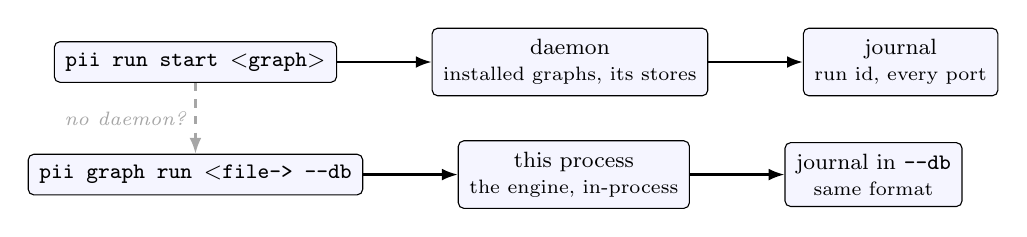
\begin{tikzpicture}[node distance=9mm and 12mm]
  \node[b] (name) {\texttt{pii run start \textless{}graph\textgreater{}}};
  \node[b, right=of name] (daemon) {daemon\\\scriptsize installed graphs, its stores};
  \node[b, right=of daemon] (journal) {journal\\\scriptsize run id, every port};
  \node[b, below=of name] (file) {\texttt{pii graph run \textless{}file-> --db}};
  \node[b, right=of file] (local) {this process\\\scriptsize the engine, in-process};
  \node[b, right=of local] (journal2) {journal in \texttt{--db}\\\scriptsize same format};
  \draw[f] (name) -- (daemon);
  \draw[f] (file) -- (local);
  \draw[f] (daemon) -- (journal);
  \draw[f] (local) -- (journal2);
  \draw[sf] (name) -- node[p,left=2pt,midway]{no daemon?} (file);
\end{tikzpicture}}
\captionof{figure}{Two paths, one journal format. The name path is what an installation uses;
the file path is what a diagnostic uses, and it is the only one where you choose the store.}
\end{center}

The offline path builds its own capability root, and the defaults are worth memorising
because they explain most \enquote{permission denied} results from a hand-run graph:
reads are allowed for the current directory, writes are allowed for
\texttt{\textless{}cwd\textgreater{}/\_tmp} plus every \texttt{--allow-write} directory, and the
only process
argv[0] permitted is \texttt{/bin/sh}. Everything else is denied by the capability check
before the node runs. \texttt{--allow-write} is canonicalised, so a relative or symlinked
grant would otherwise grant nothing.

Both paths share one exit-code vocabulary, and the two codes that are not 0 or 1 are the
interesting ones:

\begin{center}
\begin{tabular}{@{}p{0.10\textwidth}p{0.78\textwidth}@{}}
	\toprule
	\textbf{Code} & \textbf{Meaning} \\
	\midrule
	0 & the run reached its terminal node and reported success \\
	1 & the run failed, or could not be started; the message names the reason \\
	2 & usage error: an unknown flag, a missing value, \texttt{--input} that is not JSON \\
	3 & the validator refused the graph --- and, on this path, no store file was created \\
	4 & the run suspended and holds a resume key \\
	\bottomrule
\end{tabular}
\end{center}

The distinction between 3 and 1 is the reason a refused graph creates no store file: the
graph is loaded and validated \emph{before} the store is opened, so a wrong pin or a
missing callee costs nothing and leaves nothing behind.

\section{The queue}

The queue is how pii is given work rather than a question. A row carries an id, a title, a
spec path, the criteria that decide whether the work is done, and the paths the row expects
to touch. Every subcommand is one protocol call; none opens the store.

\begin{lstlisting}[language=bash]
pii queue add --id 376 --title "retention drops what the policy expires" \
  --spec /projects/pi-improved/specs/376-retention-drops-what-the-policy-expires.md \
  --criteria "cargo test -q -p pii-store --test retention_drops_what_the_policy_expires" \
  --touches crates/pii-store/src/retention.rs
pii queue ls
pii queue claim --by operator
\end{lstlisting}

The spec path is resolved by the daemon, not by your shell. A relative path is the single
most common first mistake with \texttt{queue add}: the daemon's working directory is the
unit's \texttt{WorkingDirectory}, which is the state directory, so a relative
\texttt{specs/376-*.md} resolves to a file that does not exist. Use an absolute path and
the row will be claimable.

Running the queue is one graph run, and the graph needs two inputs: the work directory and
the commit that holds the row's spec. Both are passed as one JSON object to
\texttt{pii run start queue --input}, with \texttt{workdir} an absolute directory and
\texttt{base} a forty-hex commit. The spec graph's own limits are shared by the call, so
\texttt{max\_wall\_ms} on the queue's \texttt{[limits]} table is the whole run's wall, not
each step's.

\begin{center}
\resizebox{\linewidth}{!}{
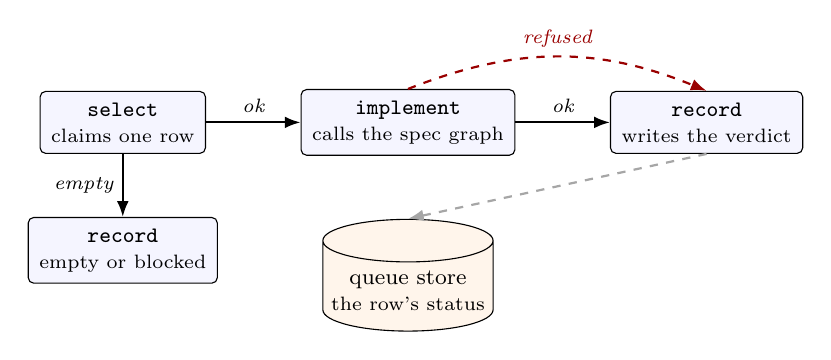
\begin{tikzpicture}[node distance=8mm and 12mm]
  \node[b] (select) {\texttt{select}\\\scriptsize claims one row};
  \node[b, right=of select] (impl) {\texttt{implement}\\\scriptsize calls the spec graph};
  \node[b, right=of impl] (record) {\texttt{record}\\\scriptsize writes the verdict};
  \node[b, below=of select] (none) {\texttt{record}\\\scriptsize empty or blocked};
  \node[s, below=of impl] (store) {queue store\\\scriptsize the row's status};
  \draw[f] (select) -- node[p,above=2pt,midway]{ok} (impl);
  \draw[f] (impl) -- node[p,above=2pt,midway]{ok} (record);
  \draw[f] (select) -- node[p,left=2pt,midway]{empty} (none);
  \draw[bk] (impl.north) to[bend left=22] node[p,above=2pt,midway]{refused} (record.north);
  \draw[sf] (record.south) -- (store.north);
\end{tikzpicture}}
\captionof{figure}{\texttt{queue} claims one row, hands it to the implementer, and records a
verdict. The red edge is the one that took a row from \enquote{stuck Running} to
\enquote{recorded as refused}.}
\end{center}

The three ports of \texttt{select} are the whole reason the queue is readable.
\texttt{ok} means a row was claimed, \texttt{empty} means there was nothing to do, and
\texttt{blocked} means a row exists but something it waits on does not --- and \texttt{blocked}
ends the run on its own edge rather than pretending to have worked. A row that stays
\texttt{Running} after the run ends is the failure this shape exists to prevent: at the
revision this manual describes, a refused callee used to dead-end inside the splice
because the callee's refusal nodes declare no \texttt{ok} port, so no edge fired and the
row was never recorded. The fix wires the refusal by name ---
\texttt{implement.refused}, \texttt{implement.unverified} --- and the queue's own graph now
carries both edges.

The rule for an operator is one sentence: if a row does not leave \texttt{Running}, read
the trace and look at the last node, not at the last message. The verdict is in the
journal even when the record was never written.

\section{Reading a run}

Three commands read a run, and they answer different questions.

\begin{lstlisting}[language=bash]
pii run ls --status suspended         # running|suspended|succeeded|failed
pii run ls --graph queue              # filter by graph name, client-side
pii run get <run_id>                  # the header: graph, status, timing
pii run trace <run_id>                # node by node, with the port that fired
pii run explain <run_id>              # the same journal, summarised
\end{lstlisting}

\texttt{--status} accepts exactly four names and refuses anything else with the list in
the message. \texttt{refused} is a run status the store knows but not one the filter
accepts, which is a small asymmetry worth knowing before you script it.

\texttt{pii run get} distinguishes three answers that look alike in a hurry. A run the
daemon holds but has not journalled yet answers \texttt{accepted} --- the id exists and the
journal has not materialised, so you poll again. A stored state answers
\texttt{running}, \texttt{suspended}, \texttt{succeeded} or \texttt{failed}. An id the
daemon has never heard of answers \enquote{unknown to this daemon}: it was never issued, or
the daemon restarted and lost an accepted-but-never-journalled start. Polling an
\texttt{accepted} id until it becomes terminal is correct; treating the first
\texttt{not found} as a failure is not, and the measured baseline is that a validated start
never polls \texttt{not found} for ever --- a start the run's own validation refuses still
returns an id, then goes to \texttt{failed} with the reason in the trace.

\begin{center}
\resizebox{\linewidth}{!}{
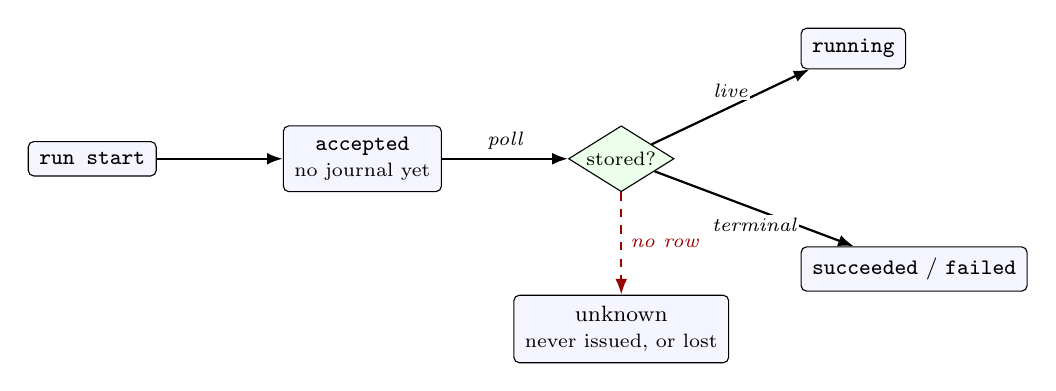
\begin{tikzpicture}[node distance=13mm and 16mm]
  \node[b] (start) {\texttt{run start}};
  \node[b, right=of start] (acc) {\texttt{accepted}\\\scriptsize no journal yet};
  \node[v, right=of acc] (state) {stored?};
  \node[b, right=of state, yshift=14mm] (run) {\texttt{running}};
  \node[b, right=of state, yshift=-14mm] (done) {\texttt{succeeded} / \texttt{failed}};
  \node[b, below=of state] (unknown) {unknown\\\scriptsize never issued, or lost};
  \draw[f] (start) -- (acc);
  \draw[f] (acc) -- node[p,above=2pt,midway]{poll} (state);
  \draw[f] (state) -- node[p,above=2pt,midway]{live} (run);
  \draw[f] (state) -- node[p,below=2pt,midway]{terminal} (done);
  \draw[bk] (state) -- node[p,right=2pt,midway]{no row} (unknown);
\end{tikzpicture}}
\captionof{figure}{Three answers from \texttt{run get}, and only one of them is a polling state.
The red edge is the reading that is a real problem: an id the daemon never issued, or lost
across a restart before its journal was written.}
\end{center}

Read a trace from the end. The last \texttt{NodeFinished} names the node and the port it
took, and that pair is the decision the run made. A run that stopped without reaching a
terminal node has not failed loudly --- it has failed quietly, which is the failure mode
the journal exists to make visible. The events you will read most are
\texttt{Started}, \texttt{TickStarted}, \texttt{NodeStarted}, \texttt{NodeFinished},
\texttt{NodeFailed}, \texttt{NodeProgress}, \texttt{NodeCancelled}, \texttt{NodeDead},
\texttt{NodeInterrupted}, \texttt{Suspended}, \texttt{Resumed} and \texttt{NodeObserved};
Chapter~\ref{ch:what} lists all seventeen.

\texttt{NodeProgress} deserves its own sentence, because it is the only event that
separates a slow node from a wedged one: it carries elapsed milliseconds and the child's CPU
milliseconds, so \emph{elapsed grows, CPU flat} is a node waiting on something that will
never answer, while \emph{both grow} is a node doing work.

\subsection*{The offline trace, and its queries}

When the daemon is down, the same journal is readable from the store file directly, and
the offline form answers more questions than the online one.

\begin{lstlisting}[language=bash]
pii graph trace <run_id> --db ~/.local/state/pii/store.redb
pii graph trace <run_id> --db ... --terminal
pii graph trace <run_id> --db ... --node-status verify
pii graph trace <run_id> --db ... --reason refused
pii graph trace <run_id> --db ... --overlapped code,docs
\end{lstlisting}

With no query at all, the command prints the journal as NDJSON: one event per line, each
with a sequence number.
\texttt{--terminal} prints the run's terminal value, \texttt{--node-status} prints one
node's last port, \texttt{--reason} prints why a refusal node refused,
\texttt{--max-batch-width} reports how wide the scheduler's batches ran, and
\texttt{--overlapped a,b} answers whether two nodes were ever in flight at the same time ---
which is the question you ask when a graph is suspected of hiding a serialisation.

\subsection*{When a run needs a hand}

Four commands exist for runs that will not finish on their own, and they differ in what
they do to the evidence.

\begin{center}
\begin{tabular}{@{}p{0.26\textwidth}p{0.62\textwidth}@{}}
	\toprule
	\textbf{Command} & \textbf{What it does} \\
	\midrule
        \texttt{pii run resume \textless{}id\textgreater{}} & continues a \texttt{Suspended} run
through its resume
	key \\
        \texttt{pii run retry \textless{}id-> --node \textless{}id\textgreater{}} &
re-runs one node of a finished run \\
        \texttt{pii run abandon \textless{}id-> --reason T} & marks the run
abandoned, with the reason
	recorded \\
        \texttt{pii run cancel \textless{}id-> [--kill]} & cancels a live run;
\texttt{--kill} also kills
	the child \\
	\bottomrule
\end{tabular}
\end{center}

Abandon and cancel are the two that change what retention will later do. A run left
\texttt{Running} or \texttt{Suspended} is never swept, however old it is, so a run you
have given up on stays in the store for ever unless you end it deliberately.

\section{Stores, memory and the indices}

Store maintenance is three commands, and two of them need the daemon stopped.
\texttt{pii store stats} prints one line per table with its row count, then the file's
byte size. \texttt{pii store compact} takes redb's exclusive lock, so a running daemon makes
it refuse rather than copy a file mid-write, and it prints the measured size of each file
before and after. \texttt{pii store prune} takes the same lock, runs one retention sweep and
prints \texttt{pruned N rows}.

\texttt{pii store stats} is the command to run weekly. It prints
\texttt{store.redb \textless{}table-> rows=N} for every table and then
\texttt{store.redb bytes=N}, which together are the only honest growth signal --- the file
size alone is not, because redb never shrinks and a store that has been compacted tells you
nothing about how fast it is filling. \texttt{pii store compact} prints
\texttt{compacted \textless{}name-> \textless{}before-> ->
\textless{}after-> bytes} per file, and a store with nothing to
reclaim prints a near-equal pair, which is the truth rather than a failure.

\texttt{pii store prune} runs one retention sweep under the default policy and prints the
count. The defaults are thirty days for finished runs, seven for node-call events and at
most one thousand rows per sweep; the sweep never removes a \texttt{Running} or
\texttt{Suspended} run, and it keeps any row whose creation time is missing. The daemon
also runs one sweep at boot, so a host that restarts nightly trims itself.

Memory has its own command group, and the two that are used daily are search and the
entity graph: \texttt{pii memory search \textless{}q\textgreater{}} with an optional
\texttt{--k} (six results by
default), and \texttt{pii memory put \textless{}text\textgreater{}} with \texttt{--layer} and
\texttt{--kind} for
a document's tier. \texttt{pii memory tiers} says what sits in each tier,
\texttt{pii memory entity list} gives the entities and their counts, and
\texttt{pii memory neighbours} gives one hop around an entity. The rest of the group
(\texttt{learn}, \texttt{consolidate}, \texttt{link}, \texttt{compact}, \texttt{archive},
\texttt{restore}) is maintenance, and each one either refuses or reports when its
precondition is missing rather than doing half the work.

\texttt{pii index code} and \texttt{pii index docs} fill the code and documentation indices
from a tree, and \texttt{pii skill list} answers what the daemon knows how to do. Both are
read-mostly and safe to re-run: an index command re-reads and updates, it does not
duplicate.

\section{A cadence that works}

The commands above are cheap; the discipline is knowing which ones to run on a clock. The
cadence below is the one Chapter~\ref{ch:operate} assumes, written as a table so it can be
checked rather than remembered.

\begin{longtable}{@{}p{0.13\textwidth}p{0.30\textwidth}p{0.45\textwidth}@{}}
	\toprule
	\textbf{When} & \textbf{Command} & \textbf{What you are looking for} \\
	\midrule
	\endhead
	Every session & \texttt{pii health} & exit 0; \texttt{client:} equals the build line \\
	Every session & \texttt{pii run ls --status running} & a run that should have finished \\
	Daily & the log file, last lines & a log that ends on \texttt{daemon.started} means a
	hard death \\
	Weekly & \texttt{pii store stats} & rows and bytes per table, recorded, so the slope
	exists \\
	Weekly & \texttt{pii disk} & an artefact root growing without an owner \\
	Monthly & \texttt{pii store compact} & the tail slack back; nothing more \\
	Monthly & a restore into a scratch directory & a backup nobody restored is a hope \\
	\bottomrule
\end{longtable}

Two of those rows are worth the cost even on a quiet host. A weekly \texttt{store stats}
sample is what turns \enquote{the disk is filling} into a rate, and a monthly restore into a
scratch state directory is what turns a backup into a backup --- both drills are described
in Chapter~\ref{ch:operate}.

\section{What a quiet day looks like}

A host with nothing to do is not silent, and knowing the small noises saves a false alarm.
The daemon writes a \texttt{daemon.started} event, keeps its health record current, and
runs one retention sweep at boot. If a channel is configured it polls on its interval; if a
worker is configured it says hello once. Nothing else should appear in the log.

The four readings that answer \enquote{is this host doing anything} are
\texttt{pii health} (first three lines: build, client, config hash), \texttt{pii run ls}
(usually an empty list on a host with no work), \texttt{pii cron ls} (the schedules the
daemon knows) and the last three lines of \texttt{\$STATE\_DIR/pii.log}. On a healthy host
the log's last line is a \texttt{daemon.started} only after a restart --- a log that ends on
\texttt{daemon.started} while the process has been up for days means the daemon died hard
and was restarted by the unit, and \texttt{since\_deploy.hard\_deaths} in \texttt{pii
health} will say how many times.

If \texttt{pii run ls} is empty and you expected rows, the question is not \enquote{where did
the runs go} but \enquote{which store is this daemon writing} --- and \texttt{pii health}
answers it with a path. That single habit, reading the store path before believing an empty
list, resolves more \enquote{lost work} reports than any other diagnostic in this manual.

\chapter{Operating}

\label{ch:operate}

This is the chapter nobody reads until something has gone wrong, and it is written for that
moment: short procedures, the exact command for each, the reading that tells you whether
it worked, and the failure modes that have actually happened on this product rather than
the ones a design review imagined. The order is the order of the questions an operator
asks --- can I get the data back, what is the store doing to the disk, what changed when I
upgraded, where is the evidence, and why is the daemon not answering.

\section{Backup and restore}

A backup is offline by construction. \texttt{pii backup} opens each store with redb's
exclusive lock and copies the file while holding that lock, so a running daemon makes the
backup \emph{refuse} --- with the path and the words \enquote{stop the daemon first} ---
instead of copying a file with a writer mid-commit. Each copy is then re-opened as a redb
database and hashed, so a torn or truncated copy is an error rather than a silent bad
backup.

\begin{lstlisting}[language=bash]
systemctl --user stop pii
pii backup /backups/pii-$(date +%F) --dir ~/.local/state/pii
systemctl --user start pii
\end{lstlisting}

The command prints one line per file, with these field names and no others:
\texttt{backed up store.redb (\textless{}bytes-> bytes,
format\_version=\textless{}n->, blake3=\textless{}hash\textgreater{})}.
The same facts go into \texttt{MANIFEST.json} inside the destination, and the manifest is
what a restore checks against. The destination must be new or empty.

\begin{center}
\resizebox{\linewidth}{!}{
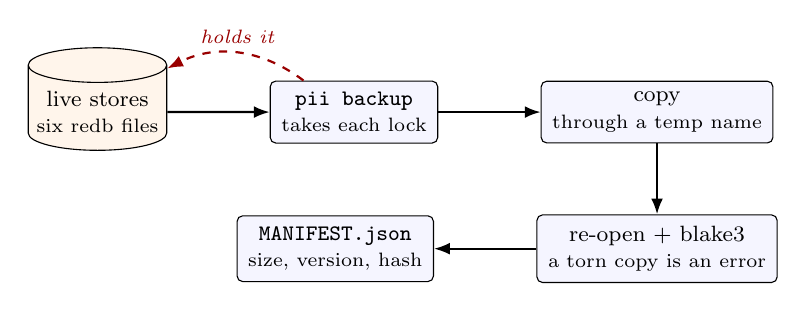
\begin{tikzpicture}[node distance=9mm and 13mm]
  \node[s] (live) {live stores\\\scriptsize six redb files};
  \node[b, right=of live] (lock) {\texttt{pii backup}\\\scriptsize takes each lock};
  \node[b, right=of lock] (copy) {copy\\\scriptsize through a temp name};
  \node[b, below=of copy] (hash) {re-open + blake3\\\scriptsize a torn copy is an error};
  \node[b, left=of hash] (manifest) {\texttt{MANIFEST.json}\\\scriptsize size, version, hash};
  \draw[f] (live) -- (lock);
  \draw[f] (lock) -- (copy);
  \draw[f] (copy) -- (hash);
  \draw[f] (hash) -- (manifest);
  \draw[bk] (lock) to[bend right=32] node[p,above=2pt,midway]{holds it} (live);
\end{tikzpicture}}
\captionof{figure}{A backup that cannot tear. The red edge is the normal case on a live host:
the open fails, the command refuses, and no file is written.}
\end{center}

Two details decide whether the backup is worth having.

First, the backup set is six files: \texttt{store.redb}, \texttt{memory.redb},
\texttt{approval.redb}, \texttt{heal.redb}, \texttt{channel.redb} and
\texttt{timer.redb}. \texttt{pii health} reports seven stores, and the seventh ---
\texttt{queue.redb}, where the work rows live --- is not in the backup set at this
revision. If you rely on the queue, copy that file with the daemon stopped as well, or
record the rows somewhere you can rebuild them from.

Second, \texttt{--dir} names the directory that holds the stores, and the durable pair
(channel, timer) defaults to \texttt{\textless{}state dir\textgreater{}/durable}, not to the
directory beside the
main store. A backup run with \texttt{--dir \textless{}state dir\textgreater{}} therefore
captures the main store,
memory, approvals and heal, and reports nothing for channel and timer because those files
are one level down. Run a second backup with \texttt{--dir \textless{}state
dir\textgreater{}/durable} if cursors
and timers matter to you --- and they matter the first time a channel replays from the
start after a restore.

Restore verifies every file's hash against the manifest before touching the target, never
deletes, and refuses a store that is in use.

\begin{lstlisting}[language=bash]
systemctl --user stop pii
pii restore /backups/pii-2026-11-04 --dir ~/.local/state/pii           # refuses if a target exists
pii restore /backups/pii-2026-11-04 --dir ~/.local/state/pii --force   # moves the old store aside
systemctl --user start pii
\end{lstlisting}

\texttt{--force} does not delete: it moves the existing store to
\texttt{\textless{}name\textgreater{}.redb.old-\textless{}ms\textgreater{}} and leaves the
decision about the old file to you. That is
deliberate --- the one file you are most likely to want after a bad restore is the store
the restore replaced.

\section{Retention}

Retention is the only code in the product that deletes run data, so its rules are worth
knowing before you need them. The policy has three numbers and three guards.

\begin{center}
\begin{tabular}{@{}p{0.26\textwidth}p{0.62\textwidth}@{}}
	\toprule
	\textbf{Setting} & \textbf{Default and meaning} \\
	\midrule
	run age & 30 days: a finished run's header, journal and snapshots go past this age \\
	node-event age & 7 days: a finished run's node-call events go past this age \\
	rows per sweep & 1\,000: the sweep's whole budget, so a first run on a large store
	cannot hold a write transaction for minutes \\
	\bottomrule
\end{tabular}
\end{center}

The guards are the part that matters:

\begin{enumerate}
	\item A run whose status is \texttt{Running} or \texttt{Suspended} is never removed,
	however old it is, because the daemon may still resume it.
	\item A row that cannot be dated is kept. A run created before the clock was recorded
	carries \texttt{created\_ms} of zero, and deleting on a missing timestamp would destroy
	exactly the runs an operator is looking for.
	\item The sweep is bounded per call, so it is a trim rather than a migration.
\end{enumerate}

One sweep runs when the daemon starts, and \texttt{pii store prune} runs one on demand. The
command prints \texttt{pruned N rows} and exits 0; the store also records a
\texttt{store.retention.swept} event carrying the count, but only when something was
removed. A sweep that removes nothing is silent, which is why the count on stdout is the
number to read.

\section{What retention actually removes}

The three rules have an order of precedence, and the order is not the one people assume.
Age selects candidates; a live run is excluded; an undatable row is excluded; then the
per-sweep budget truncates whatever remains.

\begin{center}
\resizebox{\linewidth}{!}{
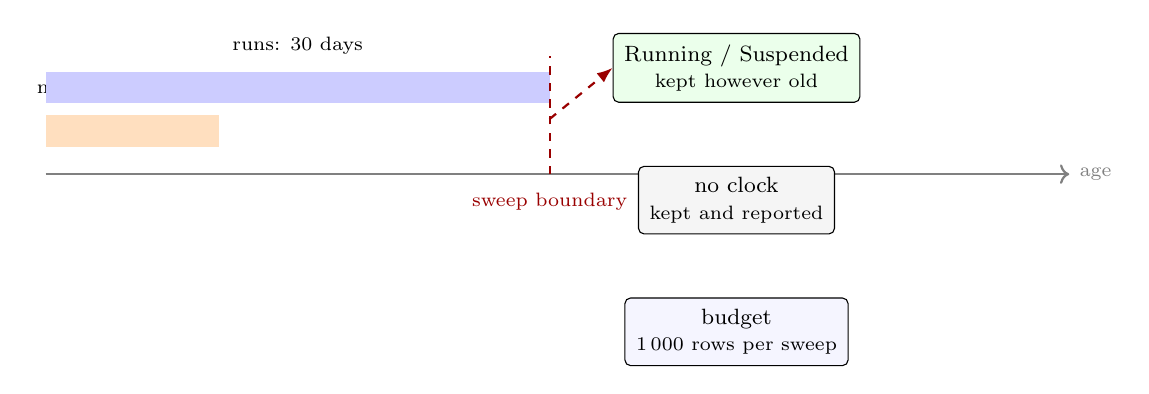
\begin{tikzpicture}[node distance=8mm and 12mm]
  \draw[->, thick, gray] (0,0) -- (13,0) node[right, font=\scriptsize] {age};
  \fill[orange!25] (0,0.35) rectangle (2.2,0.75);
  \node[font=\scriptsize, above=2pt] at (1.1,0.78) {node events: 7 days};
  \fill[blue!20] (0,0.9) rectangle (6.4,1.3);
  \node[font=\scriptsize, above=2pt] at (3.2,1.33) {runs: 30 days};
  \draw[dashed, red!60!black, thick] (6.4,0) -- (6.4,1.5);
  \node[font=\scriptsize, red!60!black, below=2pt] at (6.4,-0.05) {sweep boundary};
  \node[b, fill=green!8, anchor=west] (live) at (7.2,1.35)
    {Running / Suspended\\\scriptsize kept however old};
  \node[b, fill=gray!8, below=of live] (undated) {no clock\\\scriptsize kept and reported};
  \node[b, below=of undated] (budget) {budget\\\scriptsize 1\,000 rows per sweep};
  \draw[bk] (6.4,0.7) -- (live.west);
\end{tikzpicture}}
\captionof{figure}{Three rules, in order of precedence: age bounds the sweep, a live run is
never swept, and a row that cannot be dated is kept. The budget is last, so a large store trims
over several sweeps rather than one long transaction.}
\end{center}

A run that will never finish is therefore never collected. If you see one, park or cancel
it deliberately --- \texttt{pii run abandon} with a reason, or \texttt{pii run cancel} ---
and retention will collect it thirty days after it ended. Retention will not make that
decision for you, and should not: the difference between trimming and losing work in flight
is this guard.

\section{Compaction is not retention}

These two get confused, and the confusion costs a maintenance window that reclaims nothing.
Compaction reclaims free pages \emph{inside} a file; retention removes rows. redb never
returns space to the filesystem except at the end of the file, and only compaction moves
that boundary.

The measured pairs from this product's own runbook are the honest expectation:

\begin{center}
\begin{tabular}{@{}p{0.50\textwidth}p{0.38\textwidth}@{}}
	\toprule
	\textbf{Store state} & \textbf{Before $\rightarrow$ after} \\
	\midrule
	fragmented: 20 sessions of 400\,KB, every other one deleted &
	13\,111\,296 $\rightarrow$ 6\,623\,232 bytes \\
	a store after 400 runs through a daemon & 1\,048\,576 $\rightarrow$ 786\,432 bytes \\
	idle auxiliary stores (memory, approval, heal, channel, timer) &
	1\,056\,768 $\rightarrow$ 36\,864 bytes each \\
	\bottomrule
\end{tabular}
\end{center}

So on a store that has only grown with runs, expect the tail slack back and nothing more.
The 400-run row is the one to remember: it is a two-hundred-kilobyte improvement on a
megabyte file, which is not a reason to schedule an outage. The auxiliary row is the reason
to run compaction at all --- five stores that were preallocated and never wrote shrank by
about 97\,\%.

\section{The restore drill}

A backup nobody has restored is a hope. The drill is short, it uses a scratch state
directory, and it is the only way to know that the manifest, the hashes and the binary's
format version all agree.

\begin{center}
\resizebox{\linewidth}{!}{
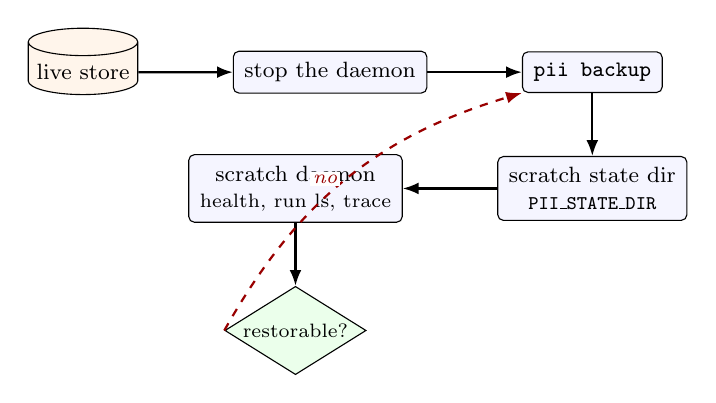
\begin{tikzpicture}[node distance=8mm and 12mm]
  \node[s] (store) {live store};
  \node[b, right=of store] (stop) {stop the daemon};
  \node[b, right=of stop] (copy) {\texttt{pii backup}};
  \node[b, below=of copy] (scratch) {scratch state dir\\\scriptsize \texttt{PII\_STATE\_DIR}};
  \node[b, left=of scratch] (probe) {scratch daemon\\\scriptsize health, run ls, trace};
  \node[v, below=of probe] (verdict) {restorable?};
  \draw[f] (store) -- (stop);
  \draw[f] (stop) -- (copy);
  \draw[f] (copy) -- (scratch);
  \draw[f] (scratch) -- (probe);
  \draw[f] (probe) -- (verdict);
  \draw[bk] (verdict.west) to[bend left=22] node[p,left=2pt,midway]{no} (copy.south west);
\end{tikzpicture}}
\captionof{figure}{A backup is a backup once it has been restored into a scratch state directory
and read there. Restoring over the live store destroys the evidence you would need if the
restore is wrong.}
\end{center}

\begin{lstlisting}[language=bash]
mkdir -p /projects/_tmp/restore-drill
pii restore /backups/pii-2026-11-04 --dir /projects/_tmp/restore-drill
PII_STATE_DIR=/projects/_tmp/restore-drill pii store stats
PII_STATE_DIR=/projects/_tmp/restore-drill pii graph trace <run_id> \
  --db /projects/_tmp/restore-drill/store.redb --terminal
\end{lstlisting}

Three readings close the drill. \texttt{store stats} prints a row count per table, so an
empty journal is visible immediately. A trace on a known run id prints that run's terminal
value, which proves the journal survived the round trip. And a daemon started on the
scratch directory with a different runtime dir proves the binary can open the restored
format version --- the one thing a restore cannot repair is a store written by a newer
build.

\section{Upgrading}

An upgrade is four steps and one expected non-zero exit code. The exit code is the part
that alarms people: immediately after installing a new binary and before restarting the
service, \texttt{pii health} exits 3 and prints a \texttt{DRIFT} line, because the client
is the new build and the daemon is still the old process. That is the instrument working.
It returns 0 only after the restart.

\begin{lstlisting}[language=bash]
systemctl --user stop pii
pii backup /backups/pii-pre-upgrade --dir ~/.local/state/pii
bash deploy/install-pii.sh                                      # card-gated, moves the old aside
pii health                                                      # expect 3 + DRIFT
systemctl --user restart pii
pii health && pii --version                                     # expect 0, same revision
\end{lstlisting}

\begin{center}
\resizebox{\linewidth}{!}{
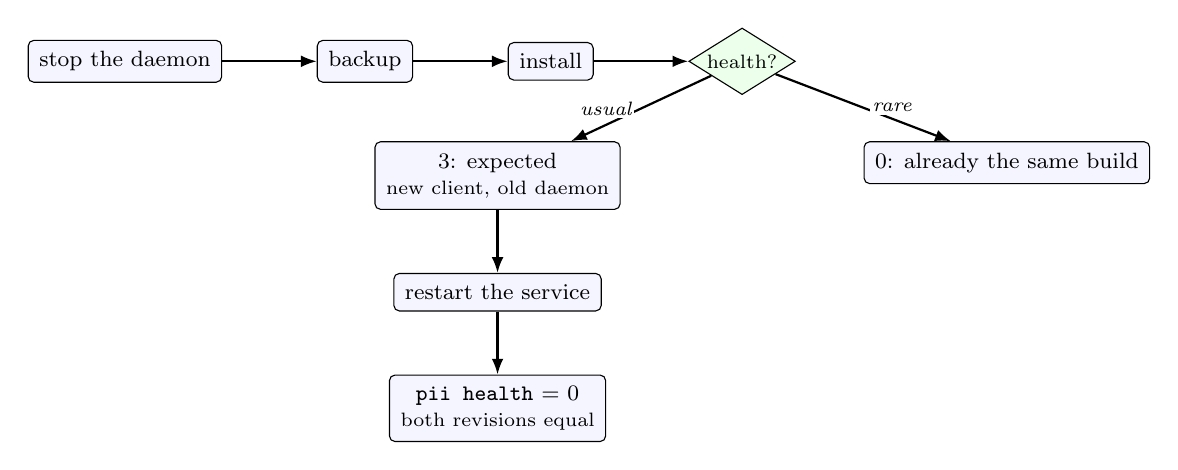
\begin{tikzpicture}[node distance=8mm and 12mm]
  \node[b] (stop) {stop the daemon};
  \node[b, right=of stop] (backup) {backup};
  \node[b, right=of backup] (install) {install};
  \node[v, right=of install] (drift) {health?};
  \node[b, below left=of drift] (three) {3: expected\\\scriptsize new client, old daemon};
  \node[b, below right=of drift] (zero) {0: already the same build};
  \node[b, below=of three] (restart) {restart the service};
  \node[b, below=of restart] (verify) {\texttt{pii health} = 0\\\scriptsize both revisions equal};
  \draw[f] (stop) -- (backup);
  \draw[f] (backup) -- (install);
  \draw[f] (install) -- (drift);
  \draw[f] (drift) -- node[p,left=2pt,midway]{usual} (three);
  \draw[f] (drift) -- node[p,right=2pt,midway]{rare} (zero);
  \draw[f] (three) -- (restart);
  \draw[f] (restart) -- (verify);
\end{tikzpicture}}
\captionof{figure}{The upgrade sequence, with the reading that is correct and looks wrong. A
\texttt{3} here is not a failed upgrade; it is the proof that the install replaced the binary
and the service has not yet been restarted.}
\end{center}

The state directory is forward-compatible only in one direction. Every store carries a
format version stamped on create or first open, and a binary that meets a newer version
refuses to open it:

\begin{lstlisting}[language=bash]
error: invalid: store '/var/lib/pii/memory.redb' has format version 99, which is newer
than the version 1 this binary understands; upgrade pii or use a different store path
\end{lstlisting}

The daemon exits 2 and writes nothing to the file. The remedy is a binary that understands
that version, or a restore of a backup taken by the older build --- never an edit of the
stamp.

Rollback is the install script's inverse and it moves rather than copies:
\texttt{bash deploy/rollback-pii.sh} stops the unit, restores the newest
\texttt{\$PREFIX.old-\textless{}epoch\textgreater{}} contents, keeps what it replaced under
\texttt{\$PREFIX.rolledback-\textless{}epoch\textgreater{}}, and prints each file. Then
\texttt{daemon-reload} and \texttt{restart}, then \texttt{pii health} for a 0.

\subsection*{The gate the card quotes}

No install runs without a deploy card for the revision being installed. The card is a JSON
file with five required fields --- \texttt{incident} (id, fingerprint, count),
\texttt{change} (branch, revision, diff stat), \texttt{proof} (red on base, green on
branch), \texttt{gate} (verdict) and \texttt{rollback} (rehearsal) --- and a card missing
any of them is refused with the field named and no approval path printed. Approval is bound
to the revision the card names, and every decision appends one line to the operator record
(\texttt{PII\_ACTS}, default \texttt{\_tmp/autonomy/operator-acts.log}).

The gate verdict has a condition attached that is easy to miss: a deploy run must quote a
\emph{fresh-tree} gate, and a \texttt{mode=routine} verdict is not release evidence. A
routine gate runs in the working tree against a warm target; a fresh gate exports
\texttt{HEAD} and builds in a throwaway directory. When the two disagree, believe the fresh
one --- a gate can be green in a tree and red in a clean clone.

\section{Logs, audit, and the death that leaves no line}

The daemon writes events as JSON lines, one per event, each stamped with \texttt{ts\_ms}.
The log is off unless a path is set. Three keys control it, and each has a flag that
overrides it.

\begin{longtable}{@{}p{0.24\textwidth}p{0.30\textwidth}p{0.38\textwidth}@{}}
	\toprule
	\textbf{Key} & \textbf{Default} & \textbf{Flag} \\
	\midrule
	\endhead
	\texttt{[core].log\_file} & absent: no log file & \texttt{--log-file} \\
	\texttt{[core].log\_rotate\_bytes} & 10\,485\,760 (10 MiB); 0 never rotates &
	\texttt{--log-rotate-bytes} \\
	\texttt{[core].log\_keep\_files} & 5 rotated files besides the live one &
	\texttt{--log-keep-files} \\
	\bottomrule
\end{longtable}

Rotation renames rather than truncates: \texttt{pii.log} becomes \texttt{pii.log.1},
\texttt{pii.log.1} becomes \texttt{pii.log.2}, and the oldest is discarded, so disk use is
bounded by about \texttt{(keep + 1) * rotate\_bytes}. The file is rotated \emph{before} a
line would push it past the limit, so a single pathological line can exceed the bound once.

Denials are separate and always on: they go to \texttt{audit.log} in the store directory,
rotated the same way, whatever the log file is set to. If you are investigating a
permission problem and the daemon log is clean, read \texttt{audit.log}.

The one reading that matters is the last line. A log that ends on \texttt{daemon.started}
with no \texttt{daemon.stopped} means the process died hard --- a \texttt{kill -9}, an OOM
kill, a machine reset. \texttt{pii health} agrees: \texttt{since\_deploy.starts} and
\texttt{since\_deploy.hard\_deaths} are counters kept across restarts, so a host that has
restarted eleven times and died hard twice says so in two lines.

\section{Disk is owned, bounded and visible}

Disk needed its own command because the obvious answers are about the wrong filesystem. The
measured incident: the container's \texttt{/} is a 288\,GB overlay that reached 16\,GB
free (95\,\%), while \texttt{/projects} --- a separate 594\,GB volume --- had 147\,GB free.
The gate refuses to run below a 12\,GB floor on \texttt{/}, so work stopped, and
\texttt{cargo clean} on the repository freed 152\,GB on the volume that was never short.

\begin{center}
\resizebox{\linewidth}{!}{
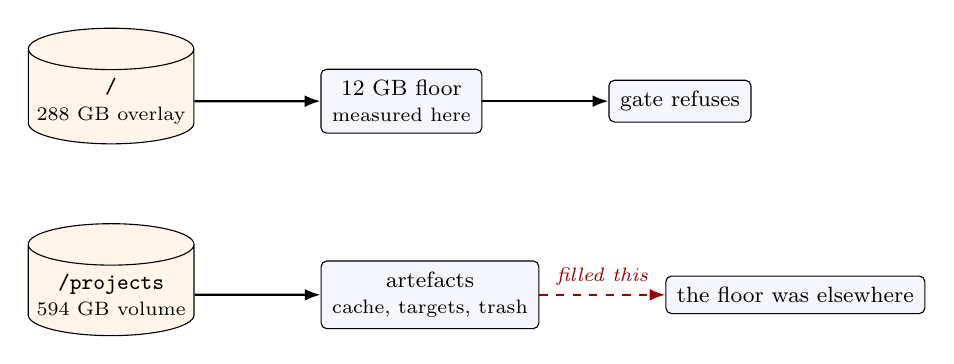
\begin{tikzpicture}[node distance=10mm and 16mm]
  \node[s] (overlay) {\texttt{/}\\\scriptsize 288 GB overlay};
  \node[b, right=of overlay] (floor) {12 GB floor\\\scriptsize measured here};
  \node[b, right=of floor] (refuse) {gate refuses};
  \node[s, below=of overlay] (vol) {\texttt{/projects}\\\scriptsize 594 GB volume};
  \node[b, right=of vol] (artefacts) {artefacts\\\scriptsize cache, targets, trash};
  \node[b, right=of artefacts] (lie) {the floor was elsewhere};
  \draw[f] (overlay) -- (floor);
  \draw[f] (vol) -- (artefacts);
  \draw[f] (floor) -- (refuse);
  \draw[bk] (artefacts) -- node[p,above=2pt,midway]{filled this} (lie);
\end{tikzpicture}}
\captionof{figure}{The mismatch that hid the growth: the floor was measured on \texttt{/}, the
artefacts landed on \texttt{/projects}. Freeing the volume looked like progress and was worth
nothing.}
\end{center}

\texttt{pii disk} prints the artefact table and \emph{both} free-space lines, which is the
whole fix for that class of confusion. Four mechanism families fill the disk, and each has
an owner now:

\begin{center}
\begin{tabular}{@{}p{0.30\textwidth}p{0.62\textwidth}@{}}
	\toprule
	\textbf{Mechanism} & \textbf{Owner and bound} \\
	\midrule
	the warm gate cache & ceiling of 40\,GiB
	(\texttt{FRESH\_GATE\_CACHE\_MAX\_GB}); trimmed before a build, never while a build is
	live. It once reached 105.8\,GiB because nothing bounded it. \\
        one-off experiment targets & \texttt{\_tmp/targets/\textless{}purpose\textgreater{}}
with a TTL of 7 days
	(\texttt{DISK\_TTL\_DAYS}), removed by \texttt{cargo xtask disk --gc} \\
	trash & dated directories with a retention window, not a build artefact \\
	failed gate exports & removed after \texttt{DISK\_EXPORT\_TTL\_HOURS} unless a gate
	still owns one \\
	\bottomrule
\end{tabular}
\end{center}

\texttt{cargo xtask disk --gc} refuses to remove anything while a cargo or rustc is live
and prints why, which is the guard that keeps the cleanup from becoming the incident. The
12\,GB floor is not lowered to make a gate pass; if the floor is what stops you, the answer
is space.

\section{When the daemon is wedged}

The sequence is short and it is ordered so that no step destroys evidence the next one
needs.

\begin{enumerate}
	\item \texttt{pii health --json} with a short timeout. No answer within a few seconds
	means the daemon is wedged or dead, and exit 2 means nothing is listening at all.
	\item Read the last lines of the log file before stopping anything. A
	\texttt{daemon.started} with no \texttt{daemon.stopped} is a hard death; the last
	non-start event names what it was doing.
	\item \texttt{systemctl --user stop pii}. Shutdown waits at most five seconds for
	in-flight blocking work, then abandons it and exits anyway. If something was stuck,
	stderr carries exactly one line:
	\enquote{pii: shutdown drain exceeded 5s; abandoning in-flight blocking work}. That
	line is stderr only --- it is in the journal, not in the log file.
	\item If systemd had to SIGKILL it, nothing is lost structurally: the store is a
	transactional redb file, and the daemon reconciles interrupted runs on boot. Start it
	and read \texttt{pii health}.
	\item A run that was mid-flight comes back as \texttt{Running} or \texttt{Failed}, with
	a \texttt{NodeInterrupted} event in its journal for the node that was left in flight.
	Read the trace before resuming it.
\end{enumerate}

\section{Failure modes that have actually happened}

\begin{longtable}{@{}p{0.28\textwidth}p{0.64\textwidth}@{}}
	\toprule
	\textbf{Symptom} & \textbf{Cause and what to check} \\
	\midrule
	\endhead
	Every graph run fails in a second, with no output &
	A model id the provider does not serve. The old id had not existed for months and the
	graph died at spawn; run \texttt{pii graph lint} and read the model in the graph. \\
	The daemon answers, but the store is empty & Two different \texttt{PII\_STATE\_DIR}
	values --- one for the daemon, another for your shell --- or a daemon whose
	\texttt{--store} points at the runtime directory. Read the path in \texttt{pii health}. \\
	A row stays \texttt{Running} for ever & A callee refused and no edge carried the
	refusal. At this revision the queue wires \texttt{refused} and \texttt{unverified} by
	name; an older graph dead-ends inside the splice. Trace the run; the refusal is in the
	journal. \\
	The coder stops and says no write tool is available & The graph's \texttt{caps} omit
	\texttt{fs\_write}, so the node may not hold it. That is the capability ladder working,
	not a bug. \\
	The gate refuses with a disk message on a full disk & The floor now names the filesystem
	it measured. A message that names only \texttt{/} while the artefacts land elsewhere is
	an older binary. \\
	\texttt{backup} refuses with \enquote{cannot be opened exclusively} & The daemon is
	running and holds the lock. Stop it; the refusal is the no-tear guarantee, not a fault. \\
	\texttt{health} prints \texttt{UNVERIFIED: daemon build revision is unknown} & The
	running binary was built without its revision --- an export build that did not receive
	\texttt{PII\_BUILD\_REVISION}. Rebuild with the installer. \\
	A channel replays its backlog after a restore & The channel cursor lives in
	\texttt{durable/channel.redb}, and a backup of the store directory does not include it.
	Back that directory up too. \\
	\bottomrule
\end{longtable}

\section{The first five minutes of an incident}

Order matters more than completeness. Five checks establish whether you are looking at a
process problem, a data problem or an environment problem, and each takes seconds.

\begin{longtable}{@{}p{0.06\textwidth}p{0.30\textwidth}p{0.56\textwidth}@{}}
	\toprule
	\textbf{Step} & \textbf{Command} & \textbf{What it settles} \\
	\midrule
	\endhead
	1 & \texttt{pii health} & Is anything answering, and is it this build? Exit 2 is a
	process problem; exit 3 is a deployment problem. \\
	2 & \texttt{pii run ls --status running} & Is work in flight? A run that should have
	finished is a graph problem, not a daemon problem. \\
	3 & \texttt{pii disk} & Is the host out of space on the filesystem the artefacts use?
	A gate or a write failing at 95\,\% looks like a code defect. \\
	4 & the log's last ten lines & Did it die hard, and what was the last thing it did? \\
	5 & \texttt{pii store stats} & Is the store growing at a rate that explains the
	symptom, and does the row count match what you expect? \\
	\bottomrule
\end{longtable}

The order is not arbitrary. Checking the store before the disk gives you a row count you
cannot interpret; checking runs before health gives you a list from a daemon that may not
be the binary you think. Health first, because every later reading depends on knowing which
process produced it.

\section{Two rules that keep a host boring}

The rest of this manual is detail; these two rules prevent most of the incidents in it.

\textbf{Never point a second process at a live state directory.} The stores are exclusive,
the daemon claims the durable pair before it binds, and a second daemon will be refused ---
but a CLI command with a different \texttt{PII\_STATE\_DIR} will not be refused, it will
quietly read a different store and report an empty world. If a reading surprises you, the
first question is which store it came from.

\textbf{Never delete what you can move.} The installer moves old binaries aside, the
restore moves the replaced store aside, retention keeps undatable rows, and compaction
refuses while a writer holds the file. Every one of those behaviours exists because the
alternative destroyed something nobody could reconstruct. When a procedure in this chapter
seems to be missing a cleanup step, that is the step it is missing on purpose.

\chapter{Command reference}

\label{ch:commands}

This chapter is the complete surface of the \texttt{pii} binary: every group the dispatcher
accepts, the verbs inside each group, the flags each verb reads, and --- the part that is
usually missing from a command reference --- what the verb does to the stores on disk. A
flag is easy to look up; the difference between a command that asks the daemon to write and
one that opens the same file behind the daemon's back is what corrupts an installation.

Every group below was read from \texttt{crates/pii-cli/src/} and matched against the captured
help output. Where a group has no help text of its own (several have none), the flags were
read from the parser, which is the authority.

\section{The shape of the surface}

The first argument selects a group; everything after it belongs to the group. An unknown
first argument prints the usage string and exits 2. There is no plugin mechanism and no
argument-file syntax: what the binary accepts is what this chapter lists.

\begin{center}
\begin{minipage}{\linewidth}
\centering
\resizebox{\linewidth}{!}{%
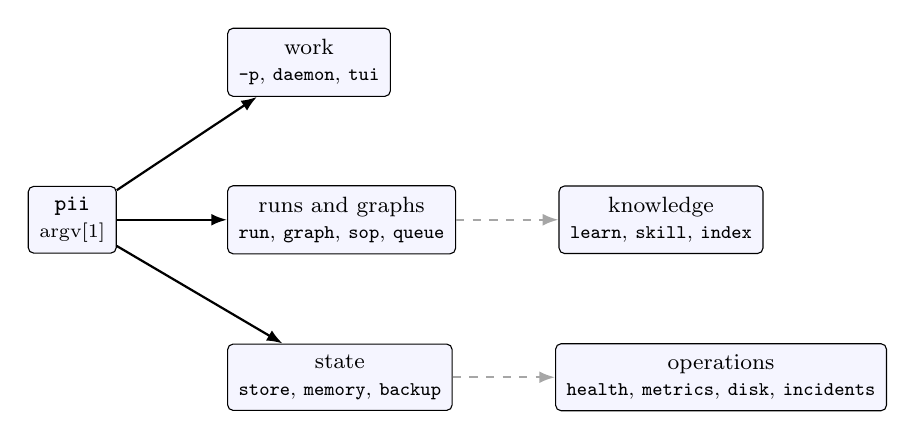
\begin{tikzpicture}[node distance=12mm and 14mm]
  \node[b] (cli) {\texttt{pii}\\\scriptsize argv[1]};
  \node[b, right=14mm of cli, yshift=20mm] (work) {work\\\scriptsize \texttt{-p}, \texttt{daemon}, \texttt{tui}};
  \node[b, right=14mm of cli] (run) {runs and graphs\\\scriptsize \texttt{run}, \texttt{graph}, \texttt{sop}, \texttt{queue}};
  \node[b, right=14mm of cli, yshift=-20mm] (state) {state\\\scriptsize \texttt{store}, \texttt{memory}, \texttt{backup}};
  \node[b, right=13mm of run] (know) {knowledge\\\scriptsize \texttt{learn}, \texttt{skill}, \texttt{index}};
  \node[b, right=13mm of state] (ops) {operations\\\scriptsize \texttt{health}, \texttt{metrics}, \texttt{disk}, \texttt{incidents}};
  \draw[f] (cli) -- (work);
  \draw[f] (cli) -- (run);
  \draw[f] (cli) -- (state);
  \draw[sf] (run) -- (know);
  \draw[sf] (state) -- (ops);
\end{tikzpicture}}
\captionof{figure}{Thirty-three groups plus \texttt{-{}-version}. The grouping is by what the operator is doing, not by which crate implements the verb.}
\end{minipage}
\end{center}

Three paths to state exist, and a command takes exactly one of them.

\begin{center}
\begin{minipage}{\linewidth}
\centering
\resizebox{\linewidth}{!}{%
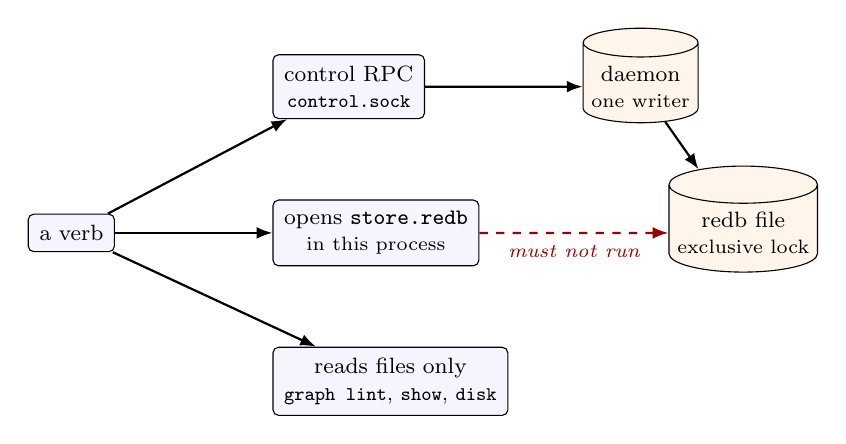
\begin{tikzpicture}[node distance=12mm and 18mm]
  \node[b] (cmd) {a verb};
  \node[b, above right=12mm and 20mm of cmd] (rpc) {control RPC\\\scriptsize \texttt{control.sock}};
  \node[b, right=20mm of cmd] (open) {opens \texttt{store.redb}\\\scriptsize in this process};
  \node[b, below right=12mm and 20mm of cmd] (file) {reads files only\\\scriptsize \texttt{graph lint}, \texttt{show}, \texttt{disk}};
  \node[s, right=20mm of rpc] (daemon) {daemon\\\scriptsize one writer};
  \node[s, right=24mm of open] (store) {redb file\\\scriptsize exclusive lock};
  \draw[f] (cmd) -- (rpc);
  \draw[f] (cmd) -- (open);
  \draw[f] (cmd) -- (file);
  \draw[f] (rpc) -- (daemon);
  \draw[f] (daemon) -- (store);
  \draw[bk] (open) -- node[p, below=3pt, midway]{must not run} (store);
\end{tikzpicture}}
\captionof{figure}{The rule behind every \enquote{daemon must be stopped} message: redb takes an exclusive lock, so a verb that opens the store directly and a daemon that already holds it cannot both proceed.}
\end{minipage}
\end{center}

\begin{longtable}{@{}>{\raggedright\arraybackslash}p{0.20\textwidth}>{\raggedright\arraybackslash}p{0.44\textwidth}>{\raggedright\arraybackslash}p{0.26\textwidth}@{}}
  \toprule
  \textbf{Group} & \textbf{Verbs} & \textbf{Path to state} \\
  \midrule
  \endhead
  \texttt{-{}-version} & none & none \\
  \texttt{-p} & one prompt, options & daemon if up, else in-process \\
  \texttt{daemon} & foreground server & owns the stores \\
  \texttt{graph} & \texttt{lint}, \texttt{check}, \texttt{show}, \texttt{run}, \texttt{resume}, \texttt{trace}, \texttt{list}, \texttt{explain}, \texttt{edit} & files, or \texttt{--db} directly \\
  \texttt{sop} & \texttt{compile}, \texttt{lint}, \texttt{show}, \texttt{run}, \texttt{resume} & \texttt{--db} directly \\
  \texttt{run} & \texttt{ls}, \texttt{start}, \texttt{get}, \texttt{trace}, \texttt{explain}, \texttt{resume}, \texttt{retry}, \texttt{abandon}, \texttt{cancel} & RPC \\
  \texttt{queue} & \texttt{add}, \texttt{ls}, \texttt{claim} & RPC \\
  \texttt{store} & \texttt{compact}, \texttt{stats}, \texttt{prune} & \texttt{store.redb} directly \\
  \texttt{backup}, \texttt{restore} & one positional each & copies the store files \\
  \texttt{memory} & \texttt{search}, \texttt{put}, \texttt{learn}, \texttt{consolidate}, \texttt{entity}, \texttt{link}, \texttt{neighbours}, \texttt{compact}, \texttt{show}, \texttt{tiers}, \texttt{archive}, \texttt{restore} & RPC, or \texttt{memory.redb} \\
  \texttt{approve} & \texttt{ls}, \texttt{allow}, \texttt{deny} & RPC \\
  \texttt{heal} & \texttt{ls}, \texttt{show} & RPC \\
  \texttt{cron}, \texttt{net}, \texttt{worker}, \texttt{sys} & \texttt{ls}; \texttt{status}, \texttt{reload} & RPC \\
  \texttt{health} & none, \texttt{-{}-json} & RPC \\
  \texttt{metrics} & none & RPC \\
  \texttt{disk} & none, \texttt{-{}-root} & filesystem only \\
  \texttt{incidents} & \texttt{scan}, \texttt{show}, \texttt{distance} & files, or a store dir \\
  \texttt{loop} & \texttt{emit}, \texttt{events} & one NDJSON file \\
  \texttt{deploy-card} & \texttt{render}, \texttt{approve}, \texttt{refuse} & card file and an acts log \\
  \texttt{learn} & \texttt{scan}, \texttt{list}, \texttt{show}, \texttt{verify}, \texttt{promote}, \texttt{promotions}, \texttt{revert}, \texttt{ledger} & \texttt{store.redb} \\
  \texttt{skill} & \texttt{add}, \texttt{list}, \texttt{show}, \texttt{explain}, \texttt{edit} & RPC, or \texttt{memory.redb} \\
  \texttt{index} & \texttt{code}, \texttt{docs} & RPC \\
  \texttt{mqtt} & \texttt{ls}, \texttt{sub}, \texttt{pub}, \texttt{send} & broker, not the store \\
  \texttt{treat} & \texttt{export}, \texttt{import}, \texttt{apply}, \texttt{list} & healer store and files \\
  \texttt{lane} & \texttt{plan}, \texttt{run}, \texttt{rev} & writes a plan, starts nothing in \texttt{plan} \\
  \texttt{soak} & none, flags only & RPC against a socket \\
  \texttt{tui} & none & loopback or socket \\
  \texttt{sandbox-exec}, \texttt{worker-exec} & \texttt{argv}, frames & process only \\
  \texttt{project} & \texttt{init} & writes a scaffold \\
  \bottomrule
\end{longtable}

\section{Starting work}

\subsection*{\texttt{pii -{}-version}}

One line, the version compiled into the binary. It is the only group that touches nothing.

\subsection*{\texttt{pii -p "<prompt>"}}

The headless entry point. It prefers a live daemon socket; without one it builds the engine
in this process and serves the same connection over a loopback duplex. It never starts a
daemon. When stdout is not a terminal, JSON is the default output format.

\begin{center}
\begin{tabular}{@{}>{\raggedright\arraybackslash}p{0.22\textwidth}>{\raggedright\arraybackslash}p{0.68\textwidth}@{}}
  \toprule
  \textbf{Flag} & \textbf{Effect} \\
  \midrule
  \texttt{-{}-json} & machine-readable result; the default when stdout is not a TTY \\
  \texttt{-{}-model M} & the model spec for this call, overriding \texttt{[core].model} \\
  \texttt{-{}-graph G} & run graph \texttt{G} instead of the agent loop \\
  \texttt{-{}-input J} & JSON merged into the run input (graph parameters) \\
  \texttt{-{}-workspace D} & the directory tools and the sandbox are scoped to; default cwd \\
  \texttt{-{}-sandbox off|workspace} & confinement profile; \texttt{workspace} is the default \\
  \texttt{-{}-connect <mode>} & transport: \texttt{auto}, \texttt{loopback}, or a socket path; default \texttt{auto} \\
  \bottomrule
\end{tabular}
\end{center}

\subsection*{\texttt{pii daemon}}

The server, in the foreground. It holds the store locks, binds \texttt{control.sock}, loads
the graphs, and starts the cron and channel machinery. It never forks, which is why
\texttt{-{}-foreground} is accepted and does nothing: supervisors pass it out of habit.

\begin{center}
\begin{tabular}{@{}>{\raggedright\arraybackslash}p{0.29\textwidth}>{\raggedright\arraybackslash}p{0.61\textwidth}@{}}
  \toprule
  \textbf{Flag} & \textbf{Effect and default} \\
  \midrule
  \texttt{-{}-store <path>} & redb store file; default \texttt{<runtime dir>/store.redb} \\
  \texttt{-{}-config <path>} & TOML file; default \texttt{\$PII\_CONFIG}, else \texttt{\$HOME/.pii/pii.toml} \\
  \texttt{-{}-workspace <dir>} & root the sandbox and tools are scoped to; default cwd \\
  \texttt{-{}-sandbox <p>} & \texttt{off} or \texttt{workspace}; default \texttt{workspace}, exit 4 if it cannot be enforced \\
  \texttt{-{}-log-file <path>} & append events as JSON lines; default off \\
  \texttt{-{}-log-rotate-bytes <n>} & rotate past \texttt{n} bytes; default 10485760 \\
  \texttt{-{}-log-keep-files <n>} & rotated files kept beside the live one; default 5 \\
  \texttt{-{}-observer on|off} & detach the observer fan-out; measurement only, default on \\
  \texttt{-{}-audit on|off} & stop the denial feed; measurement only, default on \\
  \bottomrule
\end{tabular}
\end{center}

\texttt{-{}-sandbox workspace} confines writes to the workspace, the store directory, the
runtime directory and the configured log and trajectory directories; reads are not confined.
\texttt{-{}-sandbox off} is the explicit opt-out and the daemon says so at start with a warning
event. A profile that cannot be enforced is a startup failure with exit 4, not a degraded
start: an unconfined daemon that believes it is confined is worse than one that refuses.

\subsection*{\texttt{pii run} --- through the daemon}

\begin{center}
\begin{tabular}{@{}>{\raggedright\arraybackslash}p{0.30\textwidth}>{\raggedright\arraybackslash}p{0.58\textwidth}@{}}
  \toprule
  \textbf{Verb} & \textbf{Effect} \\
  \midrule
  \texttt{ls [-{}-status S] [-{}-graph G]} & list run headers; \texttt{S} is one of
    \texttt{running}, \texttt{suspended}, \texttt{succeeded}, \texttt{failed}. The graph
    filter is applied by the client, the status filter by the daemon. \\
  \texttt{start <graph> [-{}-input J]} & begin a run; invalid JSON is a usage error, never a
    silent empty input \\
  \texttt{get <id> [-{}-db P]} & the header, plus one line per agent call. With no daemon it
    falls back to the store at \texttt{-{}-db} or \texttt{\$PII\_RUNTIME\_DIR} \\
  \texttt{trace <id> [-{}-db P]} & the journal, node by node \\
  \texttt{explain <id> [-{}-db P]} & the journal read as a narrative \\
  \texttt{resume <id>} & continue a suspended run from its journal \\
  \texttt{retry <id> -{}-node N} & re-run one node, keeping the journal \\
  \texttt{abandon <id> -{}-reason T} & close the run without continuing it \\
  \texttt{cancel <id> [-{}-kill] [-{}-reason T]} & stop a run; \texttt{-{}-kill} stops an
    executing node and needs no reason of its own \\
  \bottomrule
\end{tabular}
\end{center}

\texttt{run get} distinguishes two answers that used to read alike: a run the daemon holds but
has not journalled yet is \enquote{accepted and in flight}, and an id the daemon has never
heard of is \enquote{unknown to this daemon}. The distinction matters during a restart: the
first is a run to poll, the second is a typo or a wrong store.

\begin{center}
\begin{minipage}{\linewidth}
\centering
\resizebox{\linewidth}{!}{%
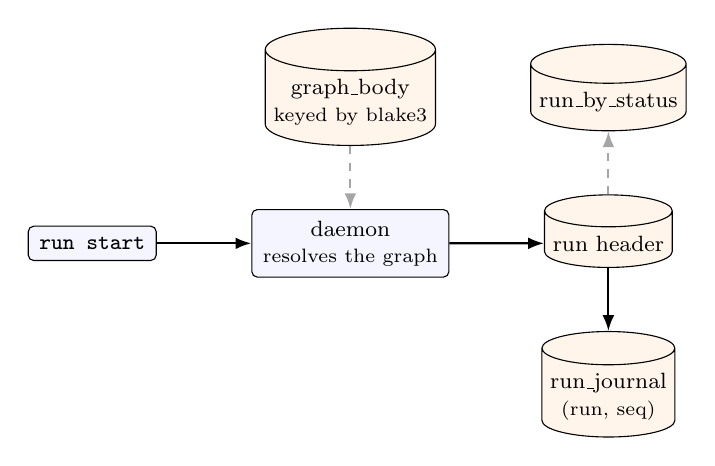
\begin{tikzpicture}[node distance=8mm and 12mm]
  \node[b] (start) {\texttt{run start}};
  \node[b, right=of start] (daemon) {daemon\\\scriptsize resolves the graph};
  \node[s, above=of daemon] (body) {graph\_body\\\scriptsize keyed by blake3};
  \node[s, right=of daemon] (run) {run header};
  \node[s, below=of run] (journal) {run\_journal\\\scriptsize (run, seq)};
  \node[s, above=of run] (status) {run\_by\_status};
  \draw[f] (start) -- (daemon);
  \draw[f] (daemon) -- (run);
  \draw[sf] (body) -- (daemon);
  \draw[f] (run) -- (journal);
  \draw[sf] (run) -- (status);
\end{tikzpicture}}
\captionof{figure}{What \texttt{run start} writes. The graph body is stored once per revision and the header points at its hash, so a run remains readable after the graph file changes.}
\end{minipage}
\end{center}

\subsection*{\texttt{pii graph} --- without the daemon}

\texttt{graph run} and \texttt{graph resume} execute in this process against a store named by
a mandatory \texttt{-{}-db}. They are the offline path: no socket, no daemon, one writer. The
graph is loaded and validated \emph{before} the store is opened, so a refused graph leaves no
store file behind.

\begin{center}
\begin{tabular}{@{}>{\raggedright\arraybackslash}p{0.30\textwidth}>{\raggedright\arraybackslash}p{0.58\textwidth}@{}}
  \toprule
  \textbf{Verb} & \textbf{Flags and effect} \\
  \midrule
  \texttt{lint <file.toml>} & static checks; prints \texttt{OK} plus each inlined node's
    surface, order and origin. Exit 3 on validation errors, 2 on a read or parse failure. \\
  \texttt{check <file.toml>} & the spec-207 name for \texttt{lint}; same code path \\
  \texttt{show <file.toml>} & validate, then print the ASCII topology. A graph that does not
    validate is never rendered. \\
  \texttt{run <file> -{}-db P} & execute and journal. Also \texttt{-{}-run-id},
    \texttt{-{}-input}, \texttt{-{}-allow-write <dir>} (repeatable), \texttt{-{}-no-validate} \\
  \texttt{resume <id> -{}-db P} & replay and continue; \texttt{-{}-allow-write} is repeatable \\
  \texttt{trace <id> -{}-db P [QUERY]} & eight queries over the stored journal (see below) \\
  \texttt{list [-{}-all] [-{}-json] [-{}-dir D] [-{}-repo R]} & installed graphs, their
    revision, their armed-run count and their drift against the repo copy \\
  \texttt{show <name> [-{}-dir D]} & the installed definition, when the name is an installed graph \\
  \texttt{explain <name> [-{}-dir D] [-{}-repo R]} & nodes and ports in execution order \\
  \texttt{edit <name> -{}-file F [-{}-force]} & lint, move the previous file aside, write
    atomically. No verb deletes a graph. \\
  \bottomrule
\end{tabular}
\end{center}

The trace queries are worth memorising, because each answers a question that reading the dump
by eye answers slowly:

\begin{center}
\begin{tabular}{@{}>{\raggedright\arraybackslash}p{0.28\textwidth}>{\raggedright\arraybackslash}p{0.60\textwidth}@{}}
  \toprule
  \textbf{Query} & \textbf{Answers} \\
  \midrule
  (none) & the whole journal, one line per event \\
  \texttt{-{}-count-finished N} & how many times node \texttt{N} finished \\
  \texttt{-{}-node-status N} & the last status recorded for \texttt{N} \\
  \texttt{-{}-max-batch-width} & the widest batch the scheduler executed \\
  \texttt{-{}-terminal} & the run's terminal word \\
  \texttt{-{}-output} & the run's final output value \\
  \texttt{-{}-overlapped A,B} & whether two nodes were ever in flight together \\
  \texttt{-{}-reason N} & why node \texttt{N} ended where it did \\
  \bottomrule
\end{tabular}
\end{center}

\subsection*{\texttt{pii sop}}

A declarative SOP is compiled into the same graph engine; \texttt{run} and \texttt{resume} use
the same journal as \texttt{graph run}. There is no second runner.

\begin{center}
\begin{tabular}{@{}>{\raggedright\arraybackslash}p{0.30\textwidth}>{\raggedright\arraybackslash}p{0.58\textwidth}@{}}
  \toprule
  \textbf{Verb} & \textbf{Effect} \\
  \midrule
  \texttt{compile <f.sop.toml>} & print the graph the SOP compiles to \\
  \texttt{lint <f.sop.toml>} & validate the compiled graph \\
  \texttt{show <f.sop.toml>} & render the compiled topology \\
  \texttt{run <f> -{}-db P} & execute; \texttt{-{}-run-id}, \texttt{-{}-input},
    \texttt{-{}-allow-write} \\
  \texttt{resume <id> -{}-db P} & continue a suspended SOP run \\
  \bottomrule
\end{tabular}
\end{center}

\begin{lstlisting}[language=bash]
pii graph lint graphs/queue.toml                 # static, offline, no store written
pii graph show graphs/night.toml                 # the loaded topology, after weaving
pii run start night --input '{"workdir":"/projects/pi-improved","to":"status"}'
pii run get r000000000261                        # header + coder lines
pii run trace r000000000261 --reason implement   # why the node ended there
pii run resume r000000000261                     # continue after a gate
\end{lstlisting}

\section{The queue}

The queue is a store of work items, one file beside the main store
(\texttt{queue.redb}, tables \texttt{queue\_item} and \texttt{queue\_event}). Each verb is one
RPC; none opens the file.

\begin{center}
\begin{tabular}{@{}>{\raggedright\arraybackslash}p{0.30\textwidth}>{\raggedright\arraybackslash}p{0.58\textwidth}@{}}
  \toprule
  \textbf{Verb} & \textbf{Flags and effect} \\
  \midrule
  \texttt{add} & \texttt{-{}-id}, \texttt{-{}-spec}, \texttt{-{}-title}, \texttt{-{}-criteria}
    (repeatable), \texttt{-{}-touches} (repeatable). Writes one pending item. \\
  \texttt{ls} & every row with its status and reason \\
  \texttt{claim -{}-by <name>} & claim the next pending item for an external worker \\
  \bottomrule
\end{tabular}
\end{center}

An item is \texttt{pending}, \texttt{running}, \texttt{done} or \texttt{parked}. The graph's
\texttt{select} node claims one and writes \texttt{running}; the \texttt{record} node writes
\texttt{done} when the verdict is a pass or the literal \texttt{done}, and \texttt{parked}
with the failing criterion otherwise. A row that stays \texttt{running} is therefore an
operator question, not a bug in the queue: either the run is still alive, or it died holding
the claim.

\begin{center}
\begin{minipage}{\linewidth}
\centering
\resizebox{\linewidth}{!}{%
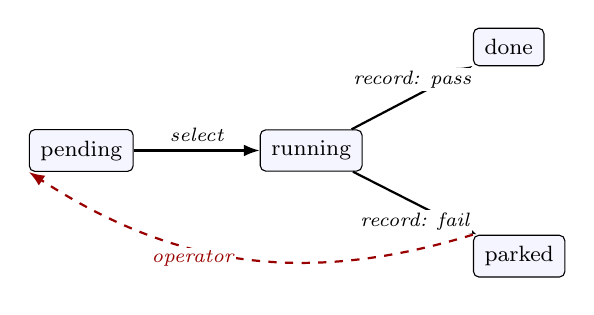
\begin{tikzpicture}[node distance=9mm and 16mm]
  \node[b] (pending) {pending};
  \node[b, right=of pending] (running) {running};
  \node[b, above right=8mm and 14mm of running] (done) {done};
  \node[b, below right=8mm and 14mm of running] (parked) {parked};
  \draw[f] (pending) -- node[p, above=2pt, midway]{select} (running);
  \draw[f] (running) -- node[p, above=2pt, midway]{record: pass} (done);
  \draw[f] (running) -- node[p, below=2pt, midway]{record: fail} (parked);
  \draw[bk] (parked.north west) to[bend left=25] node[p, left=2pt, midway]{operator} (pending.south west);
\end{tikzpicture}}
\captionof{figure}{Four states, two writers. Only \texttt{select} and \texttt{record} move a row; the way back from \texttt{parked} is a person, not a retry loop.}
\end{minipage}
\end{center}

\section{Stores, backups and memory}

\subsection*{\texttt{pii store}}

\begin{center}
\begin{tabular}{@{}>{\raggedright\arraybackslash}p{0.26\textwidth}>{\raggedright\arraybackslash}p{0.62\textwidth}@{}}
  \toprule
  \textbf{Verb} & \textbf{Effect} \\
  \midrule
  \texttt{compact [-{}-dir D]} & offline compaction; prints each file's measured size before
    and after. A store with nothing to reclaim prints a near-equal pair, which is the truth. \\
  \texttt{stats [-{}-dir D]} & one line per table with its row count, then the file's bytes \\
  \texttt{prune [-{}-dir D]} & one retention sweep under the default policy, then the count.
    Finished runs older than 30 days go, node events older than 7 days go first, at most
    1{,}000 rows per sweep. A \texttt{Running} or \texttt{Suspended} run is never touched. \\
  \bottomrule
\end{tabular}
\end{center}

\texttt{compact} and \texttt{prune} open the store directly and therefore need the daemon
stopped. \texttt{stats} does too, for the same reason; run it against a copy if the daemon
must stay up.

\subsection*{\texttt{pii backup} and \texttt{pii restore}}

Both are offline for the same reason, and both print a manifest line per file with its byte
count, format version and blake3 digest.

\begin{lstlisting}[language=bash]
pii backup /var/backups/pii-$(date +%F) --dir /var/lib/pii
pii restore /var/backups/pii-2026-11-04 --dir /var/lib/pii --force
\end{lstlisting}

\texttt{restore} refuses to overwrite a non-empty target unless \texttt{-{}-force} is given.

\subsection*{\texttt{pii memory}}

The memory family is the widest in the binary, and its subcommands split into three kinds:
text search, the entity graph, and lifecycle.

\begin{longtable}{@{}>{\raggedright\arraybackslash}p{0.28\textwidth}>{\raggedright\arraybackslash}p{0.58\textwidth}@{}}
  \toprule
  \textbf{Verb} & \textbf{Flags and effect} \\
  \midrule
  \endhead
  \texttt{search <q>} & \texttt{-{}-k N} (default 6). BM25 over the document table; no model. \\
  \texttt{put <text>} & \texttt{-{}-layer L} (default \texttt{l1}), \texttt{-{}-kind K}
    (default \texttt{atom}). One document, written once. \\
  \texttt{learn} & \texttt{-{}-run}, \texttt{-{}-status}, \texttt{-{}-reason} (required);
    \texttt{-{}-graph}, \texttt{-{}-attempts}, \texttt{-{}-session}, \texttt{-{}-commit}.
    Writes an outcome as an \texttt{atom}; the key is run+status+reason, so a retried report
    is \texttt{unchanged}. \\
  \texttt{consolidate} & fold recent atoms into longer documents \\
  \texttt{entity add} & \texttt{-{}-kind}, \texttt{-{}-name}, \texttt{-{}-source} (repeatable,
    \texttt{run:}/\texttt{file:}/\texttt{actor:}), \texttt{-{}-attr k=v} \\
  \texttt{entity show <id>} & one record, its tier, and why it holds that tier \\
  \texttt{entity list} & \texttt{-{}-kind K} or \texttt{-{}-name N}; \texttt{-{}-limit},
    \texttt{-{}-rank} \\
  \texttt{link <from> <to>} & \texttt{-{}-kind} or \texttt{-{}-rel}, \texttt{-{}-source},
    \texttt{-{}-attr} \\
  \texttt{neighbours <id>} & \texttt{-{}-depth} (default 1, capped by config),
    \texttt{-{}-limit} \\
  \texttt{compact} & compact \texttt{memory.redb}; daemon stopped \\
  \texttt{show <id>} & one document with its tier and reason \\
  \texttt{tiers} & counts per tier, and the policy in force \\
  \texttt{archive} & \texttt{-{}-before <epoch|Ns|Nm|Nh|Nd ago>}; writes
    \texttt{<dir>/memory/archive-<ts>.jsonl} \\
  \texttt{restore} & bring archived documents back into the live tables \\
  \bottomrule
\end{longtable}

Every graph bound is also a flag, so a one-off query can be narrowed without editing the
config: \texttt{-{}-max-entities}, \texttt{-{}-max-relationships}, \texttt{-{}-max-provenance},
\texttt{-{}-max-depth}, \texttt{-{}-max-results}, \texttt{-{}-max-bytes}. The tier policy has
\texttt{-{}-hot-secs}, \texttt{-{}-warm-secs} and \texttt{-{}-hot-count}. A bound that is
exceeded is refused by name (\texttt{entity\_cap}, \texttt{result\_cap}, \texttt{bytes\_cap}),
never truncated silently.

\begin{center}
\begin{minipage}{\linewidth}
\centering
\resizebox{\linewidth}{!}{%
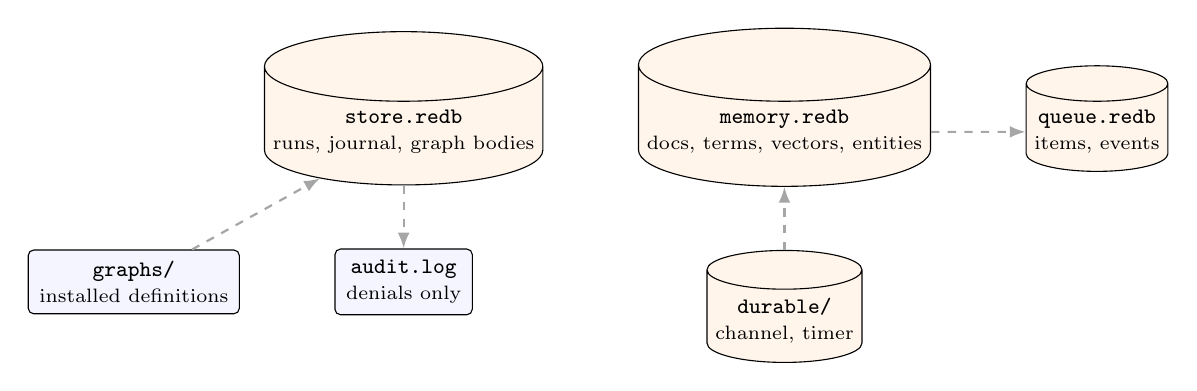
\begin{tikzpicture}[node distance=8mm and 12mm]
  \node[s] (store) {\texttt{store.redb}\\\scriptsize runs, journal, graph bodies};
  \node[s, right=of store] (mem) {\texttt{memory.redb}\\\scriptsize docs, terms, vectors, entities};
  \node[s, right=of mem] (queue) {\texttt{queue.redb}\\\scriptsize items, events};
  \node[s, below=of mem] (durable) {\texttt{durable/}\\\scriptsize channel, timer};
  \node[b, below=of store] (audit) {\texttt{audit.log}\\\scriptsize denials only};
  \node[b, left=of audit] (graphs) {\texttt{graphs/}\\\scriptsize installed definitions};
  \draw[sf] (store) -- (audit);
  \draw[sf] (mem) -- (queue);
  \draw[sf] (durable) -- (mem);
  \draw[sf] (graphs) -- (store);
\end{tikzpicture}}
\captionof{figure}{What an installation actually holds. The main store, the memory store, the queue and the durable area are separate redb files; the audit trail is a text file because it must remain readable when a store is not.}
\end{minipage}
\end{center}

\section{Knowledge, skills and indices}

\begin{center}
\begin{tabular}{@{}>{\raggedright\arraybackslash}p{0.24\textwidth}>{\raggedright\arraybackslash}p{0.64\textwidth}@{}}
  \toprule
  \textbf{Verb} & \textbf{Flags and effect} \\
  \midrule
  \texttt{learn scan} & \texttt{-{}-traj}, \texttt{-{}-min-runs}, \texttt{-{}-outlier-factor},
    \texttt{-{}-max-files}, \texttt{-{}-max-file-bytes}. Reads trajectories, proposes
    candidate lessons. \\
  \texttt{learn list}, \texttt{learn show <id>} & the candidate table, one candidate \\
  \texttt{learn verify} & \texttt{<id>} or \texttt{-{}-all}; \texttt{-{}-max-runs} (5),
    \texttt{-{}-run-ms} (30000), \texttt{-{}-scratch}, \texttt{-{}-protect} (repeatable),
    \texttt{-{}-input}. Re-runs the evidence in a scratch tree. \\
  \texttt{learn promote} & requires \texttt{-{}-metric graph\_definition\_changed} and
    \texttt{-{}-window-secs}; \texttt{-{}-kind quarantine\_graph}, \texttt{-{}-ttl-secs},
    \texttt{-{}-actor} \\
  \texttt{learn promotions} & \texttt{-{}-sweep} to expire lapsed promotions \\
  \texttt{learn revert <id>} & take a promotion back, with an actor and a ledger row \\
  \texttt{learn ledger} & \texttt{-{}-tail N}; the append-only record of every promotion \\
  \texttt{skill add} & \texttt{-{}-file}, \texttt{-{}-layer L1|L2|L3}. The pinned script is
    hashed where it lies and never executed. \\
  \texttt{skill list} & \texttt{-{}-all}, \texttt{-{}-layer} \\
  \texttt{skill show}, \texttt{skill explain} & one skill; \texttt{explain} renders the
    \texttt{WHEN TO USE}, \texttt{CONTRACT} and \texttt{VERBS} sections verbatim \\
  \texttt{skill edit <id>} & \texttt{-{}-file}, \texttt{-{}-note}; records the commit or file
    and time as evidence \\
  \texttt{index code} & \texttt{-{}-root}, \texttt{-{}-max}, \texttt{-{}-dir},
    \texttt{-{}-no-docs}; skips \texttt{target}, \texttt{\_tmp} and \texttt{vendor} \\
  \texttt{index docs} & \texttt{-{}-root}, \texttt{-{}-kind spec|handoff|ops|all}; one
    document per spec, per \texttt{HANDOFF} section, per operations doc \\
  \bottomrule
\end{tabular}
\end{center}

\texttt{index docs} is idempotent by construction: a document's id is the hash of its text, so
a second pass over unchanged files reports \texttt{unchanged} and writes nothing.

\section{Observation and decisions}

\begin{center}
\begin{tabular}{@{}>{\raggedright\arraybackslash}p{0.24\textwidth}>{\raggedright\arraybackslash}p{0.64\textwidth}@{}}
  \toprule
  \textbf{Verb} & \textbf{Flags and effect} \\
  \midrule
  \texttt{health} & \texttt{-{}-json}. Exit 0 when the daemon answers from this client's
    revision, 2 when nothing answers, 3 on drift or an unprovable comparison. \\
  \texttt{metrics} & the gauge and counter text format, one line per series \\
  \texttt{sys status}, \texttt{sys reload} & the status payload; re-read the config and the
    project layer without a restart \\
  \texttt{disk} & \texttt{-{}-root <repo>}; artefact roots with bytes, age, filesystem, then
    free space for \texttt{/} and for the repository's volume. Read-only. \\
  \texttt{incidents scan} & \texttt{-{}-root}, \texttt{-{}-new}; or
    \texttt{-{}-source runtime -{}-log F} for the daemon's own log, with
    \texttt{-{}-ingest -{}-dir D} to store what it found \\
  \texttt{incidents show} & \texttt{-{}-dir}, \texttt{-{}-id} \\
  \texttt{incidents distance} & \texttt{-{}-since YYYY-MM-DD} \\
  \texttt{loop emit} & \texttt{-{}-cycle}, \texttt{-{}-kind}, \texttt{-{}-detail},
    \texttt{-{}-file}. Always records locally; exit 3 if the daemon did not answer, so the
    caller can record the gap. \\
  \texttt{loop events} & \texttt{-{}-last N} (20), \texttt{-{}-file}, \texttt{-{}-log} \\
  \texttt{cron ls} & configured cron entries \\
  \texttt{approve ls} & pending approvals \\
  \texttt{approve allow|deny <id>} & \texttt{-{}-note}; resolves one gate \\
  \texttt{heal ls}, \texttt{heal show <sig>} & the heal-attempt ledger, one signature \\
  \texttt{net ls} & the listeners the daemon reports \\
  \texttt{worker ls}, \texttt{worker reload <name>} & supervised children; drain and reload \\
  \texttt{treat export} & \texttt{-{}-out <dir>}; writes \texttt{manifest.json},
    \texttt{fix.patch}, \texttt{repro.sh} \\
  \texttt{treat import}, \texttt{apply}, \texttt{list} & \texttt{-{}-check},
    \texttt{-{}-is-ancestor}, \texttt{-{}-yes} \\
  \texttt{deploy-card render} & \texttt{-{}-card F; refuses a card missing any of the five
    fields, naming the field} \\
  \texttt{deploy-card approve} & \texttt{-{}-card F -{}-rev R}; bound to the revision the card
    names \\
  \texttt{deploy-card refuse} & \texttt{-{}-card F [-{}-reason T]} \\
  \bottomrule
\end{tabular}
\end{center}

Every deploy-card decision appends one line to the operator acts file, whose default is
\texttt{\_tmp/autonomy/operator-acts.log} and whose path is overridable with
\texttt{\$PII\_ACTS}. That file is the evidence the distance metric counts; a decision that is
not in it did not happen.

\section{Devices, sandboxes and scaffolding}

\begin{center}
\begin{tabular}{@{}>{\raggedright\arraybackslash}p{0.24\textwidth}>{\raggedright\arraybackslash}p{0.64\textwidth}@{}}
  \toprule
  \textbf{Verb} & \textbf{Flags and effect} \\
  \midrule
  \texttt{mqtt ls} & devices, from their own discovery messages \\
  \texttt{mqtt sub <filter> [secs]} & what a filter carries, for a bounded window \\
  \texttt{mqtt pub <topic> <text>} & \texttt{-{}-qos 0|1|2}, \texttt{-{}-retain} \\
  \texttt{mqtt send <device> <cmd>} & address a device by name, not by topic \\
  \texttt{sandbox-exec} & \texttt{-{}-profile <p> -{}-workspace <d> -{}- <argv>}; applies
    Landlock, verifies enforcement, then execs \\
  \texttt{worker-exec} & the reference worker on stdio; ops \texttt{echo}, \texttt{sleep},
    \texttt{crash}, \texttt{info} \\
  \texttt{tui} & \texttt{-{}-connect auto|loopback|<socket>}, \texttt{-{}-sandbox},
    \texttt{-{}-workspace}. Never auto-starts a daemon. \\
  \texttt{project init <dir>} & writes \texttt{.pii/settings.toml}, \texttt{.pii/policy.toml},
    \texttt{.pi/}, \texttt{.claude/} and five \texttt{.gitignore} lines; refuses a target that
    already holds a credential \\
  \texttt{lane plan <N>} & \texttt{-{}-resume <sid>}, \texttt{-{}-dry-run}; prints the agent,
    model, provider, spec, brief, log and wait, and writes nothing when dry \\
  \texttt{lane run <N>} & the same plan, then the run \\
  \texttt{lane rev} & the revision the lane binary was built from \\
  \texttt{soak} & \texttt{-{}-connect <socket> -{}-runs N -{}-graph G
    [-{}-concurrency C]; N runs against a live daemon} \\
  \bottomrule
\end{tabular}
\end{center}

\texttt{mqtt} reads the broker from \texttt{-{}-url}, else from \texttt{\$PII\_MQTT\_URL}, and
otherwise uses the loopback broker on port 1883. Its output is one JSON object per call --- the same shape the
model's tool returns --- so a script and an agent see the same thing.

\section{Exit codes}

The binary uses a small, stable set. Scripts depend on these, and a change to one is a
breaking change.

\begin{longtable}{@{}>{\raggedright\arraybackslash}p{0.10\textwidth}>{\raggedright\arraybackslash}p{0.78\textwidth}@{}}
  \toprule
  \textbf{Code} & \textbf{Meaning} \\
  \midrule
  \endhead
  0 & success \\
  2 & usage error, a refused control call, or an unreadable store. The message names the
      argument or the call. \\
  3 & the work ran and did not pass: graph validation errors, \texttt{health} drift or an
      unprovable revision comparison, \texttt{loop emit} with the daemon down \\
  4 & the sandbox profile could not be enforced; the daemon refuses to start unconfined \\
  8 & the lane's dirty-tree stop; the tree has changes the run did not make \\
  \bottomrule
\end{longtable}

\begin{center}
\begin{minipage}{\linewidth}
\centering
\resizebox{\linewidth}{!}{%
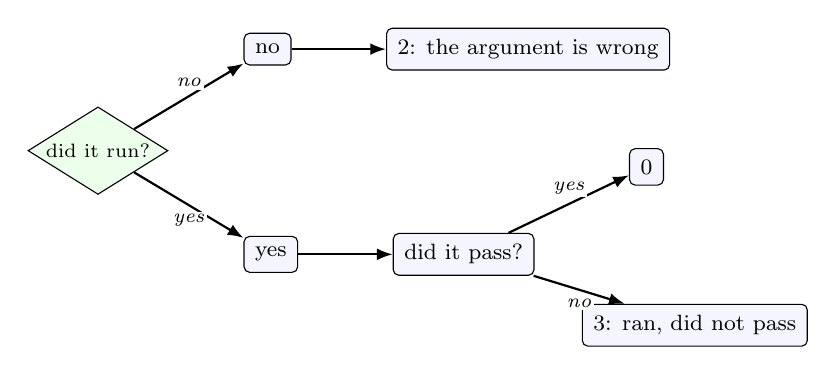
\begin{tikzpicture}[node distance=8mm and 12mm]
  \node[v] (ask) {did it run?};
  \node[b, above right=8mm and 14mm of ask] (no) {no};
  \node[b, below right=8mm and 14mm of ask] (yes) {yes};
  \node[b, right=of no] (usage) {2: the argument is wrong};
  \node[b, right=of yes] (verdict) {did it pass?};
  \node[b, above right=6mm and 12mm of verdict] (pass) {0};
  \node[b, right=6mm of verdict, yshift=-9mm] (fail) {3: ran, did not pass};
  \draw[f] (ask) -- node[p, above=2pt, midway]{no} (no);
  \draw[f] (ask) -- node[p, below=2pt, midway]{yes} (yes);
  \draw[f] (no) -- (usage);
  \draw[f] (yes) -- (verdict);
  \draw[f] (verdict) -- node[p, above=2pt, midway]{yes} (pass);
  \draw[f] (verdict) -- node[p, below=2pt, midway]{no} (fail);
\end{tikzpicture}}
\captionof{figure}{The decision an exit code encodes. \enquote{Ran and did not pass} is deliberately distinct from \enquote{did not run}: a script that retries on 3 and reports on 2 is doing different things, and should say so.}
\end{minipage}
\end{center}

\begin{lstlisting}[language=bash]
pii health >/dev/null; echo $?      # 0 same build, 3 drift, 2 no daemon
pii graph lint graphs/night.toml    # 0 ok, 3 invalid, 2 unreadable
pii store stats --dir /var/lib/pii  # needs the daemon stopped
pii metrics | grep pii_store_bytes  # one series per store file
\end{lstlisting}
\chapter{Configuration}

\label{ch:config}

This chapter answers what the daemon reads at start, which of two files wins when both set
the same key, what it refuses to read at all, and how to change a setting without a restart.
It also states where every file an installation writes actually lives, because the most
common configuration fault is not a wrong value --- it is a second daemon reading different
files from the one the operator is looking at.

\section{Two files, one effective config}

There is a global file and, optionally, a project file. The global file is the one an
operator edits for a host; the project file is the one a repository carries, and it may set
only the settings a repository has any business setting.

\begin{center}
\begin{minipage}{\linewidth}
\centering
\resizebox{\linewidth}{!}{%
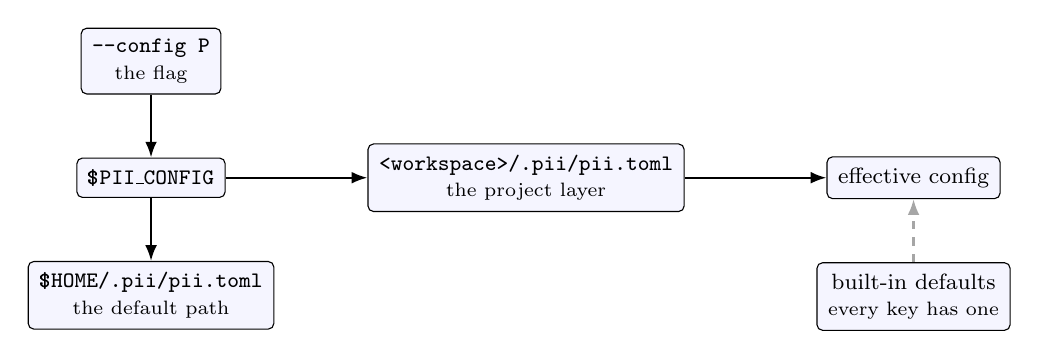
\begin{tikzpicture}[node distance=8mm and 12mm]
  \node[b] (flag) {\texttt{-{}-config P}\\\scriptsize the flag};
  \node[b, below=of flag] (env) {\texttt{\$PII\_CONFIG}};
  \node[b, below=of env] (def) {\texttt{\$HOME/.pii/pii.toml}\\\scriptsize the default path};
  \node[b, right=of env, xshift=6mm] (proj) {\texttt{<workspace>/.pii/pii.toml}\\\scriptsize the project layer};
  \node[b, right=of proj, xshift=6mm] (eff) {effective config};
  \node[b, below=of eff] (defaults) {built-in defaults\\\scriptsize every key has one};
  \draw[f] (flag) -- (env);
  \draw[f] (env) -- (def);
  \draw[f] (env) -- (proj);
  \draw[sf] (defaults) -- (eff);
  \draw[f] (proj) -- (eff);
\end{tikzpicture}}
\captionof{figure}{Resolution order. The first of flag, \texttt{\$PII\_CONFIG} and the default path decides which global file is read; the project file is then layered over it, and every unset key falls through to a built-in default.}
\end{minipage}
\end{center}

The default path is \texttt{\$HOME/.pii/pii.toml}, and it is resolved \emph{before} the runtime
directory. That ordering is deliberate: \texttt{[core].runtime\_dir} lives in the file that
sets it, so a config path derived from the runtime directory would be circular.

A file that does not exist is not an error at the default path: the daemon starts with
built-in defaults and then refuses on the missing model. The same is true of a
\texttt{-{}-config} path that does not exist, which is worth knowing: a typo in the flag does
not say \enquote{no such file}, it says \enquote{no model configured} a moment later.

\section{The project layer, and what it may not say}

A workspace may carry \texttt{<workspace>/.pii/pii.toml}. It is read at start and on
\texttt{pii sys reload}, through one function, so the two can never disagree about which file
is read. A project file that exists but does not parse is fatal; it never silently falls back
to the global file.

The merge is not a general merge. A project value wins for three things only:

\begin{center}
\begin{tabular}{@{}>{\raggedright\arraybackslash}p{0.30\textwidth}>{\raggedright\arraybackslash}p{0.58\textwidth}@{}}
  \toprule
  \textbf{Project may set} & \textbf{Why it is safe} \\
  \midrule
  \texttt{[core].model} & the model a repository's work should use \\
  \texttt{[llama].host} & where that model is served, per repository \\
  \texttt{[[model\_tier]]} & the routing table, replaced whole rather than merged \\
  \bottomrule
\end{tabular}
\end{center}

Everything else that decides where the daemon writes or what it may reach is refused, and the
refusal names the setting:

\begin{lstlisting}[language=bash]
error: project config sets global-only settings: [net], grant_ceiling,
[core].runtime_dir (only the global ~/.pii/pii.toml may set them)
\end{lstlisting}

The list is short and closed: \texttt{[net]}, \texttt{grant\_ceiling},
\texttt{[core].runtime\_dir}, \texttt{[core].log\_file}, \texttt{[core].audit} and
\texttt{[core].observer}. The reason is asymmetric risk. A repository that could widen
\texttt{[net] grants} would let a checkout grant itself egress; a repository that could move
\texttt{runtime\_dir} would point a daemon at a store nobody is watching. A model id, by
contrast, is exactly the kind of thing that should differ per project.

\begin{center}
\begin{minipage}{\linewidth}
\centering
\resizebox{\linewidth}{!}{%
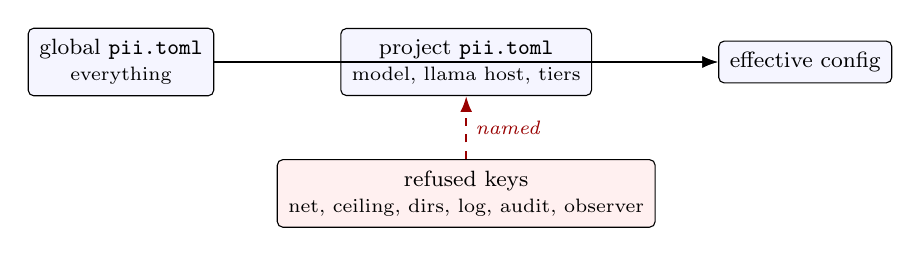
\begin{tikzpicture}[node distance=8mm and 16mm]
  \node[b] (global) {global \texttt{pii.toml}\\\scriptsize everything};
  \node[b, right=of global] (project) {project \texttt{pii.toml}\\\scriptsize model, llama host, tiers};
  \node[b, right=of project] (eff) {effective config};
  \node[b, below=of project, fill=red!6] (refused) {refused keys\\\scriptsize net, ceiling, dirs, log, audit, observer};
  \draw[f] (global) -- (eff);
  \draw[f] (project) -- (eff);
  \draw[bk] (refused) -- node[p, right=2pt, midway]{named} (project);
\end{tikzpicture}}
\captionof{figure}{The layer is a whitelist, not a patch. A project file is a set of opinions about models; anything that decides where bytes land belongs to the host.}
\end{minipage}
\end{center}

\section{The file is strict}

Every section is deserialised with unknown fields denied. A misspelled key is a load error
that names the key, not a setting that silently does nothing. This is a security property
rather than a style: \texttt{sandbx = "workspace"} must not start an unconfined daemon.

Two refusals are worth their own paragraph because they have been hit in practice:

\begin{itemize}
  \item \texttt{[core].ollama\_host} is refused by name. The ollama provider was retired; the
    key is not merely unknown, it produces a message that says to set \texttt{[llama] host}
    instead.
  \item Two \texttt{[[model\_tier]]} entries with the same name, or an entry with an empty
    name or model, fail validation before the daemon binds a socket.
\end{itemize}

\section{The sections}

\begin{longtable}{@{}>{\raggedright\arraybackslash}p{0.24\textwidth}>{\raggedright\arraybackslash}p{0.64\textwidth}@{}}
  \toprule
  \textbf{Key} & \textbf{What it decides} \\
  \midrule
  \endhead
  \texttt{grant\_ceiling} & capability names no graph or node may request beyond; empty means
    no ceiling. An unknown capability name is an error. This is the one setting a graph
    author cannot argue with. \\
  \texttt{[core]} & the host's own settings: model, directories, log, switches \\
  \texttt{[llama]} & where \texttt{llamacpp-server:} models dial; default
    \texttt{http://127.0.0.1:8080/v1} \\
  \texttt{[net]} & egress policy: \texttt{grants} (host:port patterns) and
    \texttt{allow\_private}. Default: no grants at all. \\
  \texttt{[[worker]]} & a supervised child: \texttt{name}, \texttt{program},
    \texttt{args}, \texttt{env}, \texttt{max\_in\_flight} \\
  \texttt{[[channel]]} & an inbound message source and the graph it starts per message \\
  \texttt{[[mqtt]]} & one broker connection and the graph each message starts \\
  \texttt{[hal]} & hardware backend (\texttt{sim} or \texttt{gpiod}) and the pins, I2C and
    SPI a graph may claim. Absent = the HAL is off and a \texttt{hal} node fails. \\
  \texttt{[wasm]} & plugin host: the one directory modules load from, plus per-call
    \texttt{timeout\_ms}, \texttt{max\_memory\_mib} and \texttt{fuel}. Absent = off. \\
  \texttt{[memory]} & \texttt{path}; empty means the store beside the main store \\
  \texttt{[memory\_graph]} & the bounds on the entity graph and the tier policy \\
  \texttt{[[cron]]} & a named timer entry: \texttt{name}, \texttt{graph},
    \texttt{schedule}, \texttt{input} \\
  \texttt{[[model\_tier]]} & a named model: \texttt{name}, \texttt{model},
    \texttt{tools}, \texttt{max\_tokens} \\
  \texttt{[evolve.routing]} & step to model, for the steps \texttt{localize},
    \texttt{patch}, \texttt{review}, \texttt{research}, \texttt{orchestrator}. A typo'd step
    is an error, not a silent no-route. \\
  \bottomrule
\end{longtable}

\subsection*{\texttt{[core]}}

\begin{longtable}{@{}>{\raggedright\arraybackslash}p{0.27\textwidth}>{\raggedright\arraybackslash}p{0.45\textwidth}>{\raggedright\arraybackslash}p{0.18\textwidth}@{}}
  \toprule
  \textbf{Key} & \textbf{Meaning} & \textbf{Default} \\
  \midrule
  \endhead
  \texttt{model} & the model spec runs use when a graph names none & none \\
  \texttt{runtime\_dir} & sockets, installed graphs, crashes & per-uid \\
  \texttt{durable\_dir} & channel, timer and other durable stores & state\texttt{/durable} \\
  \texttt{session\_runs\_cap} & runs remembered per session in memory & built-in cap \\
  \texttt{trajectory\_dir} & when set, each run appends a JSONL trajectory & off \\
  \texttt{trajectory\_max\_bytes} & aggregate bound on the trajectory directory & 512 MiB \\
  \texttt{trajectory\_max\_files} & aggregate file bound & 50{,}000 \\
  \texttt{learn\_interval\_secs} & the unattended learn pass interval & 86{,}400 \\
  \texttt{log\_file} & daemon events as JSON lines & off \\
  \texttt{log\_rotate\_bytes} & rotate before a line passes this size & 10{,}485{,}760 \\
  \texttt{log\_keep\_files} & rotated files kept beside the live one & 5 \\
  \texttt{observer} & \texttt{on}/\texttt{off}; measurement only & \texttt{on} \\
  \texttt{audit} & \texttt{on}/\texttt{off}; measurement only & \texttt{on} \\
  \bottomrule
\end{longtable}

Three keys read a zero in a way that is easy to guess wrong, so they are stated here rather
than left to the sample. \texttt{learn\_interval\_secs = 0} switches the unattended learn
pass off; the field is optional and its absence means every 86{,}400 seconds.
\texttt{trajectory\_max\_bytes} and \texttt{trajectory\_max\_files} treat a zero as
\enquote{unset} and fall back to the defaults, never as \enquote{unbounded}, because the
trajectory directory is always bounded. \texttt{log\_rotate\_bytes = 0} is different again:
it is passed through, and the sample documents it as \enquote{never rotate} --- which is a
legitimate choice for a log a supervisor already rotates, and a bad one for a host nobody
watches.

The two measurement switches deserve a warning that the file cannot give: switching
\texttt{audit} off stops denials reaching \texttt{audit.log}, and switching \texttt{observer}
off detaches tool-call, store and provider logging. Both announce themselves as warning
events at start, and both are documented as measurement-only. An installation that runs with
either off is not observably the same installation as one that runs with them on.

\subsection*{\texttt{[memory\_graph]}}

These bounds are also command-line flags on \texttt{pii memory}, so a one-off query can be
narrowed without touching the file.

\begin{center}
\begin{tabular}{@{}>{\raggedright\arraybackslash}p{0.26\textwidth}>{\raggedright\arraybackslash}p{0.16\textwidth}>{\raggedright\arraybackslash}p{0.46\textwidth}@{}}
  \toprule
  \textbf{Key} & \textbf{Default} & \textbf{Refusal when exceeded} \\
  \midrule
  \texttt{max\_entities} & 10{,}000 & \texttt{entity\_cap} \\
  \texttt{max\_relationships} & 50{,}000 & \texttt{relationship\_cap} \\
  \texttt{max\_provenance} & 32 & \texttt{provenance\_cap} \\
  \texttt{max\_attributes} & 32 & none; the extra attribute is refused \\
  \texttt{max\_depth} & 3 & depth clamp at the call \\
  \texttt{default\_depth} & 1 & --- \\
  \texttt{max\_results} & 200 & \texttt{result\_cap} \\
  \texttt{hot\_secs} & 86{,}400 & tier policy \\
  \texttt{warm\_secs} & 604{,}800 & tier policy \\
  \texttt{hot\_count} & 10 & tier policy \\
  \texttt{max\_bytes} & 16 MiB & \texttt{bytes\_cap} \\
  \bottomrule
\end{tabular}
\end{center}

\section{Where the files are}

Three directories, and they are not interchangeable. The state directory holds what must
survive; the runtime directory holds what a restart may rebuild; the workspace is what the
sandbox confines writes to.

\begin{center}
\begin{minipage}{\linewidth}
\centering
\resizebox{\linewidth}{!}{%
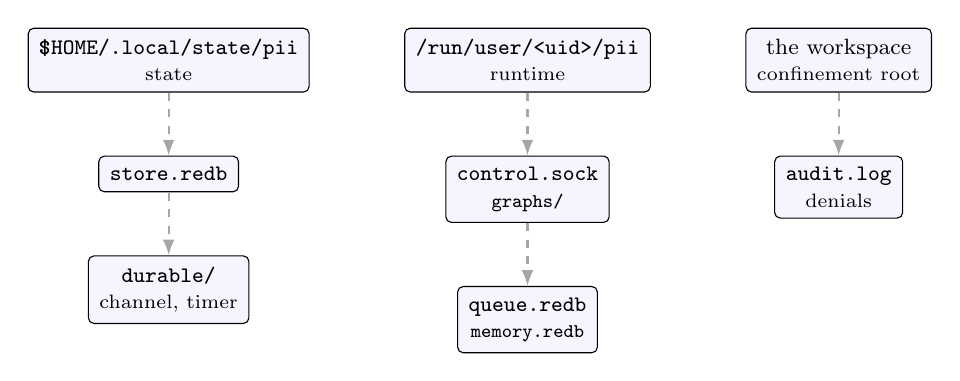
\begin{tikzpicture}[node distance=8mm and 12mm]
  \node[b] (state) {\texttt{\$HOME/.local/state/pii}\\\scriptsize state};
  \node[b, right=of state] (run) {\texttt{/run/user/<uid>/pii}\\\scriptsize runtime};
  \node[b, right=of run] (ws) {the workspace\\\scriptsize confinement root};
  \node[b, below=of state] (store) {\texttt{store.redb}};
  \node[b, below=of run] (sock) {\texttt{control.sock}\\\scriptsize \texttt{graphs/}};
  \node[b, below=of ws] (audit) {\texttt{audit.log}\\\scriptsize denials};
  \node[b, below=of store] (dur) {\texttt{durable/}\\\scriptsize channel, timer};
  \node[b, below=of sock] (sib) {\texttt{queue.redb}\\\scriptsize \texttt{memory.redb}};
  \draw[sf] (state) -- (store);
  \draw[sf] (run) -- (sock);
  \draw[sf] (ws) -- (audit);
  \draw[sf] (store) -- (dur);
  \draw[sf] (sock) -- (sib);
\end{tikzpicture}}
\captionof{figure}{The layout an operator has to hold in mind. The audit trail lives beside the store, not in the log directory, so it survives losing a log volume.}
\end{minipage}
\end{center}

\begin{center}
\begin{tabular}{@{}>{\raggedright\arraybackslash}p{0.30\textwidth}>{\raggedright\arraybackslash}p{0.58\textwidth}@{}}
  \toprule
  \textbf{Path} & \textbf{Contents and note} \\
  \midrule
  \texttt{\$PII\_STATE\_DIR} & the state directory; default
    \texttt{\$HOME/.local/state/pii} \\
  \texttt{\$PII\_RUNTIME\_DIR} & sockets and ephemeral files; default
    \texttt{/run/user/<uid>/pii} \\
  \texttt{store.redb} & the main store, in the runtime or state dir; \texttt{-{}-store}
    overrides \\
  \texttt{audit.log} & beside the store: denials and the sandbox profile in force, rotated
    like the log \\
  \texttt{queue.redb} & beside the store: the queue's items and events \\
  \texttt{memory.redb} & beside the store: documents and the entity graph \\
  \texttt{durable/channel.redb} & under the state dir: channel cursors and last started runs \\
  \texttt{durable/timer.redb} & under the state dir: the timer wheel \\
  \texttt{graphs/} & under the runtime dir: installed definitions, \texttt{<name>.toml} \\
  \texttt{./graphs} & the repository copy that \texttt{graph list} compares against \\
  \bottomrule
\end{tabular}
\end{center}

\texttt{pii graph list} prints \texttt{DRIFT} when the installed copy differs from the
repository copy, which is the fastest way to answer \enquote{is the daemon running what I
reviewed}.

\section{Secrets are not configuration}

No credential is a config value. The file names the \emph{variable} or the \emph{file} that
holds a secret, never the secret:

\begin{itemize}
  \item \texttt{[[channel]]} uses \texttt{token\_env} or \texttt{token\_file}, and
    \texttt{secret\_env} or \texttt{secret\_file} for webhook signatures.
  \item \texttt{[[mqtt]]} uses \texttt{username\_env} or \texttt{username\_file}, and
    \texttt{password\_env} or \texttt{password\_file}. Credentials in clear text to a
    non-loopback broker are refused unless \texttt{allow\_plaintext\_credentials} is true.
  \item Provider keys come from \texttt{OPENAI\_API\_KEY}, \texttt{ANTHROPIC\_API\_KEY} or
    \texttt{GEMINI\_API\_KEY} in the daemon's environment, and are scrubbed from provider
    errors and events.
\end{itemize}

The reason is not tidiness. A config file is copied into backups, printed in bug reports and
mounted into containers; an environment variable is not. The scrubber that removes
secret-named variables from log lines is built from the daemon's own environment, so a key
passed as a \texttt{-{}-config} value would be invisible to it.

\section{Environment variables}

\begin{longtable}{@{}>{\raggedright\arraybackslash}p{0.28\textwidth}>{\raggedright\arraybackslash}p{0.60\textwidth}@{}}
  \toprule
  \textbf{Variable} & \textbf{Effect} \\
  \midrule
  \endhead
  \texttt{PII\_CONFIG} & the config file, overriding the default path \\
  \texttt{PII\_STATE\_DIR} & the state directory \\
  \texttt{PII\_RUNTIME\_DIR} & the runtime directory; wins over
    \texttt{[core].runtime\_dir} \\
  \texttt{PII\_MODEL} & the model when \texttt{[core].model} is unset; the flag or the file
    wins \\
  \texttt{PII\_TRAJECTORY\_DIR} & trajectory output; overrides
    \texttt{[core].trajectory\_dir} \\
  \texttt{PII\_MQTT\_URL} & broker for \texttt{pii mqtt}, after \texttt{-{}-url} \\
  \texttt{PII\_ACTS} & the operator acts file the deploy-card and distance commands append to \\
  \texttt{PII\_LOOP\_EVENTS} & the loop event NDJSON file \\
  \texttt{PII\_AGENT} & the lane's agent: \texttt{claude} or \texttt{pi} \\
  \texttt{PII\_GRAPH\_EDIT\_OK} & permits graph edits from the spec lane \\
  \texttt{ALLOW\_DIRTY} & permits the lane to start on a dirty tree, for a resume \\
  \texttt{OPENAI\_BASE\_URL} & an OpenAI-compatible endpoint; any vendor with that shape \\
  \texttt{OPENAI\_API\_KEY} & its key; optional for a local server \\
  \texttt{ANTHROPIC\_BASE\_URL} & default \texttt{https://api.anthropic.com} \\
  \texttt{ANTHROPIC\_API\_KEY} & required for Anthropic models \\
  \texttt{GEMINI\_BASE\_URL} & the Google endpoint; the default is the public host \\
  \texttt{GEMINI\_API\_KEY} & sent as \texttt{x-goog-api-key}, never in the URL \\
  \bottomrule
\end{longtable}

\section{Changing a setting}

There are three cost levels, and choosing the wrong one is how a host ends up running a
config nobody edited.

\begin{center}
\begin{minipage}{\linewidth}
\centering
\resizebox{\linewidth}{!}{%
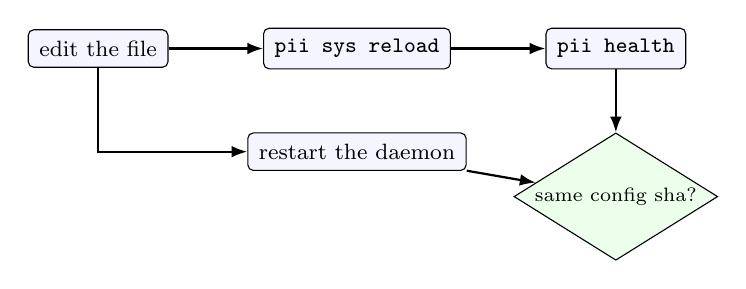
\begin{tikzpicture}[node distance=8mm and 12mm]
  \node[b] (edit) {edit the file};
  \node[b, right=of edit] (reload) {\texttt{pii sys reload}};
  \node[b, right=of reload] (status) {\texttt{pii health}};
  \node[b, below=of reload] (restart) {restart the daemon};
  \node[v, below=of status] (ok) {same config sha?};
  \draw[f] (edit) -- (reload);
  \draw[f] (reload) -- (status);
  \draw[f] (edit) |- (restart);
  \draw[f] (restart) -- (ok);
  \draw[f] (status) -- (ok);
\end{tikzpicture}}
\captionof{figure}{A change is not in force until a surface says so. \texttt{pii health} prints the config path and a sha256 of the file it read, which is the only proof that the daemon is running the file you edited.}
\end{minipage}
\end{center}

\texttt{pii health} prints, on its first three lines, the binary's version, target and
revision, this client's revision, and the config path with its digest:

\begin{lstlisting}[language=bash]
pii 0.2.0 (c05f3d1e4dd3, x86_64-unknown-linux-gnu)
client: c05f3d1e4dd3
config: /root/.pii/pii.toml sha256=9f2c...
\end{lstlisting}

If the digest is not the file you just saved, the daemon read a different file: check
\texttt{\$PII\_CONFIG} in the service unit before editing anything else.

\texttt{pii sys reload} is narrower than its name suggests, and knowing its exact scope saves
an afternoon. It re-reads the global file and the project layer, then applies exactly two
things: every configured worker is reloaded, and each running channel's graph name is
replaced. It returns the number of workers reloaded. Nothing else changes --- not the model,
not the memory bounds, not \texttt{[net] grants}, and not a channel's
\texttt{poll\_interval\_ms}, which is read once when the poll loop starts. For anything
outside those two, the daemon has to be restarted.

\begin{center}
\begin{tabular}{@{}>{\raggedright\arraybackslash}p{0.34\textwidth}>{\raggedright\arraybackslash}p{0.26\textwidth}>{\raggedright\arraybackslash}p{0.28\textwidth}@{}}
  \toprule
  \textbf{Setting} & \texttt{sys reload} & \textbf{Restart} \\
  \midrule
  \texttt{[[worker]]} entries & applied & applied \\
  \texttt{[[channel]].graph} & applied & applied \\
  \texttt{[[channel]].poll\_interval\_ms} & no & applied \\
  \texttt{[core].model}, \texttt{[llama].host} & no & applied \\
  \texttt{[net].grants}, \texttt{grant\_ceiling} & no & applied \\
  \texttt{[memory\_graph]} bounds & no & applied \\
  \texttt{[core].runtime\_dir}, \texttt{log\_file} & no & applied at next start \\
  \bottomrule
\end{tabular}
\end{center}

The boundary has one practical consequence worth stating: a policy change --- egress grants,
the capability ceiling, the model --- is never in force until a restart, so a host that has
been edited but not restarted is running a config nobody can see from the file.

\section{A production file, in full}

The repository ships \texttt{examples/pii.production.toml}, which lists every key with its
default. The parts an administrator changes first:

\begin{lstlisting}[language=bash]
[core]
model = "llamacpp-server:granite-4.2-3b"
runtime_dir = "/run/pii"
log_file = "/var/log/pii/pii.log"
log_rotate_bytes = 10485760
log_keep_files = 5

[llama]
host = "http://10.10.10.217:8082/v1"

[net]
grants = ["127.0.0.1:11434"]
allow_private = true

[memory]
path = ""

[[cron]]
name = "nightly"
graph = "night"
schedule = "0 3 * * *"
\end{lstlisting}

Two of those deserve comment. \texttt{[net] grants} is empty by default, so the file above
opens exactly one host:port pair and nothing else; a model served elsewhere needs its own
grant or every call is denied with \texttt{net.egress.denied}. And \texttt{schedule} is
display-only: the timer that actually fires is the graph's entry node, so a cron entry whose
graph does not start with a \texttt{timer} does not run on a clock at all.

\section{Refusals, and what they look like}

\begin{center}
\begin{tabular}{@{}>{\raggedright\arraybackslash}p{0.30\textwidth}>{\raggedright\arraybackslash}p{0.58\textwidth}@{}}
  \toprule
  \textbf{Symptom} & \textbf{Cause and check} \\
  \midrule
  \texttt{config: unknown field \ldots} & a misspelled key. The message names it; the file is
    strict on purpose. \\
  \texttt{[core].ollama\_host is retired} & the ollama provider is gone; use
    \texttt{[llama] host} with \texttt{llamacpp-server:<model>} \\
  \texttt{project config sets global-only settings} & the repository tried to set
    \texttt{[net]}, \texttt{grant\_ceiling}, a directory, the log or a switch \\
  \texttt{duplicate [[model\_tier]] name} & two tiers with one name; the routing table must be
    unambiguous \\
  \texttt{no model configured} (exit 5) & neither \texttt{[core].model} nor
    \texttt{\$PII\_MODEL}; also what a typo'd \texttt{-{}-config} path looks like \\
  exit 4 at start & the requested sandbox profile could not be enforced; the daemon refuses
    rather than run unconfined \\
  a setting that has no effect & the daemon read another file. Compare the
    \texttt{config: \ldots sha256=} line in \texttt{pii health} with the file on disk. \\
  \bottomrule
\end{tabular}
\end{center}

\begin{lstlisting}[language=bash]
pii daemon --config /etc/pii/pii.toml --workspace /projects/pi-improved \
           --sandbox workspace --log-file /var/log/pii/pii.log
pii health --json | jq '.config, .mounts'    # what it read, what it may touch
pii sys reload                               # re-read the file, no restart
\end{lstlisting}
\chapter{Observability}

\label{ch:observability}

An operator asks three questions of a running pii, and each has one surface that answers it
faster than the others: \emph{is it up and is it the build I think it is}, \emph{what did this
run actually do}, and \emph{why was that refused}. This chapter covers those surfaces in that
order --- the daemon's account of itself, the event stream, the metric set, the run journal,
and the audit trail --- and ends with the correlation order that turns five commands into one
answer.

The figures and tables are generated from the code: the event names from
\texttt{crates/pii-observe/src/names.rs}, the metric names from the same file, the journal
shape from \texttt{crates/pii-abi/src/journal.rs}, and the command output from
\texttt{crates/pii-cli/src/cmd\_health.rs} and \texttt{cmd\_metrics.rs}.

\section{Four surfaces, four questions}

\begin{center}
\begin{minipage}{\linewidth}
\centering
\resizebox{\linewidth}{!}{%
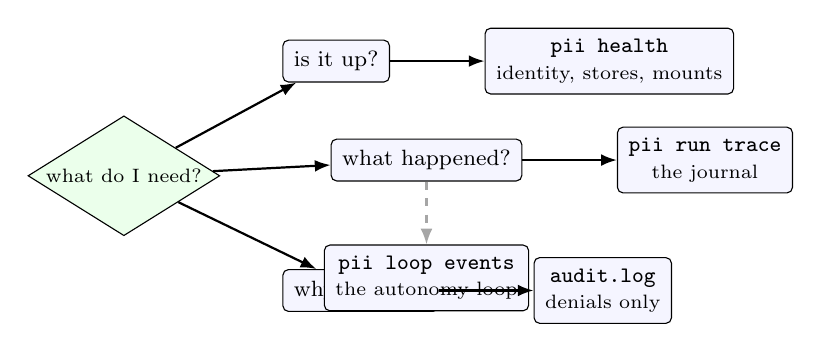
\begin{tikzpicture}[node distance=8mm and 12mm]
  \node[v] (q) {what do I need?};
  \node[b, above right=8mm and 14mm of q] (up) {is it up?};
  \node[b, right=14mm of q, yshift=2mm] (did) {what happened?};
  \node[b, below right=8mm and 14mm of q] (no) {why refused?};
  \node[b, right=of up] (health) {\texttt{pii health}\\\scriptsize identity, stores, mounts};
  \node[b, right=of did] (trace) {\texttt{pii run trace}\\\scriptsize the journal};
  \node[b, right=of no] (audit) {\texttt{audit.log}\\\scriptsize denials only};
  \node[b, below=of did] (loop) {\texttt{pii loop events}\\\scriptsize the autonomy loop};
  \draw[f] (q) -- (up);
  \draw[f] (q) -- (did);
  \draw[f] (q) -- (no);
  \draw[f] (up) -- (health);
  \draw[f] (did) -- (trace);
  \draw[f] (no) -- (audit);
  \draw[sf] (did) -- (loop);
\end{tikzpicture}}
\captionof{figure}{The entry point for each question. \texttt{pii health} is the right first command for all three, because it tells you whether the other surfaces can answer at all.}
\end{minipage}
\end{center}

\begin{center}
\begin{tabular}{@{}>{\raggedright\arraybackslash}p{0.20\textwidth}>{\raggedright\arraybackslash}p{0.28\textwidth}>{\raggedright\arraybackslash}p{0.42\textwidth}@{}}
  \toprule
  \textbf{Surface} & \textbf{Written by} & \textbf{Good for, and its limit} \\
  \midrule
  \texttt{pii health} & the daemon, on request & identity, config digest, stores, mounts,
    counters since deploy. It is a snapshot, not a history. \\
  the event log & the daemon, per event & everything the daemon decided. Off unless
    \texttt{-{}-log-file} or \texttt{[core].log\_file} is set. \\
  \texttt{audit.log} & the daemon, per denial & the security-relevant subset. Always on unless
    \texttt{-{}-audit off}. Never contains a kernel-level denial raised inside a child. \\
  the run journal & the engine, per run & what a run did, node by node, replayable. Grows with
    runs; retention applies. \\
  \bottomrule
\end{tabular}
\end{center}

\section{The anatomy of one event}

Every event is one JSON object on one line. The file sink adds a wall-clock stamp; the rest
of the object is the event itself.

\begin{center}
\begin{minipage}{\linewidth}
\centering
\resizebox{\linewidth}{!}{%
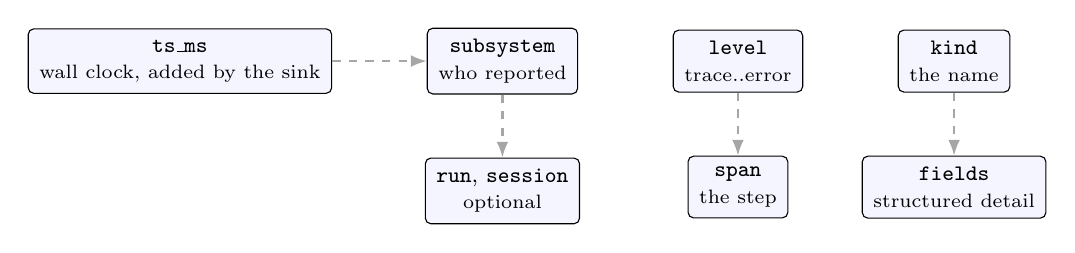
\begin{tikzpicture}[node distance=8mm and 12mm]
  \node[b] (ts) {\texttt{ts\_ms}\\\scriptsize wall clock, added by the sink};
  \node[b, right=of ts] (sub) {\texttt{subsystem}\\\scriptsize who reported};
  \node[b, right=of sub] (lvl) {\texttt{level}\\\scriptsize trace..error};
  \node[b, right=of lvl] (kind) {\texttt{kind}\\\scriptsize the name};
  \node[b, below=of kind] (fields) {\texttt{fields}\\\scriptsize structured detail};
  \node[b, below=of lvl] (span) {\texttt{span}\\\scriptsize the step};
  \node[b, below=of sub] (run) {\texttt{run}, \texttt{session}\\\scriptsize optional};
  \draw[sf] (ts) -- (sub);
  \draw[sf] (sub) -- (run);
  \draw[sf] (lvl) -- (span);
  \draw[sf] (kind) -- (fields);
\end{tikzpicture}}
\captionof{figure}{Six fields are always present (\texttt{ts\_ms}, \texttt{subsystem}, \texttt{level}, \texttt{kind}, \texttt{fields}, \texttt{span}); \texttt{run} and \texttt{session} appear only when the event belongs to one.}
\end{minipage}
\end{center}

The serialised form, with the run and session fields omitted because the event has neither:

\begin{lstlisting}[language=bash]
{"subsystem":"x","level":"info","kind":"k","fields":{"a":1},"span":null}
\end{lstlisting}

\texttt{level} is one of \texttt{trace}, \texttt{debug}, \texttt{info}, \texttt{warn},
\texttt{error}. In practice the daemon emits \texttt{info} for lifecycle, \texttt{warn} for
a refusal and \texttt{error} for a failure it could not prevent; \texttt{trace} and
\texttt{debug} exist in the type and are not the ones to grep for during an incident.

The two correlation fields are the reason a line can be trusted. \texttt{run} is the run id
and \texttt{session} the session id, so one \texttt{grep} answers \enquote{everything that
happened to this run} without matching a node name that three graphs share.

\section{The name registry}

Names are not string literals at call sites. Every event and every metric is a constant in one
file, and the file also holds an \texttt{ALL} array that a unit test checks for duplicates and
empty names. The count is exact and worth knowing, because it is the size of the vocabulary an
operator has to recognise:

\begin{center}
\begin{tabular}{@{}>{\raggedright\arraybackslash}p{0.30\textwidth}>{\raggedright\arraybackslash}p{0.16\textwidth}>{\raggedright\arraybackslash}p{0.44\textwidth}@{}}
  \toprule
  \textbf{Kind of name} & \textbf{Count} & \textbf{Where it is used} \\
  \midrule
  event names & 150 & the \texttt{kind} field of a log line, and the audit filter \\
  metric names & 40 & the series names \texttt{pii metrics} prints \\
  the \texttt{ALL} registry & 1 & the duplicate check, not emitted \\
  \midrule
  constants in the file & 191 & 150 + 40 + 1 \\
  \bottomrule
\end{tabular}
\end{center}

The 150 events fall into 38 subsystems. The largest are the ones an installation touches
every day: channels, learning, models, memory, runs.

\begin{center}
\begin{tabular}{@{}>{\raggedright\arraybackslash}p{0.16\textwidth}r@{\hspace{6mm}}>{\raggedright\arraybackslash}p{0.16\textwidth}r@{\hspace{6mm}}>{\raggedright\arraybackslash}p{0.16\textwidth}r@{}}
  \toprule
  \textbf{Subsystem} & \textbf{n} & \textbf{Subsystem} & \textbf{n} & \textbf{Subsystem} & \textbf{n} \\
  \midrule
  \texttt{channel} & 14 & \texttt{model} & 11 & \texttt{daemon} & 7 \\
  \texttt{learn} & 13 & \texttt{memory} & 10 & \texttt{mqtt} & 6 \\
  \texttt{run} & 10 & \texttt{coder} & 9 & \texttt{hal} & 6 \\
  \texttt{wasm} & 8 & \texttt{worker} & 5 & \texttt{trajectory} & 4 \\
  \texttt{proto} & 4 & \texttt{sop} & 4 & \texttt{graph} & 3 \\
  \texttt{net} & 3 & \texttt{cron} & 3 & \texttt{evolve} & 3 \\
  \texttt{timer} & 3 & \texttt{tools} & 2 & \texttt{queue} & 2 \\
  \texttt{tui} & 2 & \texttt{web} & 2 & \texttt{fetch} & 2 \\
  \texttt{effect} & 1 & \texttt{store} & 1 & \texttt{core} & 1 \\
  \texttt{health} & 1 & \texttt{observe} & 1 & \texttt{criteria} & 1 \\
  \texttt{skill} & 1 & \texttt{cli} & 1 & \texttt{lint} & 1 \\
  \texttt{cursor} & 1 & \texttt{mcp} & 1 & \texttt{node} & 1 \\
  \texttt{log} & 1 & \texttt{uds} & 1 & & \\
  \bottomrule
\end{tabular}
\end{center}

A few of the names are load-bearing enough to memorise, because they name the failures that
are otherwise silent:

\begin{center}\footnotesize
\begin{tabular}{@{}>{\raggedright\arraybackslash}p{0.34\textwidth}>{\raggedright\arraybackslash}p{0.56\textwidth}@{}}
  \toprule
  \textbf{Name} & \textbf{What it means when you see it} \\
  \midrule
  \texttt{graph.node.dead} & a node was marked dead; the run cannot proceed through it \\
  \texttt{graph.join.unsatisfiable} & a join can never be satisfied; the graph is wrong, not
    the run \\
  \texttt{observe.events.dropped} & the event pipeline dropped events; your log has a gap \\
  \texttt{core.cap.denied} & a capability the node did not hold was requested \\
  \texttt{store.persist.error} & a write to a store failed; the run's account is incomplete \\
  \texttt{model.provider.auth\_failed} & the key, not the model, is the problem \\
  \texttt{model.provider.rate\_limited} & the provider refused for quota; retrying now is waste \\
  \texttt{coder.env.refused} & a variable named in \texttt{env\_pass} was not passed \\
  \bottomrule
\end{tabular}
\end{center}

\section{Metrics}

\texttt{pii metrics} asks the daemon for its status payload and renders gauges and counters in
the text exposition format, one series per line, with labels in braces:

\begin{lstlisting}[language=bash]
pii_store_bytes{store="main"} 1048576
pii_runs 42
pii_run_latency_ms{outcome="succeeded",quantile="p95"} 132
\end{lstlisting}

It needs a running daemon: with none, it prints \enquote{no daemon answered} and exits 2. The
same numbers are in \texttt{pii health -{}-json}, which is the better choice when you want to
keep the payload for a record rather than read it.

\begin{center}
\begin{minipage}{\linewidth}
\centering
\resizebox{\linewidth}{!}{%
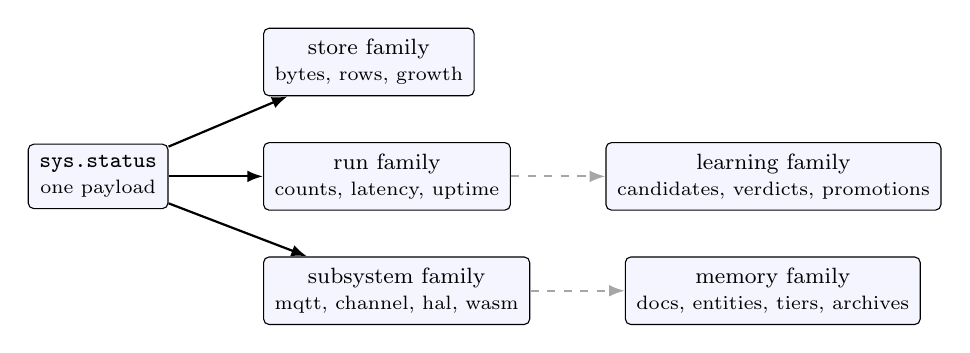
\begin{tikzpicture}[node distance=8mm and 12mm]
  \node[b] (sys) {\texttt{sys.status}\\\scriptsize one payload};
  \node[b, above right=6mm and 12mm of sys] (store) {store family\\\scriptsize bytes, rows, growth};
  \node[b, right=12mm of sys] (runs) {run family\\\scriptsize counts, latency, uptime};
  \node[b, below right=6mm and 12mm of sys] (sub) {subsystem family\\\scriptsize mqtt, channel, hal, wasm};
  \node[b, right=12mm of runs] (learn) {learning family\\\scriptsize candidates, verdicts, promotions};
  \node[b, right=12mm of sub] (mem) {memory family\\\scriptsize docs, entities, tiers, archives};
  \draw[f] (sys) -- (store);
  \draw[f] (sys) -- (runs);
  \draw[f] (sys) -- (sub);
  \draw[sf] (runs) -- (learn);
  \draw[sf] (sub) -- (mem);
\end{tikzpicture}}
\captionof{figure}{Six families, one payload. Every metric is derived from state the daemon already holds, so asking for metrics never changes what it is doing.}
\end{minipage}
\end{center}

The full set, with the label each series carries. \emph{Gauge} means a value that can go down;
\emph{counter} means one that only grows until the daemon restarts.

{\footnotesize
\begin{longtable}{@{}>{\raggedright\arraybackslash}p{0.33\textwidth}>{\raggedright\arraybackslash}p{0.08\textwidth}>{\raggedright\arraybackslash}p{0.47\textwidth}@{}}
  \toprule
  \textbf{Series} & \textbf{Type} & \textbf{Meaning} \\
  \midrule
  \endhead
  \texttt{pii\_runs} & gauge & runs in the main store \\
  \texttt{pii\_sessions} & gauge & sessions in the main store \\
  \texttt{pii\_approvals\_pending} & gauge & approvals awaiting a decision \\
  \texttt{pii\_journal\_events\_total} & counter & journal events ever appended \\
  \texttt{pii\_memory\_docs} & gauge & memory documents \\
  \texttt{pii\_cron\_entries} & gauge & configured cron entries \\
  \texttt{pii\_store\_bytes} & gauge, \texttt{store} & size of a store file in bytes \\
  \texttt{pii\_store\_format\_version} & gauge, \texttt{store} & persisted format version \\
  \texttt{pii\_rss\_bytes\_per\_run} & gauge & RSS growth per run over the recent window \\
  \texttt{pii\_process\_rss\_kb} & gauge & resident set size in KiB \\
  \texttt{pii\_store\_bytes\_per\_run} & gauge & main-store bytes divided by runs \\
  \texttt{pii\_run\_latency\_ms} & gauge, \texttt{outcome}, \texttt{quantile} & run latency,
    upper bucket bound \\
  \texttt{pii\_run\_latency\_count} & counter, \texttt{outcome} & runs in the histogram \\
  \texttt{pii\_uptime\_ms} & gauge & daemon uptime \\
  \texttt{pii\_mqtt\_received\_total} & counter & messages accepted from brokers \\
  \texttt{pii\_mqtt\_dropped\_total} & counter & messages dropped: queue full, not UTF-8 \\
  \texttt{pii\_mqtt\_published\_total} & counter & messages published \\
  \texttt{pii\_worker\_requests\_refused\_total} & counter & refusals around a drain or reload \\
  \texttt{pii\_channel\_posts\_total} & counter & messages a \texttt{post} node delivered \\
  \texttt{pii\_channel\_post\_refusals\_total} & counter & \texttt{post} calls refused or failed \\
  \texttt{pii\_quarantine\_refusals\_total} & counter & runs refused by a promotion quarantine \\
  \texttt{pii\_quarantine\_refusals\_recorded\_total} & counter & refusals whose deny reached the
    ledger; a gap to the line above is a finding \\
  \texttt{pii\_hal\_ops\_total} & counter, \texttt{kind} & HAL operations that succeeded \\
  \texttt{pii\_hal\_refusals\_total} & counter & HAL operations refused by claim or scope \\
  \texttt{pii\_wasm\_calls\_total} & counter, \texttt{outcome} & wasm calls by outcome \\
  \texttt{pii\_wasm\_refusals\_total} & counter & modules or calls refused before running \\
  \texttt{pii\_learn\_candidates} & gauge, \texttt{kind} & candidates from the last scan \\
  \texttt{pii\_learn\_refusals\_total} & counter & candidates refused for missing evidence \\
  \texttt{pii\_learn\_candidates\_proposed\_total} & counter & distinct candidates the unattended
    loop proposed \\
  \texttt{pii\_learn\_unattended\_runs\_total} & counter & unattended extract+verify passes \\
  \texttt{pii\_learn\_verdicts} & gauge, \texttt{verdict} & verdicts of the last verification \\
  \texttt{pii\_learn\_promotions} & gauge, \texttt{state} & promotions by state, plus
    \texttt{refused} \\
  \texttt{pii\_memory\_entities} & gauge & entities in the memory graph \\
  \texttt{pii\_memory\_relationships} & gauge & relationships in the memory graph \\
  \texttt{pii\_memory\_writes\_total} & counter, \texttt{kind} & writes that changed the graph \\
  \texttt{pii\_memory\_write\_refusals\_total} & counter, \texttt{reason} & memory writes refused \\
  \texttt{pii\_memory\_query\_refusals\_total} & counter, \texttt{reason} & memory queries refused \\
  \texttt{pii\_memory\_tier} & gauge, \texttt{tier} & records in each tier \\
  \texttt{pii\_memory\_tier\_changes\_total} & counter, \texttt{change} & transitions,
    \texttt{<from>\_to\_<to>} \\
  \texttt{pii\_memory\_archive\_ops\_total} & counter, \texttt{op} & archived, restored, refused \\
  \bottomrule
\end{longtable}
}

Two of these are instruments rather than descriptions. \texttt{pii\_store\_bytes\_per\_run} is
the growth rate as one number: a store that is not growing prints a small value, and a value
that climbs after every run names the subsystem to look at.
\texttt{pii\_quarantine\_refusals\_recorded\_total} exists to be compared with
\texttt{pii\_quarantine\_refusals\_total}: a refusal that did not reach the ledger is a defect
in the refusal path, not in the run.

\section{Health}

\texttt{pii health} prints the identity-bearing parts of the status payload, in a fixed order:

\begin{lstlisting}[language=bash]
# the shape of the output; values abbreviated
pii 0.2.0 (c05f3d1e4dd3, x86_64-unknown-linux-gnu)
client: c05f3d1e4dd3
config: /root/.pii/pii.toml sha256=9f2c...
stores:
  main: /run/user/0/pii/store.redb (1048576 bytes, format_version=1)
mounts:
  workspace [rw]: /projects/pi-improved  (workspace)
since_deploy:
  revision: c05f3d1e4dd3
  runs: 42
  starts: 3
  hard_deaths: 1
  runs_by_status.succeeded: 39
counts:
  runs: 42
\end{lstlisting}

Read it in three passes. \emph{Identity:} the binary's revision and this client's must match;
\texttt{config} names the file that is actually in force, with its digest. \emph{State:} the
stores and their format versions, then the mounts, which are the sandbox's answer to
\enquote{what may this daemon write}. \emph{History:} \texttt{since\_deploy} is the run of
numbers that survives a restart --- \texttt{starts} against \texttt{hard\_deaths} is the
crash record, and a \texttt{hard\_deaths} that grew since yesterday is the first thing to
explain.

\begin{center}
\begin{minipage}{\linewidth}
\centering
\resizebox{\linewidth}{!}{%
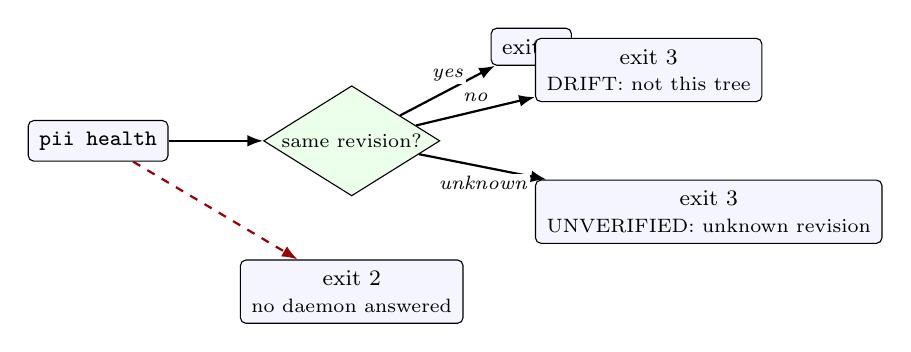
\begin{tikzpicture}[node distance=8mm and 12mm]
  \node[b] (h) {\texttt{pii health}};
  \node[v, right=of h] (rev) {same revision?};
  \node[b, above right=6mm and 12mm of rev] (ok) {exit 0};
  \node[b, right=of rev, yshift=9mm] (drift) {exit 3\\\scriptsize DRIFT: not this tree};
  \node[b, right=of rev, yshift=-9mm] (unk) {exit 3\\\scriptsize UNVERIFIED: unknown revision};
  \node[b, below=of rev] (down) {exit 2\\\scriptsize no daemon answered};
  \draw[f] (h) -- (rev);
  \draw[f] (rev) -- node[p, above=2pt, midway]{yes} (ok);
  \draw[f] (rev) -- node[p, above=2pt, midway]{no} (drift);
  \draw[f] (rev) -- node[p, below=2pt, midway]{unknown} (unk);
  \draw[bk] (h) -- (down);
\end{tikzpicture}}
\captionof{figure}{Three outcomes, two of them exit 3 for different reasons. \enquote{Unknown} is never treated as agreement: a build that cannot prove what it is has not proven it is current.}
\end{minipage}
\end{center}

The distinction between drift and unknown matters in an upgrade. Drift means the daemon is a
different, known binary: restart it with the new one. Unknown means one side has no revision
stamped, which is what a locally built binary without the build script looks like --- the
comparison cannot be made, and \texttt{pii health} will not pretend otherwise.

\section{The run journal}

The journal is the only account of what a run did, and it is append-only: every event is
written once, under \texttt{(run, seq)}. Seventeen event variants exist; the ones an operator
reads are these.

\begin{center}
\begin{tabular}{@{}>{\raggedright\arraybackslash}p{0.24\textwidth}>{\raggedright\arraybackslash}p{0.64\textwidth}@{}}
  \toprule
  \textbf{Journal event} & \textbf{What it records} \\
  \midrule
  \texttt{Started} & the graph name and a hash of the run input \\
  \texttt{TickStarted} & the batch of ready nodes drained in one scheduling tick, and its width \\
  \texttt{NodeStarted} & a node began, with its millisecond offset \\
  \texttt{NodeFinished} & the port it took, the value it produced, the value's hash, the
    duration \\
  \texttt{NodeFailed} & the error, whether it is retryable, and the attempt number \\
  \texttt{NodeProgress} & a heartbeat: elapsed time and child CPU. A wedged node shows elapsed
    growing while CPU stays flat. \\
  \texttt{NodeCancelled} & a node stopped because a person cancelled the run \\
  \texttt{NodeDead} & a node marked dead; the run cannot pass it \\
  \texttt{NodeInterrupted} & the node was cut short by a suspension or shutdown \\
  \texttt{Suspended}, \texttt{Resumed} & the run parked on a resume key, and continued \\
  \texttt{NodeRetried} & an explicit retry of one node \\
  \texttt{EffectStarted}, \texttt{EffectConfirmed} & a side effect began, and was confirmed \\
  \texttt{RunSpawned} & a child run was started, with its id \\
  \texttt{Finished} & the terminal outcome \\
  \bottomrule
\end{tabular}
\end{center}

\begin{center}
\begin{minipage}{\linewidth}
\centering
\resizebox{\linewidth}{!}{%
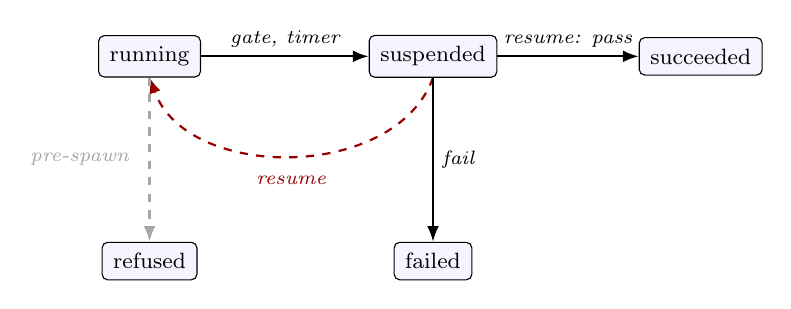
\begin{tikzpicture}[node distance=12mm and 16mm]
  \node[b] (run) at (0,0) {running};
  \node[b] (sus) at (3.6,0) {suspended};
  \node[b] (done) at (7.0,0) {succeeded};
  \node[b] (ref) at (0,-2.6) {refused};
  \node[b] (fail) at (3.6,-2.6) {failed};
  \draw[f] (run) -- node[p, above=2pt, midway]{gate, timer} (sus);
  \draw[f] (sus) -- node[p, above=2pt, midway]{resume: pass} (done);
  \draw[bk] (sus.south) to[out=250,in=290] node[p, below=6pt, midway]{resume} (run.south);
  \draw[f] (sus) -- node[p, right=2pt, midway]{fail} (fail);
  \draw[sf] (run) -- node[p, left=6pt, midway]{pre-spawn} (ref);
\end{tikzpicture}}
\captionof{figure}{Five statuses, and the one that is easy to miss. \texttt{Refused} means the agent call was refused before anything was spawned: it is not a failure of the work, and it is not in the \texttt{run ls -{}-status} vocabulary.}
\end{minipage}
\end{center}

That last point is a real limitation of the filter. \texttt{run ls -{}-status} accepts
\texttt{running}, \texttt{suspended}, \texttt{succeeded} and \texttt{failed}; the store's
fifth status, \texttt{refused}, cannot be named on the command line. A refused run therefore
appears in an unfiltered listing and disappears from every filtered one, which is exactly
when someone is looking for it.

\begin{lstlisting}[language=bash]
pii run ls                       # refused runs appear only here
pii run trace r000000000261 --reason implement
pii run trace r000000000261 --overlapped code,docs
pii run trace r000000000261 --terminal
\end{lstlisting}

\texttt{-{}-overlapped} is the query that answers a performance question without a profiler:
two nodes that were supposed to be sequential and were not show up as overlapped, and two
that were supposed to run together and never did show up as disjoint.

\section{The audit trail}

\texttt{audit.log} sits beside the store and receives only the security-relevant events. It is
rotated like the log, it is on by default, and it exists so that an operator can answer
\enquote{what was denied} without having enabled a full event log.

\begin{center}\footnotesize
\begin{tabular}{@{}>{\raggedright\arraybackslash}p{0.34\textwidth}>{\raggedright\arraybackslash}p{0.54\textwidth}@{}}
  \toprule
  \textbf{Kind in the trail} & \textbf{What it records} \\
  \midrule
  \texttt{core.cap.denied} & a capability the node did not hold \\
  \texttt{tools.deny\_list.hit} & a tool call matched the deny list \\
  \texttt{fetch.allowlist.denied} & a fetch to a host outside the allowlist \\
  \texttt{net.egress.denied} & egress outside \texttt{[net] grants} \\
  \texttt{daemon.sandbox.in\_force} & the profile, the exact grant, and whether confinement is
    applied \\
  \texttt{daemon.peer.refused} & a control peer refused at the socket \\
  \texttt{daemon.observer.detached} & the observer fan-out was switched off \\
  \texttt{daemon.audit.disabled} & the audit feed was switched off \\
  \bottomrule
\end{tabular}
\end{center}

A start writes \texttt{daemon.sandbox.in\_force} to the trail. It carries \texttt{profile},
\texttt{grant} and \texttt{enforced}, and it is the only place that states what the daemon was
actually confined to rather than what it was asked for.

One limit is structural and stated in the module that implements the filter: a denial raised
by the kernel inside a child process --- a raw redirect blocked by Landlock --- never passes
through pii and is therefore not in the trail. Only denials pii itself decides appear.

\begin{lstlisting}[language=bash]
grep daemon.sandbox.in_force /var/lib/pii/audit.log | tail -1
grep -c core.cap.denied /var/lib/pii/audit.log
grep net.egress.denied /var/lib/pii/audit.log | jq -r '.fields.host' | sort | uniq -c
\end{lstlisting}

With \texttt{-{}-audit off} the file is not empty: it records exactly one kind,
\texttt{daemon.audit.disabled}, so a trail that stops is distinguishable from a trail that was
never written.

\section{Incidents and the loop}

Two surfaces cover the unattended side, and neither needs a model.

\texttt{pii incidents scan -{}-source runtime -{}-log F} reads the daemon's own log and reports
each incident with its count, first and last seen, and \texttt{latency\_secs} against the
configured window --- the detection latency, which is the number that says whether the alert
arrived in time. Adding \texttt{-{}-ingest -{}-dir D} stores what it found;
\texttt{pii incidents show} reads one back. \texttt{pii incidents distance -{}-since} measures
the operator's own response time from recorded timestamps.

\texttt{pii loop emit} writes one NDJSON line per lifecycle step of an autonomy loop, and
\texttt{pii loop events} merges that file with the daemon log so the loop and the daemon read
as one timeline. The exit code carries information the text does not: \texttt{emit} keeps the
event locally and exits 3 when the daemon did not answer, appending \texttt{daemon=down} to
the detail. A loop that records 3s is a loop that was running while the daemon was not.

\section{Correlating a failure}

The order matters, because each step narrows the next.

\begin{center}
\begin{minipage}{\linewidth}
\centering
\resizebox{\linewidth}{!}{%
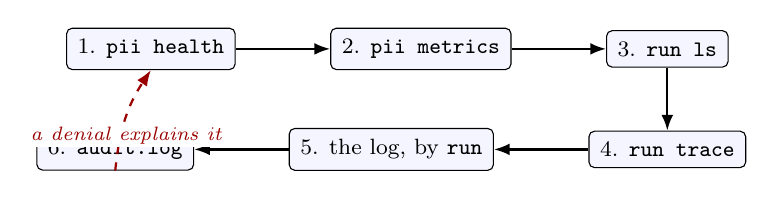
\begin{tikzpicture}[node distance=8mm and 12mm]
  \node[b] (one) {1. \texttt{pii health}};
  \node[b, right=of one] (two) {2. \texttt{pii metrics}};
  \node[b, right=of two] (three) {3. \texttt{run ls}};
  \node[b, below=of three] (four) {4. \texttt{run trace}};
  \node[b, left=of four] (five) {5. the log, by \texttt{run}};
  \node[b, left=of five] (six) {6. \texttt{audit.log}};
  \draw[f] (one) -- (two);
  \draw[f] (two) -- (three);
  \draw[f] (three) -- (four);
  \draw[f] (four) -- (five);
  \draw[f] (five) -- (six);
  \draw[bk] (six.south) to[bend left=14] node[p, below=2pt, midway]{a denial explains it} (one.south);
\end{tikzpicture}}
\captionof{figure}{Six steps from \enquote{something is wrong} to a cause. Steps 1 and 2 rule out the daemon; steps 3 to 5 locate the run and the node; step 6 explains a refusal that the run itself could not.}
\end{minipage}
\end{center}

\begin{longtable}{@{}>{\raggedright\arraybackslash}p{0.30\textwidth}>{\raggedright\arraybackslash}p{0.58\textwidth}@{}}
  \toprule
  \textbf{Symptom} & \textbf{First surface, and what to look for} \\
  \midrule
  \endhead
  every run fails in a second & the log, for \texttt{model.provider.auth\_failed} or
    \texttt{rate\_limited}; the metric set carries no model series, so this is an event
    question, not a metric one \\
  a run is \enquote{running} for hours & \texttt{run trace -{}-node-status}, then
    \texttt{NodeProgress}: elapsed growing with flat CPU is a wedged child \\
  the run stopped with no error & \texttt{run trace -{}-terminal}: a node left through a port
    with no edge, so nothing failed and nothing continued \\
  a write was refused & \texttt{audit.log}: \texttt{core.cap.denied} or
    \texttt{tools.deny\_list.hit}, never the run's own output \\
  the log has a gap & \texttt{observe.events.dropped}: the pipeline dropped events, so absence
    is not evidence \\
  the daemon restarted by itself & \texttt{pii health}: \texttt{hard\_deaths} in
    \texttt{since\_deploy}, and a log that ends on \texttt{daemon.started} with no
    \texttt{daemon.stopped} \\
  the metrics do not move & the daemon serving them is not the one running the work: compare
    \texttt{pii\_uptime\_ms} with the process you restarted \\
  \bottomrule
\end{longtable}

\begin{lstlisting}[language=bash]
pii health --json > /tmp/health.json
pii metrics | grep -E 'provider|store_bytes|latency'
pii run ls --status failed | jq -r '.[].run' | head
pii run trace "$RUN" --reason "$NODE"
grep "\"run\":\"$RUN\"" /var/log/pii/pii.log | jq -c 'select(.level!="info")'
grep -E 'cap.denied|egress.denied' /var/lib/pii/audit.log | tail -20
\end{lstlisting}
\chapter{The graph library}

\label{ch:graphs}

A graph is the unit of work in pii. An administrator needs three things from this chapter:
which graph to run for a job, what each graph will do to the machine, and how to read a run
that did not do what was expected. Every graph below was read from its file in
\texttt{graphs/}; where the generated page in \texttt{graphs/DOCS/} disagrees with the file,
the file wins and the disagreement is stated.

After the shape and the inventory, each graph gets one table with the same seven fields:
purpose, nodes, ports, entry and exit, capabilities, when to run, and how it fails.

\section{What a graph is, as an operator}

A graph has an \emph{entry} (where a run starts), named \emph{ports} on every node (how a step
reports its outcome), and --- if another graph may use it --- an \emph{exit}. It declares a
set of \emph{capabilities}, and a node may hold only what its graph holds. A port is not a
boolean: a judge has \texttt{ok}, \texttt{fail} and, in fail-expectation mode,
\texttt{unrunnable}; a queue \texttt{select} has four outcomes.

\begin{center}
\begin{minipage}{\linewidth}
\centering
\resizebox{\linewidth}{!}{%
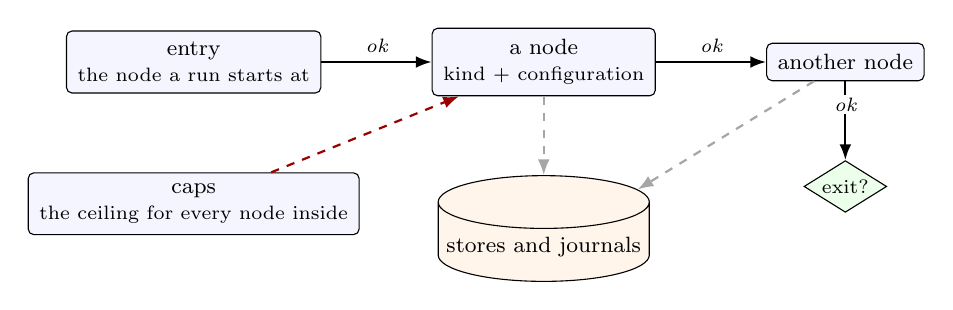
\begin{tikzpicture}[node distance=10mm and 14mm]
  \node[b] (entry) {entry\\\scriptsize the node a run starts at};
  \node[b, right=of entry] (work) {a node\\\scriptsize kind + configuration};
  \node[b, right=of work] (two) {another node};
  \node[s, below=of work] (store) {stores and journals};
  \node[b, below=of entry] (caps) {caps\\\scriptsize the ceiling for every node inside};
  \node[v, below=of two] (exit) {exit?};
  \draw[f] (entry) -- node[p, above=2pt, midway]{ok} (work);
  \draw[f] (work) -- node[p, above=2pt, midway]{ok} (two);
  \draw[sf] (work) -- (store);
  \draw[sf] (two) -- (store);
  \draw[bk] (caps) -- (work);
  \draw[f] (two) -- node[p, above=2pt, midway]{ok} (exit);
\end{tikzpicture}}
\captionof{figure}{The five things to look at in any graph file: where it starts, what each node does, which ports it can leave by, what the graph may touch, and whether it declares an exit.}
\end{minipage}
\end{center}

A graph without an exit is a \emph{run}, not a component: \texttt{docs} can be called
because it declares \texttt{exit = "docs"}, and \texttt{night} is callable because it declares
\texttt{exit = "report"}.

\section{The inventory}

Thirty-one files live under \texttt{graphs/}. Twenty-seven have a generated page in
\texttt{graphs/DOCS/}; the four that do not (\texttt{sdd}, \texttt{tdd}, \texttt{self-improve},
\texttt{doc-code}) are the most recently composed and the ones an operator is most likely to
run.

{\footnotesize
\begin{longtable}{@{}>{\raggedright\arraybackslash}p{0.25\textwidth}>{\raggedright\arraybackslash}p{0.07\textwidth}>{\raggedright\arraybackslash}p{0.16\textwidth}>{\raggedright\arraybackslash}p{0.28\textwidth}@{}}
  \toprule
  \textbf{Graph} & \textbf{Nodes} & \textbf{Entry $\to$ exit} & \textbf{Capabilities} \\
  \midrule
  \endhead
  \texttt{night} & 4 & \texttt{tick} $\to$ \texttt{report} & spawn, proc, post, fs\_read, fs\_write \\
  \texttt{sdd} & 8 & \texttt{contract} $\to$ \texttt{done} & spawn, proc, fs\_read, fs\_write \\
  \texttt{tdd} & 9 & \texttt{write\_test} $\to$ \texttt{green} & spawn, proc, fs\_read, fs\_write \\
  \texttt{queue} & 3 & \texttt{select} $\to$ \texttt{record} & spawn, proc, fs\_read, fs\_write \\
  \texttt{spec} & 7 & \texttt{code} $\to$ \texttt{done} & spawn, proc, fs\_read, fs\_write \\
  \texttt{docs} & 1 & \texttt{docs} $\to$ \texttt{docs} & spawn, proc \\
  \texttt{doc-code} & 8 & \texttt{inventory} $\to$ \texttt{done} & spawn, proc, fs\_read, fs\_write \\
  \texttt{self-improve} & 6 & \texttt{case} $\to$ \texttt{report} & spawn, proc, fs\_read, fs\_write \\
  \texttt{preflight} & 3 & \texttt{verify} $\to$ --- & proc \\
  \texttt{claude-probe} & 3 & \texttt{code} $\to$ --- & spawn, proc \\
  \texttt{coder-demo} & 3 & \texttt{code} $\to$ --- & spawn, proc \\
  \texttt{coder-podman} & 3 & \texttt{code} $\to$ --- & spawn, proc \\
  \texttt{coder-selffix} & 3 & \texttt{code} $\to$ --- & spawn, proc \\
  \texttt{code-index} & 4 & --- $\to$ --- & --- (does not load) \\
  \texttt{intervention-report} & 6 & --- $\to$ --- & --- (does not load) \\
  \texttt{digest-now} & 5 & \texttt{devices} $\to$ --- & memory\_read, post \\
  \texttt{discord-digest} & 6 & \texttt{tick} $\to$ --- & memory\_read, post \\
  \texttt{discord-triage} & 3 & \texttt{classify} $\to$ --- & post \\
  \texttt{podman-guard} & 2 & --- $\to$ --- & --- (fragment) \\
  \texttt{starter/assistant} & 4 & \texttt{agent} $\to$ --- & fs\_read, fs\_write, proc, net \\
  \texttt{starter/boss-watch} & 5 & \texttt{tick} $\to$ --- & proc \\
  \texttt{starter/consolidate} & 3 & \texttt{tick} $\to$ --- & --- \\
  \texttt{starter/crash} & 1 & \texttt{boom} $\to$ --- & --- \\
  \texttt{starter/failover} & 10 & \texttt{primary} $\to$ --- & fs\_read, fs\_write, proc \\
  \texttt{starter/heal-fix} & 11 & \texttt{probe} $\to$ --- & fs\_read, fs\_write, proc \\
  \texttt{starter/heal-watch} & 4 & \texttt{tick} $\to$ --- & proc \\
  \texttt{starter/react} & 3 & \texttt{agent} $\to$ --- & fs\_read, fs\_write, proc \\
  \texttt{starter/slow} & 2 & \texttt{wait} $\to$ --- & --- \\
  \texttt{starter/soak} & 1 & \texttt{step} $\to$ --- & --- \\
  \texttt{starter/soak\_cron} & 2 & \texttt{tick} $\to$ --- & --- \\
  \texttt{starter/verify-fix} & 5 & \texttt{fix} $\to$ --- & fs\_read, fs\_write, proc \\
  \bottomrule
\end{longtable}
}

Two files in that list do not load in this build, and that belongs at the top rather than in
a footnote. \texttt{code-index.toml} and
\texttt{intervention-report.toml} put their name in a \texttt{[graph]} table and express
their edges as \texttt{depends\_on} on each node; the loader reads a top-level \texttt{name},
an \texttt{entry}, and \texttt{[[edge]]} triples, so it refuses both with
\texttt{missing 'name'}. They are design records, not runnable graphs, and
\texttt{pii graph lint} says so in one line.

Three more files fail validation rather than loading: \texttt{tdd} and everything spliced from
it. Section~\ref{sec:lint-status} has the measured status of all thirty-one files.

The generated pages are not stale by accident: they describe the \emph{installed} copies.
\texttt{pii graph list} compares each installed file with the repository copy and prints the
verdict, and on the machine this chapter was written on four graphs were \texttt{DRIFT}
(\texttt{queue}, \texttt{spec}, \texttt{coder-selffix}, \texttt{discord-digest}). The installed
\texttt{queue.toml} was still the four-node \texttt{dispatch}/\texttt{judge} version dated
2026-11-03, while the repository held the three-node version that calls \texttt{spec}, dated
2026-11-04 --- which is why \texttt{DOCS/queue.md} lists four nodes.
\texttt{DOCS/claude-probe.md} records a budget of zero where the file says
\texttt{max\_budget\_usd = 0.30}. When a page and a file disagree, ask which file the daemon
loads: the installed one, and \texttt{graph list} is how you see it.

\section{The lint status of the library}

\label{sec:lint-status}

\texttt{pii graph lint} is the check that decides whether a file can run at all, so it was run
against every file. The result is not what the file list suggests.

\begin{center}\footnotesize
\begin{tabular}{@{}p{0.16\textwidth}p{0.10\textwidth}p{0.62\textwidth}@{}}
  \toprule
  \textbf{Exit} & \textbf{Files} & \textbf{What it means} \\
  \midrule
  0 & 26 & loads and validates; warnings only (V5: a declared port with no edge ---
    normal for a terminal node, and the thing to read for a node in the middle) \\
  3 & 3 & \texttt{tdd}, \texttt{sdd}, \texttt{night}: \texttt{V9: node '<n>' uses a
    multi-arm join with 1 inbound data edges}, once per single-armed \texttt{refuse} node \\
  2 & 2 & \texttt{code-index}, \texttt{intervention-report}: \texttt{invalid: missing 'name'} \\
  \bottomrule
\end{tabular}
\end{center}

The three V9 failures are one defect seen three times. Each of \texttt{tdd}'s refusal
terminals (\texttt{not-red}, \texttt{unrunnable}, \texttt{still-red}) declares
\texttt{join = "any"} and receives exactly one edge; the validator treats a multi-arm join
with one arm as a typo, so it refuses the graph. \texttt{sdd} inherits the failure because it
splices \texttt{tdd}, and \texttt{night} inherits it because it splices \texttt{sdd} --- which
is why the failure is reported with namespaced ids such as \texttt{sdd\_\_tdd\_\_not-red}.

The practical consequence is stark and belongs at the top of this chapter rather than in a
footnote: \emph{the TDD and SDD flows do not lint in this build, so they cannot start}. What
does run today is \texttt{queue}, \texttt{spec} and \texttt{docs} (the row lane),
\texttt{doc-code}, \texttt{self-improve}, \texttt{preflight} and the samples. An operator who
schedules \texttt{night} will see it refuse at load, with the V9 lines printed to stderr and
exit 3.

\begin{lstlisting}[language=bash]
pii graph lint graphs/tdd.toml     # 3 x V9, exit 3
pii graph lint graphs/sdd.toml     # the same nodes, namespaced tdd__not-red
pii graph lint graphs/night.toml   # the same nodes, namespaced sdd__tdd__not-red
pii graph lint graphs/queue.toml   # exit 0, warnings about record's unused ports
\end{lstlisting}

\section{How the pieces compose}

Only a few \texttt{call} nodes exist, and each one is a decision that a callee is the right
owner of a step.

\begin{center}
\begin{minipage}{\linewidth}
\centering
\resizebox{\linewidth}{!}{%
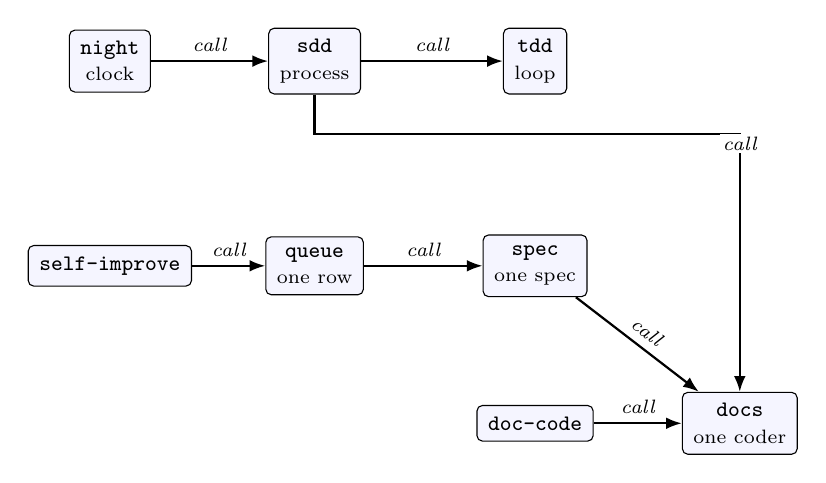
\begin{tikzpicture}[node distance=12mm and 14mm]
  \node[b] (night) at (-3.6,1.2) {\texttt{night}\\\scriptsize clock};
  \node[b] (sdd) at (-1.0,1.2) {\texttt{sdd}\\\scriptsize process};
  \node[b] (tdd) at (1.8,1.2) {\texttt{tdd}\\\scriptsize loop};
  \node[b] (self) at (-3.6,-1.4) {\texttt{self-improve}};
  \node[b] (queue) at (-1.0,-1.4) {\texttt{queue}\\\scriptsize one row};
  \node[b] (spec) at (1.8,-1.4) {\texttt{spec}\\\scriptsize one spec};
  \node[b] (docs) at (4.4,-3.4) {\texttt{docs}\\\scriptsize one coder};
  \node[b] (code) at (1.8,-3.4) {\texttt{doc-code}};
  \draw[f] (night) -- node[p, above=2pt, midway]{call} (sdd);
  \draw[f] (sdd) -- node[p, above=2pt, midway]{call} (tdd);
  \draw[f] (self) -- node[p, above=2pt, midway]{call} (queue);
  \draw[f] (queue) -- node[p, above=2pt, midway]{call} (spec);
  \draw[f] (spec) -- node[p, above=2pt, midway, sloped]{call} (docs);
  \draw[f] (code) -- node[p, above=2pt, midway]{call} (docs);
  \draw[f] (sdd.south) -- ++(0,-0.5) -| node[p, above=2pt, pos=0.55]{call} (docs.north);
\end{tikzpicture}}
\captionof{figure}{Every \texttt{call} in the library. Each arrow is pinned by sha256, so a change to the callee refuses to load until someone re-pins it deliberately.}
\end{minipage}
\end{center}

The pinned digest is what makes composition safe rather than convenient: \texttt{sdd} pins
\texttt{tdd} and \texttt{docs}, \texttt{queue} pins \texttt{spec}, and \texttt{night} pins
\texttt{sdd}. Edit \texttt{docs.toml} and every host that calls it refuses to load; that
refusal is the review gate.

\section{The operator flows}

\subsection*{\texttt{night} --- the clock}

\begin{center}
\begin{minipage}{\linewidth}
\centering
\resizebox{0.92\linewidth}{!}{%
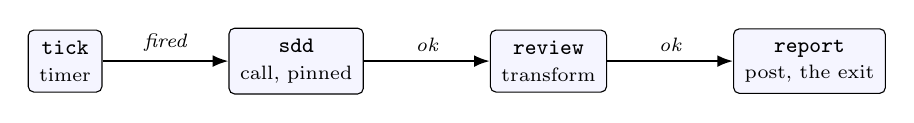
\begin{tikzpicture}[node distance=10mm and 16mm]
  \node[b] (tick) {\texttt{tick}\\\scriptsize timer};
  \node[b, right=of tick] (sdd) {\texttt{sdd}\\\scriptsize call, pinned};
  \node[b, right=of sdd] (review) {\texttt{review}\\\scriptsize transform};
  \node[b, right=of review] (report) {\texttt{report}\\\scriptsize post, the exit};
  \draw[f] (tick) -- node[p, above=2pt, midway]{fired} (sdd);
  \draw[f] (sdd) -- node[p, above=2pt, midway]{ok} (review);
  \draw[f] (review) -- node[p, above=2pt, midway]{ok} (report);
\end{tikzpicture}}
\captionof{figure}{\texttt{night} adds only two things to the work: time, and telling a human. Everything between is a call.}
\end{minipage}
\end{center}

\begin{center}\footnotesize
\begin{tabular}{@{}>{\raggedright\arraybackslash}p{0.15\textwidth}>{\raggedright\arraybackslash}p{0.75\textwidth}@{}}
  purpose & run the day's work on a clock and report it; it implements nothing itself \\
  nodes & \texttt{tick} timer; \texttt{sdd} call(\texttt{sdd}); \texttt{review} transform;
    \texttt{report} post \\
  ports & \texttt{tick.fired}, \texttt{sdd.ok}, \texttt{review.ok}; \texttt{report} is terminal \\
  entry/exit, caps & \texttt{tick} $\to$ \texttt{report}; \texttt{max\_wall\_ms = 7200000}; spawn, proc, post, fs\_read, fs\_write \\
  when & a host that should work unattended overnight; the run input needs
    \texttt{workdir} and \texttt{to} \\
  lint & exit 3: the spliced \texttt{tdd} refuse nodes fail V9, so the graph does not load
    in this build \\
  fails & a changed \texttt{sdd} refuses to load (pin); a refusal inside \texttt{sdd} has no
    edge here, so the night stops silently; a missing \texttt{to} fails at \texttt{report} \\
\end{tabular}
\end{center}

The silent stop is the one to watch for, and it is a property of the splice rather than of
\texttt{night}: \texttt{sdd}'s \texttt{unverified} and \texttt{refused} nodes are
\texttt{refuse} nodes, which declare no \texttt{ok} port, so a refused implementation never
returns a port the host can route. \texttt{queue} avoids this by wiring
\texttt{implement.unverified} and \texttt{implement.refused} by name; \texttt{night} does not
wire them, because until recently the callee had no such ports to name.

\subsection*{\texttt{queue} and \texttt{spec} --- one row, one implementation}

\begin{center}
\begin{minipage}{\linewidth}
\centering
\resizebox{\linewidth}{!}{%
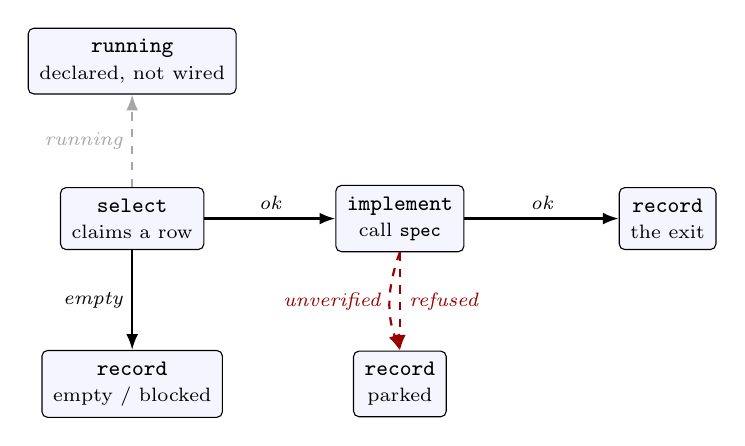
\begin{tikzpicture}[node distance=12mm and 16mm]
  \node[b] (select) at (0,0) {\texttt{select}\\\scriptsize claims a row};
  \node[b] (impl) at (3.4,0) {\texttt{implement}\\\scriptsize call \texttt{spec}};
  \node[b] (record) at (6.8,0) {\texttt{record}\\\scriptsize the exit};
  \node[b] (running) at (0,2) {\texttt{running}\\\scriptsize declared, not wired};
  \node[b] (park) at (3.4,-2.1) {\texttt{record}\\\scriptsize parked};
  \node[b] (none) at (0,-2.1) {\texttt{record}\\\scriptsize empty / blocked};
  \draw[f] (select) -- node[p, above=2pt, midway]{ok} (impl);
  \draw[f] (impl) -- node[p, above=2pt, midway]{ok} (record);
  \draw[bk] (impl) -- node[p, right=2pt, midway]{refused} (park);
  \draw[bk] (impl.south) to[out=250,in=110] node[p, left=2pt, midway]{unverified} (park.north);
  \draw[f] (select) -- node[p, left=2pt, midway]{empty} (none);
  \draw[sf] (select) -- node[p, left=2pt, midway]{running} (running);
\end{tikzpicture}}
\captionof{figure}{\texttt{queue} has three nodes: a claim, a call, a record. The grey port is declared by the node and has no edge, which is why a contested claim stops the run.}
\end{minipage}
\end{center}

\begin{center}\footnotesize
\begin{tabular}{@{}>{\raggedright\arraybackslash}p{0.15\textwidth}>{\raggedright\arraybackslash}p{0.75\textwidth}@{}}
  purpose & implement one queue row: claim it, call the spec graph with the row's spec, record
    the verdict \\
  nodes & \texttt{select} select; \texttt{implement} call(\texttt{spec}, pinned); \texttt{record} record \\
  ports & \texttt{select.ok}, \texttt{select.empty}, \texttt{select.blocked};
    \texttt{implement.ok}, \texttt{.unverified}, \texttt{.refused}; \texttt{record.ok} \\
  entry/exit, caps & \texttt{select} $\to$ \texttt{record}; \texttt{max\_wall\_ms = 6000000}; spawn, proc, fs\_read, fs\_write \\
  when & an operator or \texttt{night} has rows to work; run input carries \texttt{workdir}
    and \texttt{base} \\
  fails & a \texttt{running} claim (another run holds the row) has no edge, so the run ends
    without recording; \texttt{empty} and \texttt{blocked} reach \texttt{record} and write
    nothing; a refusal is recorded as \texttt{parked}, not as a failure \\
\end{tabular}
\end{center}

\texttt{record} writes to the queue store and to memory: the item's status becomes
\texttt{done} when the arriving value is the literal \texttt{done} or a verdict of
\texttt{passed}, and \texttt{parked} with the failing criterion otherwise. It also writes one
memory document per row, which is how a later digest knows what was implemented.

\subsection*{\texttt{tdd} --- a loop with three ways to prove nothing}

\begin{center}
\begin{minipage}{\linewidth}
\centering
\resizebox{\linewidth}{!}{%
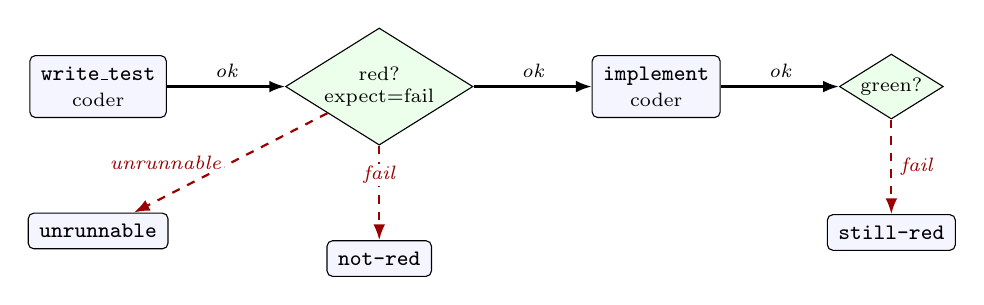
\begin{tikzpicture}[node distance=12mm and 15mm]
  \node[b] (write) {\texttt{write\_test}\\\scriptsize coder};
  \node[v, right=of write] (red) {red?\\\scriptsize expect=fail};
  \node[b, right=of red] (impl) {\texttt{implement}\\\scriptsize coder};
  \node[v, right=of impl] (green) {green?};
  \node[b, below=of green] (still) {\texttt{still-red}};
  \node[b, below=of red] (notred) {\texttt{not-red}};
  \node[b, below=of write] (unrun) {\texttt{unrunnable}};
  \draw[f] (write) -- node[p, above=2pt, midway]{ok} (red);
  \draw[f] (red) -- node[p, above=2pt, midway]{ok} (impl);
  \draw[f] (impl) -- node[p, above=2pt, midway]{ok} (green);
  \draw[bk] (red) -- node[p, above=2pt, midway]{fail} (notred);
  \draw[bk] (red) -- node[p, left=2pt, midway]{unrunnable} (unrun);
  \draw[bk] (green) -- node[p, right=2pt, midway]{fail} (still);
\end{tikzpicture}}
\captionof{figure}{The RED proof is the whole point: a test that passes before the code exists leaves by \texttt{not-red}, and a criterion that cannot run leaves by \texttt{unrunnable} rather than counting as a red.}
\end{minipage}
\end{center}

\begin{center}\footnotesize
\begin{tabular}{@{}>{\raggedright\arraybackslash}p{0.15\textwidth}>{\raggedright\arraybackslash}p{0.75\textwidth}@{}}
  purpose & one test-driven iteration: write the tests, prove them red, implement, prove them
    green \\
  nodes & \texttt{write\_test} coder; \texttt{red} judge(expect fail); \texttt{implement}
    coder; \texttt{green} judge; \texttt{done}; and four \texttt{refuse} terminals \\
  ports & \texttt{ok}/\texttt{err} on the coders; \texttt{ok}/\texttt{fail}/\texttt{unrunnable}
    on \texttt{red}; \texttt{ok}/\texttt{fail} on \texttt{green} \\
  entry/exit & \texttt{write\_test} $\to$ \texttt{green}; \texttt{max\_wall\_ms = 4200000};
    coders at \texttt{timeout\_ms = 1800000} \\
  caps & spawn, proc, fs\_read, fs\_write \\
  when & a spec whose exit criteria name behaviours; it is the loop \texttt{sdd} calls \\
  lint & exit 3: \texttt{not-red}, \texttt{unrunnable} and \texttt{still-red} each declare
    \texttt{join = "any"} with one inbound edge (V9), so the graph does not load \\
  fails & \texttt{not-red} (tests pass already), \texttt{unrunnable} (a criterion cannot
    run), \texttt{still-red} (the code did not make it pass), \texttt{refused} (the agent
    failed) \\
\end{tabular}
\end{center}

Only one of the four terminals (\texttt{still-red}) means the code was wrong.
\texttt{not-red} means the test was worthless --- a defect in the spec or in the test, not in
the implementation.

\subsection*{\texttt{sdd} --- the process around the loop}

\begin{center}\footnotesize
\begin{tabular}{@{}>{\raggedright\arraybackslash}p{0.15\textwidth}>{\raggedright\arraybackslash}p{0.75\textwidth}@{}}
  purpose & implement one spec under a contract: prove the criteria fail first, run
    \texttt{tdd}, verify, document, re-verify \\
  nodes & \texttt{contract} judge(expect fail); \texttt{tdd} call; \texttt{verify} judge;
    \texttt{docs} call; \texttt{reverify} judge; \texttt{done}; \texttt{unverified},
    \texttt{refused} \\
  ports & \texttt{contract.ok/fail/unrunnable}; \texttt{tdd.ok/fail}; \texttt{verify.ok/fail};
    \texttt{docs.ok/err}; \texttt{reverify.ok/fail} \\
  entry/exit & \texttt{contract} $\to$ \texttt{done}; needs \texttt{agent}, \texttt{model},
    \texttt{provider}, \texttt{spec}, \texttt{workdir}, \texttt{base}, \texttt{docs\_brief} \\
  caps & spawn, proc, fs\_read, fs\_write \\
  when & you have a spec and want the whole cycle, including documentation, in one run \\
  lint & exit 3: the spliced \texttt{tdd} nodes fail V9 under the \texttt{tdd\_\_} prefix \\
  fails & contract \texttt{fail} means the criteria already pass, which is a spec that proves
    nothing; docs that break the criteria end at \texttt{unverified}; a refusal is not
    returned to a host \\
\end{tabular}
\end{center}

\subsection*{\texttt{spec} --- one spec, by hand}

\begin{center}\footnotesize
\begin{tabular}{@{}>{\raggedright\arraybackslash}p{0.15\textwidth}>{\raggedright\arraybackslash}p{0.75\textwidth}@{}}
  purpose & implement one spec and document it, with three honest verdicts \\
  nodes & \texttt{code} coder; \texttt{verify} judge; \texttt{docs} call; \texttt{reverify}
    judge; \texttt{done}; \texttt{unverified}; \texttt{refused} \\
  ports & \texttt{code.ok/err}; \texttt{verify.ok/fail}; \texttt{docs.ok/err};
    \texttt{reverify.ok/fail} \\
  entry/exit & \texttt{code} $\to$ \texttt{done}; \texttt{max\_micro\_usd = 1000000},
    \texttt{max\_wall\_ms = 6000000} \\
  caps & spawn, proc, fs\_read, fs\_write \\
  when & you have a spec and want code plus docs without the TDD contract step \\
  fails & \texttt{unverified} is the honest middle: code exists and the criteria fail;
    \texttt{refused} means the coder or the docs call failed \\
\end{tabular}
\end{center}

\subsection*{\texttt{docs} and \texttt{doc-code} --- documentation, called and checked}

\begin{center}\footnotesize
\begin{tabular}{@{}>{\raggedright\arraybackslash}p{0.15\textwidth}>{\raggedright\arraybackslash}p{0.75\textwidth}@{}}
  purpose & write documentation for whatever brief the host passes; no inventory, no criteria,
    no opinion about truth \\
  nodes & \texttt{docs} coder (the entry and the exit) \\
  ports & \texttt{ok} on success; the coder's \texttt{err} otherwise \\
  entry/exit & \texttt{docs} $\to$ \texttt{docs}; needs \texttt{agent}, \texttt{model},
    \texttt{provider}, \texttt{spec}, \texttt{workdir}, \texttt{brief};
    \texttt{timeout\_ms = 1200000} \\
  caps & spawn, proc \\
  when & never directly: it is called by \texttt{spec}, \texttt{sdd} and \texttt{doc-code} \\
  fails & called without a \texttt{brief} it has nothing to write; it cannot tell whether the
    document is true, which is why \texttt{doc-code} exists \\
\end{tabular}
\end{center}

\begin{center}\footnotesize
\begin{tabular}{@{}>{\raggedright\arraybackslash}p{0.15\textwidth}>{\raggedright\arraybackslash}p{0.75\textwidth}@{}}
  purpose & document the code itself: list the modules with no \texttt{//!} header, write for
    them, then prove every path and symbol the document names exists \\
  nodes & \texttt{inventory} tool; \texttt{select} route; \texttt{nothing-to-do} transform;
    \texttt{write} call(\texttt{docs}); \texttt{verify} tool; \texttt{gate} route;
    \texttt{done}; \texttt{unverified} \\
  ports & \texttt{select.nothing-to-do/write}; \texttt{gate.pass/fail}; \texttt{ok}/\texttt{err}
    on the tools and the call \\
  entry/exit, caps & \texttt{inventory} $\to$ \texttt{done}; \texttt{max\_wall\_ms = 1800000}; spawn, proc, fs\_read, fs\_write \\
  when & a tree with undocumented modules; a documented tree ends at
    \texttt{nothing-to-do} and writes nothing \\
  fails & an inventory that cannot run, a docs call that fails, or a document naming a path
    that does not exist all end at \texttt{unverified} \\
\end{tabular}
\end{center}

\subsection*{\texttt{self-improve} --- a finding becomes work}

\begin{center}
\begin{minipage}{\linewidth}
\centering
\resizebox{\linewidth}{!}{%
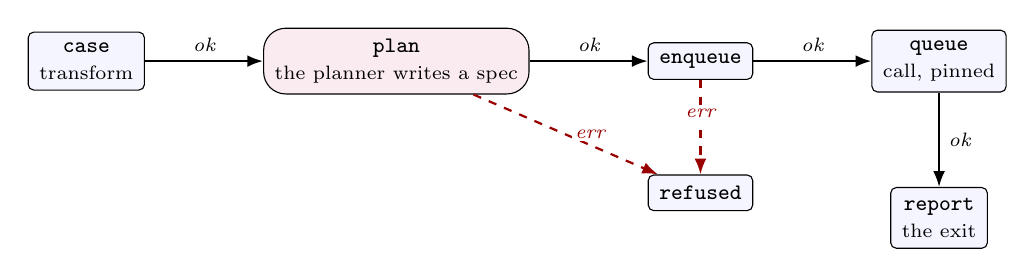
\begin{tikzpicture}[node distance=12mm and 15mm]
  \node[b] (case) {\texttt{case}\\\scriptsize transform};
  \node[m, right=of case] (plan) {\texttt{plan}\\\scriptsize the planner writes a spec};
  \node[b, right=of plan] (enq) {\texttt{enqueue}};
  \node[b, right=of enq] (queue) {\texttt{queue}\\\scriptsize call, pinned};
  \node[b, below=of queue] (report) {\texttt{report}\\\scriptsize the exit};
  \node[b, below=of enq] (refused) {\texttt{refused}};
  \draw[f] (case) -- node[p, above=2pt, midway]{ok} (plan);
  \draw[f] (plan) -- node[p, above=2pt, midway]{ok} (enq);
  \draw[f] (enq) -- node[p, above=2pt, midway]{ok} (queue);
  \draw[f] (queue) -- node[p, right=2pt, midway]{ok} (report);
  \draw[bk] (plan) -- node[p, right=2pt, midway]{err} (refused);
  \draw[bk] (enq) -- node[p, above=2pt, midway]{err} (refused);
\end{tikzpicture}}
\captionof{figure}{A finding becomes one spec, the spec becomes one row, and the queue implements it. The planner and the implementer are different models on purpose.}
\end{minipage}
\end{center}

\begin{center}\footnotesize
\begin{tabular}{@{}>{\raggedright\arraybackslash}p{0.15\textwidth}>{\raggedright\arraybackslash}p{0.75\textwidth}@{}}
  purpose & turn a finding into a spec, admit it to the queue, and run the row \\
  nodes & \texttt{case} transform; \texttt{plan} plan(model \texttt{glm-5.3});
    \texttt{enqueue}; \texttt{queue} call(pinned); \texttt{report} transform;
    \texttt{refused} transform \\
  ports & \texttt{ok}/\texttt{err} on \texttt{plan} and \texttt{enqueue};
    \texttt{queue.ok} only is wired \\
  entry/exit, caps & \texttt{case} $\to$ \texttt{report}; \texttt{max\_wall\_ms = 6300000}; spawn, proc, fs\_read, fs\_write \\
  when & you have a finding and no spec; the input carries \texttt{finding},
    \texttt{workdir}, \texttt{base} \\
  fails & a spec that fails the house shape is refused at \texttt{enqueue}; the queue's
    \texttt{unverified}/\texttt{refused} ports are not wired, so a failed implementation
    stops the run at the call; the queue claims the next pending row, which is the new one
    only when nothing older waits \\
\end{tabular}
\end{center}

\section{The coder samples}

These four exist to prove one thing each, and none of them is a production lane.

\begin{center}\footnotesize
\begin{tabular}{@{}>{\raggedright\arraybackslash}p{0.15\textwidth}>{\raggedright\arraybackslash}p{0.75\textwidth}@{}}
  purpose & probe a Claude login through pii in one hard-capped turn; the verdict is the exit
    code \\
  nodes & \texttt{code} coder(agent \texttt{claude}, model \texttt{haiku});
    \texttt{done}; \texttt{refused} \\
  ports & \texttt{ok} $\to$ \texttt{done}; \texttt{err} $\to$ \texttt{refused} \\
  entry/exit & \texttt{code} $\to$ ---; \texttt{max\_budget\_usd = 0.30},
    \texttt{timeout\_ms = 150000} \\
  caps & spawn, proc \\
  when & before trusting a lane that uses Claude; it costs one turn \\
  fails & a missing login file (the credential arrives through \texttt{HOME}, never the
    graph); the scratch workdir must exist; 150 seconds is the whole budget \\
\end{tabular}
\end{center}

\begin{center}\footnotesize
\begin{tabular}{@{}>{\raggedright\arraybackslash}p{0.15\textwidth}>{\raggedright\arraybackslash}p{0.75\textwidth}@{}}
  purpose & the smallest working coder: one coder node, one verdict \\
  nodes & \texttt{code} coder(agent \texttt{pi}, model \texttt{deepseek-v4-flash});
    \texttt{done}; \texttt{refused} \\
  ports & \texttt{code.ok/err} \\
  entry/exit & \texttt{code} $\to$ ---; \texttt{max\_wall\_ms = 2100000},
    \texttt{timeout\_ms = 1800000} \\
  caps & spawn, proc \\
  when & as a template for a new coder graph \\
  fails & the model id is dead: no provider serves \texttt{deepseek-v4-flash}, so the run
    dies at spawn; the workdir is a literal path, so it does not travel \\
\end{tabular}
\end{center}

\begin{center}\footnotesize
\begin{tabular}{@{}>{\raggedright\arraybackslash}p{0.15\textwidth}>{\raggedright\arraybackslash}p{0.75\textwidth}@{}}
  purpose & the same coder inside a container, with \texttt{/tmp} as its workdir \\
  nodes & \texttt{code} coder(agent \texttt{pi}, model \texttt{deepseek-v4-flash});
    \texttt{done}; \texttt{refused} \\
  ports & \texttt{code.ok/err} \\
  entry/exit, caps & \texttt{code} $\to$ ---; \texttt{max\_wall\_ms = 2100000};\newline caps: spawn, proc \\
  when & as a template for the podman lane; the fragment it was meant to attach cannot be
    woven into it \\
  fails & the same dead model id; a \texttt{/tmp} workdir outside the run's write scope is
    refused by the sandbox rather than silently ignored \\
\end{tabular}
\end{center}

\begin{center}\footnotesize
\begin{tabular}{@{}>{\raggedright\arraybackslash}p{0.15\textwidth}>{\raggedright\arraybackslash}p{0.75\textwidth}@{}}
  purpose & a coder that fixes its own spec, on the current model \\
  nodes & \texttt{code} coder(agent \texttt{pi}, model
    \texttt{deepseek-v4.1-flash:cloud}); \texttt{done}; \texttt{refused} \\
  ports & \texttt{code.ok/err} \\
  entry/exit, caps & \texttt{code} $\to$ ---; \texttt{max\_wall\_ms = 2100000};\newline caps: spawn, proc \\
  when & a self-fix lane that must run without a human writing the spec \\
  fails & it once declared \texttt{name = "coder-demo"} and collided with that graph in the
    installed directory; the name is now its own, and a collision is the failure to check
    after copying a graph \\
\end{tabular}
\end{center}

\section{The awareness graphs}

\begin{center}\footnotesize
\begin{tabular}{@{}>{\raggedright\arraybackslash}p{0.15\textwidth}>{\raggedright\arraybackslash}p{0.75\textwidth}@{}}
  purpose & build the digest on demand: two recalls and a post, with the timer removed \\
  nodes & \texttt{devices} recall; \texttt{lessons} recall; \texttt{digest} post;
    \texttt{refused\_devices}, \texttt{refused\_lessons} transforms \\
  ports & \texttt{ok}/\texttt{err} on both recalls \\
  entry/exit & \texttt{devices} $\to$ ---; caps memory\_read, post \\
  when & a person asks for the digest now; the scheduled version cannot answer, because its
    entry is a timer and a run of it reports \enquote{suspended, in\_ms $\approx$ N} \\
  fails & a recall that errors ends at its own refusal terminal; a missing
    \texttt{to} in the input fails at the post \\
\end{tabular}
\end{center}

\begin{center}\footnotesize
\begin{tabular}{@{}>{\raggedright\arraybackslash}p{0.15\textwidth}>{\raggedright\arraybackslash}p{0.75\textwidth}@{}}
  purpose & the scheduled digest: recall devices, recall lessons, post into a thread \\
  nodes & \texttt{tick} timer; \texttt{devices}; \texttt{lessons}; \texttt{digest} post; two
    refusal terminals \\
  ports & \texttt{tick.fired}; \texttt{ok}/\texttt{err} on the recalls \\
  entry/exit & \texttt{tick} $\to$ ---; caps memory\_read, post; \texttt{limit = 50} \\
  when & a channel wants a recurring digest; the input carries the thread id \\
  fails & asking it to run \enquote{now} suspends it by construction; a channel that is not
    configured fails at the post \\
\end{tabular}
\end{center}

\begin{center}\footnotesize
\begin{tabular}{@{}>{\raggedright\arraybackslash}p{0.15\textwidth}>{\raggedright\arraybackslash}p{0.75\textwidth}@{}}
  purpose & triage one inbound Discord message with rules and no model \\
  nodes & \texttt{classify}; \texttt{reply} post; \texttt{done} \\
  ports & \texttt{classify.ok} $\to$ \texttt{reply}; \texttt{reply.ok} $\to$ \texttt{done} \\
  entry/exit & \texttt{classify} $\to$ ---; caps post only \\
  when & a channel ingress starts it per message; input carries text, chat, user, channel \\
  fails & an unrecognised text is classified \texttt{chat}; a reply goes to
    \texttt{\$.input.chat}, so a message without a chat id cannot be answered \\
\end{tabular}
\end{center}

\begin{center}\footnotesize
\begin{tabular}{@{}>{\raggedright\arraybackslash}p{0.15\textwidth}>{\raggedright\arraybackslash}p{0.75\textwidth}@{}}
  purpose & \texttt{code-index}: index the repository into memory on a schedule.
    \texttt{intervention-report}: turn an intervention's events into a dated report, gate it,
    post it, remember it \\
  nodes & \texttt{code-index}: \texttt{start} timer, \texttt{index} worker, \texttt{gate},
    \texttt{record} memory. \texttt{intervention-report}: \texttt{start} timer,
    \texttt{evidence} memory, \texttt{write} worker, \texttt{check} gate, \texttt{post},
    \texttt{record} memory \\
  ports & none readable: both express edges as \texttt{depends\_on} node fields, which this
    loader does not read \\
  entry/exit, caps & none; both put \texttt{name} in a \texttt{[graph]} table, so neither loads;\newline caps: none declared \\
  when & never in this build: \texttt{pii graph lint} refuses both with
    \texttt{invalid: missing 'name'} (exit 2) \\
  fails & at load, before anything runs. \texttt{code-index}'s own header records why it is
    not ready: the index verb it needs was a script dependency the production rule forbids \\
\end{tabular}
\end{center}

\section{Preflight and the fragment}

\begin{center}\footnotesize
\begin{tabular}{@{}>{\raggedright\arraybackslash}p{0.15\textwidth}>{\raggedright\arraybackslash}p{0.75\textwidth}@{}}
  purpose & prove the exit criteria are runnable before any agent is spawned \\
  nodes & \texttt{verify} judge; \texttt{done}; \texttt{refuse} \\
  ports & \texttt{verify.ok} $\to$ \texttt{done}; \texttt{verify.fail} $\to$ \texttt{refuse} \\
  entry/exit & \texttt{verify} $\to$ ---; caps proc only; \texttt{max\_wall\_ms = 600000} \\
  when & the lane runs it through the daemon before the real run; the judge's sandbox is the
    real judge's, so a criterion that cannot write the scratch refuses here \\
  fails & a criterion that cannot run ends at \texttt{refuse}, having spent no agent and no
    model budget \\
\end{tabular}
\end{center}

\begin{center}\footnotesize
\begin{tabular}{@{}>{\raggedright\arraybackslash}p{0.15\textwidth}>{\raggedright\arraybackslash}p{0.75\textwidth}@{}}
  purpose & a blocking guard: refuse a run whose input asks for podman, pass every other run \\
  nodes & \texttt{check} route; \texttt{refuse} refuse \\
  ports & \texttt{check.refuse} $\to$ \texttt{refuse}; every other input falls through \\
  entry/exit, caps & none: it is a fragment, attached by name with a sha256 pin;\newline caps: none of its own; it inherits the host's \\
  when & attach it to a host at a pre surface (\texttt{run.start} or \texttt{node.before}),
    which is allowed because it may block \\
  fails & attaching it by name without a pin installs whatever the file says today; the
    weave refuses an unwoven attach rather than running the host without its guard \\
\end{tabular}
\end{center}

\section{The starter graphs}

Twelve samples under \texttt{graphs/starter/}: templates and test seams, not production
lanes. Two exist only to break something on purpose.

{\footnotesize
\begin{longtable}{@{}>{\raggedright\arraybackslash}p{0.15\textwidth}>{\raggedright\arraybackslash}p{0.25\textwidth}>{\raggedright\arraybackslash}p{0.20\textwidth}>{\raggedright\arraybackslash}p{0.30\textwidth}@{}}
  \toprule
  \textbf{Graph} & \textbf{Nodes and ports} & \textbf{Entry, caps} & \textbf{When, and how it fails} \\
  \midrule
  \endhead
  \texttt{assistant} & \texttt{agent}; \texttt{reply}; \texttt{fail\_err};
    \texttt{fail\_budget}. Ports \texttt{ok}, \texttt{err}, \texttt{budget} & \texttt{agent};
    fs\_read, fs\_write, proc, net & an assistant loop with a turn cap (4) and a wall of
    600000 ms. A budget exit is a separate terminal from an error. \\
  \texttt{boss-watch} & \texttt{tick}; \texttt{check} heal\_detect; \texttt{cyc};
    \texttt{escalate} gate; \texttt{done}. Ports \texttt{ok}, \texttt{flake},
    \texttt{inconclusive}, \texttt{detected} & \texttt{tick}; proc & watches a boss process
    every 30 minutes. A detected failure suspends at the gate until a human decides; there is
    no \texttt{fs\_write} anywhere in it. \\
  \texttt{consolidate} & \texttt{tick}; \texttt{run} memory; \texttt{done}. Port
    \texttt{fired}, \texttt{ok} & \texttt{tick}; none & a scheduled consolidation. It has no
    error edge, so a failing memory node ends the run rather than routing it. \\
  \texttt{crash} & \texttt{boom} debug\_crash. No ports & \texttt{boom}; none & deliberately
    crashes the daemon to exercise the panic hook. Never install it on a host you care about. \\
  \texttt{failover} & \texttt{primary}, \texttt{secondary} agents; two routes; retry and
    compress transforms; \texttt{exhausted}; \texttt{done} & \texttt{primary}; fs\_read,
    fs\_write, proc & a model-failover ladder. \texttt{compress} and \texttt{exhausted} are
    deliberate dead ends: retrying cannot fix a payload that is too large. \\
  \texttt{heal-fix} & \texttt{probe}; \texttt{route\_probe}; \texttt{unexpected\_ok};
    \texttt{fix} agent; \texttt{retest}; \texttt{route\_retest}; \texttt{retry};
    \texttt{summarize}; \texttt{record\_fixed}; \texttt{escalate}; \texttt{done} &
    \texttt{probe}; fs\_read, fs\_write, proc & localise, patch, validate, escalate, in a
    disposable worktree. The fix agent has file tools only, no shell; \texttt{bash} runs only
    in \texttt{tool} nodes. \\
  \texttt{heal-watch} & \texttt{tick}; \texttt{check} heal\_detect; \texttt{escalate} gate;
    \texttt{done}. Ports \texttt{ok}, \texttt{flake}, \texttt{detected} & \texttt{tick};
    proc & runs the quality gate every 30 minutes, writes one ledger row for a reproducible
    failure, and suspends for acknowledgement. Read-only detection. \\
  \texttt{react} & \texttt{agent}; \texttt{done}; \texttt{fail} & \texttt{agent}; fs\_read,
    fs\_write, proc & react to one signal with 24 turns and compaction at 24k tokens. Both
    \texttt{err} and \texttt{budget} end at \texttt{fail}. \\
  \texttt{slow} & \texttt{wait} timer; \texttt{done} & \texttt{wait}; none & a 30-second wait,
    used to have a run in flight at SIGTERM. Not a workload. \\
  \texttt{soak} & \texttt{step} transform & \texttt{step}; none & one soak step, bounded to
    100 steps and 30 seconds. The harness runs many of them. \\
  \texttt{soak\_cron} & \texttt{tick}; \texttt{done} & \texttt{tick}; none & the same soak on
    a timer, bounded to 600000 ms. \\
  \texttt{verify-fix} & \texttt{fix} agent; \texttt{test} tool; \texttt{gate} route;
    \texttt{retry}; \texttt{done}. Ports \texttt{pass}, \texttt{fail} & \texttt{fix};
    fs\_read, fs\_write, proc & fix then verify, looping at most 3 times. A \texttt{fail}
    that keeps failing is a run that ends at the budget, not at a verdict. \\
  \bottomrule
\end{longtable}
}

\section{What the graphs can do to the machine}

The ladder is checked at load time: this is the set of refusals an author will meet.

\begin{longtable}{@{}>{\raggedright\arraybackslash}p{0.18\textwidth}>{\raggedright\arraybackslash}p{0.62\textwidth}@{}}
  \toprule
  \textbf{Capability} & \textbf{What it allows, and the refusal when it is missing} \\
  \midrule
  \endhead
  \texttt{fs\_read} & read the working tree \\
  \texttt{fs\_write} & modify the working tree. A coder without it stops and reports that no
    write tool is available; measured 2026-11-03, it did not degrade silently. \\
  \texttt{proc} & run a command. This is what lets a judge execute exit criteria, and what a
    \texttt{judge} node requires. \\
  \texttt{spawn} & start an agent process; every model call needs it \\
  \texttt{post} & send a message to a human; \texttt{night} and the report graphs hold it \\
  \texttt{memory\_read} & read the memory store; the digest graphs hold it \\
  \texttt{net} & reach the network under \texttt{[net] grants}; only the assistant sample
    holds it \\
  \bottomrule
\end{longtable}

Two refusals are worth being able to read at sight. \texttt{graph.call.widen} means a call
needs a capability its host does not hold --- the fix is in the host's \texttt{caps}, not in
the callee. And the lint code \texttt{V2} means a node needs a capability the graph does not
declare; the message names both the node and the capability, and it is the most common error
in a new graph.

\section{Reading a graph's failure}

A run that ends \emph{without} reaching a terminal node has not failed loudly: it took a port
with no edge, or it was spliced into a host that does not wire its refusals. The trace answers
that in one query --- \texttt{-{}-terminal} names where it stopped, \texttt{-{}-reason} why.

\begin{lstlisting}[language=bash]
pii graph lint graphs/night.toml        # V-codes, pins, caps before anything runs
pii graph list                          # installed vs repo: DRIFT is the interesting column
pii graph explain queue                 # nodes and ports in execution order
pii run start queue --input '{"workdir":"/projects/pi-improved","base":"<40-hex>"}'
pii run trace "$RUN" --terminal         # where it stopped
pii run trace "$RUN" --reason implement # why that node ended there
\end{lstlisting}


\chapter{Memory}

\label{ch:memory}

Everything else in this manual is about work: runs, rows, graphs, gates. This chapter is about
what survives the work — what pii remembers after a run ends, how it is found again, why some of
it fades, and what an operator should check when memory looks wrong. Scattered in earlier
chapters you will have seen memory mentioned next to the stores; that was a reference. This is the
chapter.

The short version, before the detail: \textbf{pii does not remember conversations. It remembers
documents.} A document is a piece of text with a layer, a kind, a set of concepts, and an id
derived from its own content. Nothing is remembered by being said; something is remembered by
being written, and writing the same text twice is the same document.

\section{The four things a document carries}

\begin{center}
\resizebox{\linewidth}{!}{
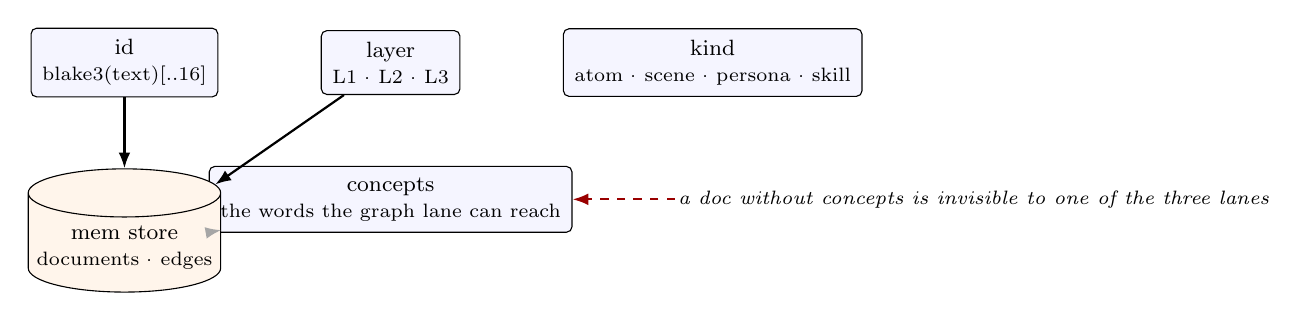
\begin{tikzpicture}[node distance=9mm and 13mm]
  \node[b] (id) {id\\\scriptsize blake3(text)[..16]};
  \node[b, right=of id] (layer) {layer\\\scriptsize L1 · L2 · L3};
  \node[b, right=of layer] (kind) {kind\\\scriptsize atom · scene · persona · skill};
  \node[b, below=of layer] (concepts) {concepts\\\scriptsize the words the graph lane can reach};
  \node[s, below=of id] (store) {mem store\\\scriptsize documents · edges};
  \node[p, right=of concepts] (note) {a doc without concepts is invisible to one of the three lanes};
  \draw[f] (id) -- (store);
  \draw[f] (layer) -- (store);
  \draw[sf] (concepts) -- (store);
  \draw[bk] (note) -- (concepts);
\end{tikzpicture}}
\captionof{figure}{The four fields that matter operationally. The id is derived, not assigned: two puts of the same text produce one document.}
\end{center}

Because the id is the hash of the text, \texttt{pii memory put} is \emph{idempotent}: writing the
same sentence twice does not create two memories, it rewrites one. That is also why editing a
memory means writing a new document — the text changed, so the id changed — and why a correction
appears as a new document rather than a modification of the old one.

\section{The three layers, and what each is for}

\begin{center}
\resizebox{\linewidth}{!}{
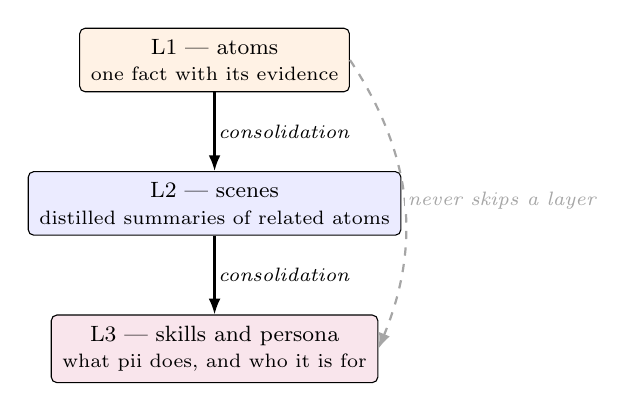
\begin{tikzpicture}[node distance=10mm and 8mm]
  \node[b, fill=orange!10, minimum width=3.4cm] (l1) {L1 — atoms\\\scriptsize one fact with its evidence};
  \node[b, fill=blue!8, below=of l1, minimum width=3.4cm] (l2) {L2 — scenes\\\scriptsize distilled summaries of related atoms};
  \node[b, fill=purple!10, below=of l2, minimum width=3.4cm] (l3) {L3 — skills and persona\\\scriptsize what pii does, and who it is for};
  \draw[f] (l1) -- node[p,right]{consolidation} (l2);
  \draw[f] (l2) -- node[p,right]{consolidation} (l3);
  \draw[sf] (l1.east) to[bend left=28] node[p,right]{never skips a layer} (l3.east);
\end{tikzpicture}}
\captionof{figure}{Consolidation moves upward and never backward. An atom is not a scene that lost detail; a scene is a set of atoms that agreed.}
\end{center}

The layers are not storage tiers — they are kinds of claim. An \textbf{atom} is one fact with
evidence: a single observation it would be wrong to generalise from. A \textbf{scene} is a
distillation of several atoms that share concepts: it says what the atoms together mean. \textbf{L3}
holds skills --- procedures pii can follow --- and the persona document, which is the one kind that
never decays.

Two consequences an operator should hold on to. First, a scene is derived: if you delete every
atom behind it, the scene remains but its evidence is gone, which is a reason to archive rather
than delete. Second, \texttt{same\_layer\_only} is on: consolidation will not merge an atom into
a scene, so a half-finished idea stays an atom until it earns its way up.

\section{How a memory is found: three lanes, one ranked list}

A search does not consult one index. Three independent lanes each produce candidates, and their
rankings are fused.

\begin{center}
\resizebox{\linewidth}{!}{
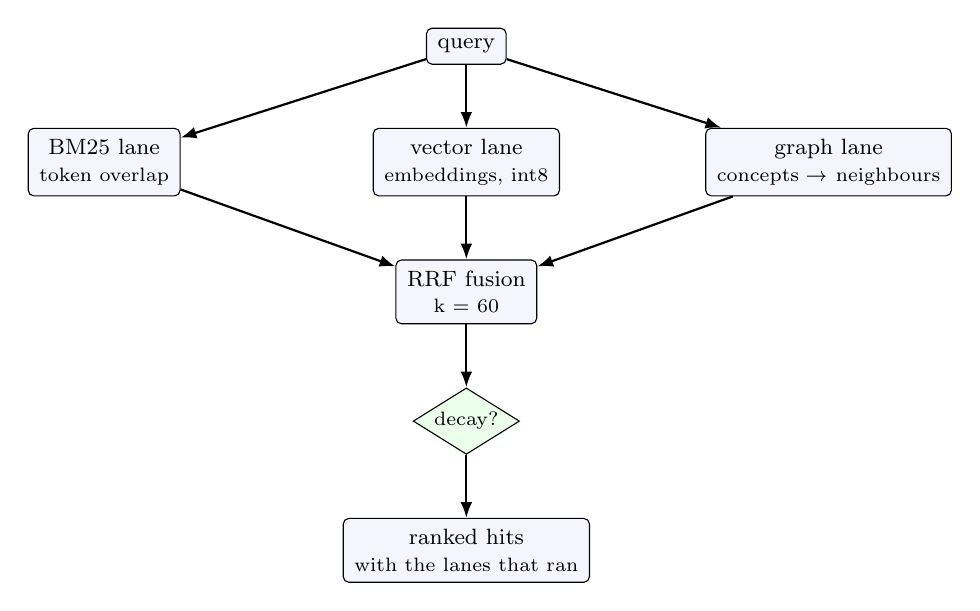
\begin{tikzpicture}[node distance=8mm and 11mm]
  \node[b] (q) {query};
  \node[b, below=of q, xshift=-4.6cm] (bm) {BM25 lane\\\scriptsize token overlap};
  \node[b, below=of q] (vec) {vector lane\\\scriptsize embeddings, int8};
  \node[b, below=of q, xshift=4.6cm] (gr) {graph lane\\\scriptsize concepts → neighbours};
  \node[b, below=of vec] (rrf) {RRF fusion\\\scriptsize k = 60};
  \node[v, below=of rrf] (decay) {decay?};
  \node[b, below=of decay] (ranked) {ranked hits\\\scriptsize with the lanes that ran};
  \draw[f] (q) -- (bm); \draw[f] (q) -- (vec); \draw[f] (q) -- (gr);
  \draw[f] (bm) -- (rrf); \draw[f] (vec) -- (rrf); \draw[f] (gr) -- (rrf);
  \draw[f] (rrf) -- (decay); \draw[f] (decay) -- (ranked);
\end{tikzpicture}}
\captionof{figure}{Fusion by rank, not by score. Reciprocal-rank fusion is used because the three lanes produce scores on incomparable scales — BM25 counts terms, cosine sits in $[-1,1]$, the graph lane counts hops.}
\end{center}

\textbf{Reciprocal-rank fusion} with $k = 60$ combines them: each lane contributes
$1/(k + \text{rank})$ per hit, and the sums decide the order. The practical effect is that a
document ranked first by one lane beats a document ranked fifth by all three, which is the
behaviour you want when one lane is much more confident than the rest.

Then decay is applied per kind, and here is the first thing that surprises operators:

\begin{center}
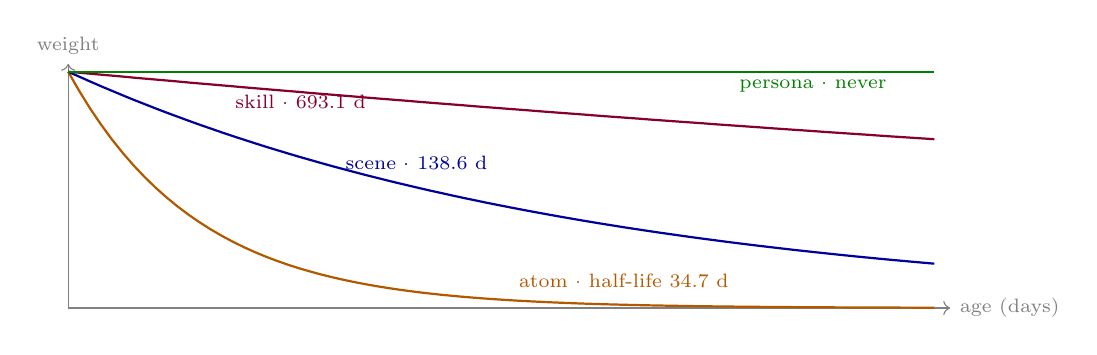
\begin{tikzpicture}[x=1cm, y=1cm]
  \draw[->, gray] (0,0) -- (11.2,0) node[right, font=\scriptsize] {age (days)};
  \draw[->, gray] (0,0) -- (0,3.1) node[above, font=\scriptsize] {weight};
  \draw[thick, orange!70!black] plot[domain=0:11, samples=80] (\x, {3*exp(-0.02*\x*30.4)});
  \draw[thick, blue!60!black]  plot[domain=0:11, samples=80] (\x, {3*exp(-0.005*\x*30.4)});
  \draw[thick, purple!70!black] plot[domain=0:11, samples=80] (\x, {3*exp(-0.001*\x*30.4)});
  \draw[thick, green!50!black] (0,3) -- (11,3);
  \node[font=\scriptsize, orange!70!black, right] at (5.6,0.35) {atom · half-life 34.7 d};
  \node[font=\scriptsize, blue!60!black, right] at (3.4,1.85) {scene · 138.6 d};
  \node[font=\scriptsize, purple!70!black, right] at (2.0,2.62) {skill · 693.1 d};
  \node[font=\scriptsize, green!50!black, right] at (8.4,2.82) {persona · never};
\end{tikzpicture}
\captionof{figure}{Decay is exponential, $\mathrm{score}\times e^{-\lambda\,\text{age}}$, with $\lambda$ fixed per kind. The half-lives are computed from the constants in the crate: 0.693/0.02, 0.693/0.005, 0.693/0.001.}
\end{center}

An atom written a month ago carries roughly half the weight of one written today; a skill written
two years ago still carries most of its weight. Decay reorders results, it does not delete
anything --- deletion is retention's job, and it is a separate mechanism (chapter~4).

\section{The graph lane, and why it often contributes nothing}

This is the intricacy most worth knowing, because it produces the most confusing symptom: a search
that returns obviously-related documents from BM25 and from vectors, while the graph lane appears
in the response and adds nothing.

The graph lane fires only when \emph{a query token is already a concept head present in the edge
table} --- that is, when some earlier document was written with that word in its concept list.
Free-text queries against documents stored without explicit concepts produce no query concepts at
all, so the lane contributes nothing.

\begin{center}
\resizebox{\linewidth}{!}{
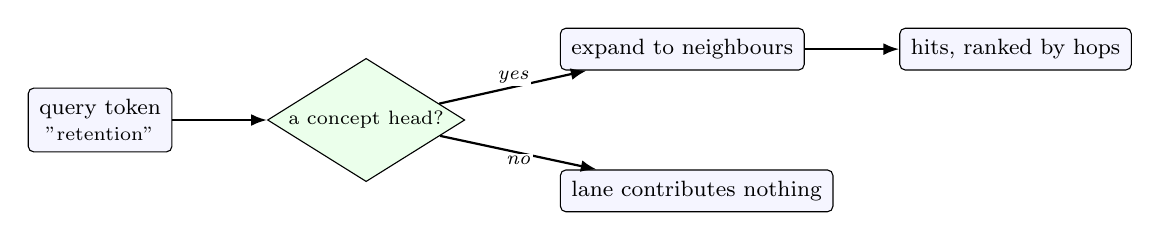
\begin{tikzpicture}[node distance=8mm and 12mm]
  \node[b] (query) {query token\\\scriptsize "retention"};
  \node[v, right=of query] (isconcept) {a concept head?};
  \node[b, right=of isconcept, yshift=9mm] (expand) {expand to neighbours};
  \node[b, right=of isconcept, yshift=-9mm] (nothing) {lane contributes nothing};
  \node[b, right=of expand] (hits) {hits, ranked by hops};
  \draw[f] (query) -- (isconcept);
  \draw[f] (isconcept) -- node[p,above]{yes} (expand);
  \draw[f] (isconcept) -- node[p,below]{no} (nothing);
  \draw[f] (expand) -- (hits);
\end{tikzpicture}}
\captionof{figure}{The lane reports that it RAN either way. ``Ran'' is not ``hit'' — the response lists the lanes that were consulted, not the lanes that found something.}
\end{center}

The operational reading: if the graph lane never contributes on your store, your documents were
written without concepts. \texttt{pii memory put} takes the text; the concept list is what makes a
document reachable by association. Writing facts through the fact path records concepts, and that
is how a store becomes navigable rather than merely searchable.

\section{Consolidation: when many atoms become one scene}

Consolidation is the process that turns atoms into a scene. It is deliberately conservative, and
each of its limits is worth knowing because each one explains a scene that never appeared.

\begin{longtable}{@{}p{0.34\textwidth}p{0.20\textwidth}p{0.36\textwidth}@{}}
  \toprule
  \textbf{Rule} & \textbf{Value} & \textbf{What it means to an operator} \\
  \midrule
  \endhead
  shared concepts & at least 2 & a single shared word is never enough to merge \\
  concept Jaccard & at least 0.15 & the two documents must be about mostly the same thing \\
  negation window & 8 tokens & a ``not'' near a shared concept vetoes the merge \\
  candidate cap & 200 & generation stops at 200 and says so in the report \\
  same layer only & on & an atom is never merged into a scene \\
  archive after & configured days & documents past their last use are archived, not deleted \\
  \bottomrule
\end{longtable}

The negation window is the one that saves you: ``the disk floor is 12\,GB'' and ``the disk floor is
not 12\,GB'' share every concept, and would otherwise consolidate into a scene that asserts both.

\section{The commands, and what each one touches}

\begin{longtable}{@{}p{0.26\textwidth}p{0.40\textwidth}p{0.26\textwidth}@{}}
  \toprule
  \textbf{Command} & \textbf{What it does} & \textbf{Reads / writes} \\
  \midrule
  \endhead
  \texttt{memory search} & fused search over the three lanes, returns hits and the lanes that ran & reads documents and edges \\
  \texttt{memory put} & writes a document; the id is the content hash, so a repeat is a no-op & writes one document \\
  \texttt{memory learn} & records an outcome as a document & writes one document \\
  \texttt{memory tiers} & what sits in L1, L2 and L3 & reads only \\
  \texttt{memory entity} & creates or reads an entity in the entity graph & writes entities \\
  \texttt{memory link} & creates an edge between entities & writes edges \\
  \texttt{memory neighbours} & the entities adjacent to one entity & reads edges \\
  \texttt{memory consolidate} & generates candidate merges under the rules above & writes scenes, archives \\
  \texttt{memory compact} & removes superseded versions of a document & writes \\
  \texttt{memory show} & one document, in full, with its metadata & reads \\
  \texttt{memory archive} / \texttt{restore} & takes a document out of search, or puts it back & writes \\
  \bottomrule
\end{longtable}

Most of these go through the daemon, because the daemon is the only writer. If you are told
\texttt{uds.connect.failed}, the daemon is down --- that is a supervision problem (chapter~2), not
a memory problem, and it is worth saying plainly because the error names a socket rather than the
cause.

\section{What goes wrong, in the order you will meet it}

\begin{longtable}{@{}p{0.30\textwidth}p{0.34\textwidth}p{0.28\textwidth}@{}}
  \toprule
  \textbf{Symptom} & \textbf{Cause} & \textbf{What to do} \\
  \midrule
  \endhead
  results are stale but present & decay, not deletion & search again with a recency bias, or re-put the fact \\
  a fact is gone & retention swept it, or it was archived & \texttt{memory show} the id; restore from backup if needed \\
  the graph lane never contributes & documents were written without concepts & write facts through the fact path \\
  the vector lane is skipped & no embedder configured, or zero dimensions & the response marks itself degraded; BM25 and the graph still answer \\
  two documents say the same thing & the text differed by a character & the ids differ by design; consolidate or archive \\
  a scene asserts something odd & merged atoms that disagreed & the negation window covers only 8 tokens; tighten the concepts \\
  search is slow & a large store with no compact & run \texttt{memory compact}, then measure again \\
  \bottomrule
\end{longtable}

\section{How memory is bounded}

Memory is bounded in four independent ways, and an administrator should know which one is doing
the work on their host:

\begin{center}
\resizebox{\linewidth}{!}{
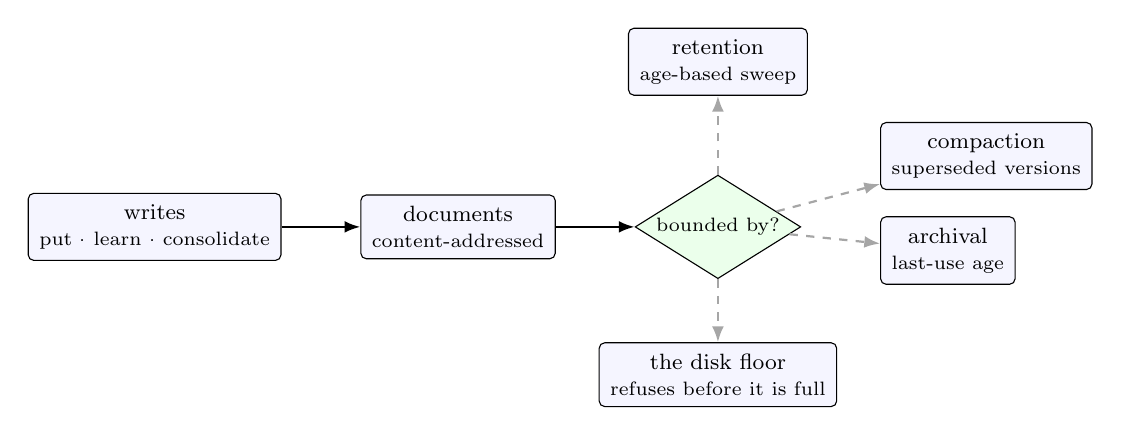
\begin{tikzpicture}[node distance=8mm and 10mm]
  \node[b] (write) {writes\\\scriptsize put · learn · consolidate};
  \node[b, right=of write] (docs) {documents\\\scriptsize content-addressed};
  \node[v, right=of docs] (bound) {bounded by?};
  \node[b, above=of bound, yshift=2mm] (ret) {retention\\\scriptsize age-based sweep};
  \node[b, right=of bound, yshift=9mm] (comp) {compaction\\\scriptsize superseded versions};
  \node[b, right=of bound, yshift=-3mm] (arch) {archival\\\scriptsize last-use age};
  \node[b, below=of bound] (disk) {the disk floor\\\scriptsize refuses before it is full};
  \draw[f] (write) -- (docs); \draw[f] (docs) -- (bound);
  \draw[sf] (bound) -- (ret); \draw[sf] (bound) -- (comp);
  \draw[sf] (bound) -- (arch); \draw[sf] (bound) -- (disk);
\end{tikzpicture}}
\captionof{figure}{Four bounds, four mechanisms, four different failure modes. ``Memory is full'' is never one thing; the question is which bound fired.}
\end{center}

The order to investigate: \texttt{pii store df} first (how big it actually is), then retention
(chapter~4) for what age has swept, then compaction for how much is superseded copies, then
archival for what consolidation moved aside. Only then is it a capacity question rather than a
policy one.


\backmatter
\chapter{Where to look next}
This manual deliberately stops at the boundary of behaviour. When a symptom does not
match what is written here, the two places that answer faster than any guess are:

\begin{description}
	\item[\texttt{pii health}] what the daemon believes about itself right now, with the
	reasons attached rather than a colour.
	\item[\texttt{pii run trace <id>}] the journal of one run, node by node, which is the
	only account of what actually happened.
\end{description}

The architecture manual explains why those two answers are trustworthy.

\end{document}
